\documentclass[12pt,a4paper]{report}
\usepackage[latin1]{inputenc}
\usepackage{amsmath}
\usepackage{amsfonts}
\usepackage{amssymb}
\usepackage{graphicx}
\usepackage[
a4paper,
total={210mm,297mm},
left=30mm,
right=20mm,
top=30mm,
bottom=30mm,
]{geometry}

\graphicspath{{figures/}}

\usepackage{color, soul}
\usepackage{siunitx}

\usepackage[acronym,translate=false]{glossaries}
\usepackage[backend=biber,style=bwl-FU,citetracker = true,uniquelist=false,uniquename=false,mincitenames=1,maxcitenames=2,maxbibnames=99]{biblatex}
\addbibresource{bibrefs.bib}


\AtEveryCitekey{\maxminformat} % cite all authors of

\def\fgt{\setcounter{minnames}{1}\setcounter{maxnames}{1}} %non first and greater than two

\def\flt{\setcounter{maxnames}{\value{labelname}}} %first and lower than two

\def\maxminformat{%
 \ifnumgreater{\value{labelname}}{2}
    {\fgt}
    {\flt}}

\usepackage{setspace}
%\singlespacing
%\onehalfspacing
\doublespacing
%\setstretch{1.1


\usepackage{chngcntr}
\counterwithin{figure}{section}
\counterwithin{equation}{section}

%\title{The Importance of Eddy-Topographic Interactions for Arctic
%	Ocean Dynamics and Steps Towards Improving Climate Models}
%\author{Mark Edward Forshaw\\ Department of Physics\\
%University of Oxford\\ E-mail: \url{forshaw@atm.ox.ac.uk}}


\newacronym{amoc}{AMOC}{Antarctic~Meridional~Overturning~Circulation}
\newacronym{bas}{BAS}{British~Antarctic~Survey}
\newacronym{arp}{ARP}{Arctic~Research~Program}
\newacronym{ipy}{IPY}{International~Polar~Year}
\newacronym{awl}{AWL}{Atlantic~Water~Layer}
\newacronym{aomip}{AOMIP}{Arctic~Ocean~Model~Inter--comparison~Project}
\newacronym{pv}{PV}{potential vorticity}
\newacronym{gcm}{GCM}{Global~Climate~Model}
\newacronym{bso}{BSO}{Barents~Sea~Opening}
\newacronym{gm}{GM}{Gent~and~Mcwilliams~Parameterisation}

\newcommand*\mean[1]{\overline{#1}}
\newcommand*\res[1]{{#1}^{\prime}}
\newcommand*\thkmean[1]{\overline{#1}}
\newcommand*\thkres[1]{{#1}^{\prime}}
\newcommand*\nthkmean[1]{\left\langle{#1}\right\rangle}
\newcommand*\nthkres[1]{{#1}^{\#}}
\newcommand*\spec[1]{\mathring{#1}}
\newcommand*\e[1]{{\times 10}^{#1}}
\newcommand*\figref[1]{Figure~\ref{#1}}
\newcommand*\equref[1]{Equation~\eqref{#1}}
\newcommand*\secref[1]{Section~\ref{#1}}
\newcommand*{\half}{\frac{1}{2}}
\newcommand*{\partialdiff}[2][{}]{\frac{\partial #1}{\partial #2}}

\nocite{cushman2011introduction}
\nocite{vallis2006atmospheric}

\title{Draft}


\begin{document}

\maketitle


\chapter{Introduction}
\label{intro}

\glsresetall

\section{Arctic Ocean}
\label{arcticocean}


Despite its small size (only $3\%$ of the Earth's surface), the Arctic
Ocean is a disproportionately important part of the global ocean and has the potential
to affect the world's climate in major ways. Located above
$70\,^{\circ}\mathrm{N}$, the Arctic is characterised by its seasonally
varying ice cap. This ice cap, along with its counterpart at the South
Pole, is a major contribution to the planet's albedo as well as being
a large reservoir for freshwater. The Arctic Ocean is a key component
in how the polar ice cap interacts with the climate and, in turn, how
the climate affects the ice cap. 
The Ocean itself is a highly stable body of water with strong stratification, 
which means that the water column can be divided into advective water masses.
The Arctic Ocean is commonly divided into four different layers (\figref{fig:amap}):
The polar mixed layer, which is a well mixed layer in
contact with the atmosphere and surface ice; the halocline, a
reservoir of fresh water and penetrates to around ${\sim}200\,\mathrm{m}$, which acts
as a buffer between the sea ice and the \gls{awl}; the \gls{awl},
which is body of warm salty water which originates from the North Atlantic and Nordic 
Sea via Fram Strait and typically sits at around ${\sim}400\,\mathrm{m}$ deep; and finally, 
the Polar Deep Water, defined by the water masses that aren't
able to communicate freely with the global ocean due to being trapped by the Arctic basin walls.



\begin{figure}
	\centering
	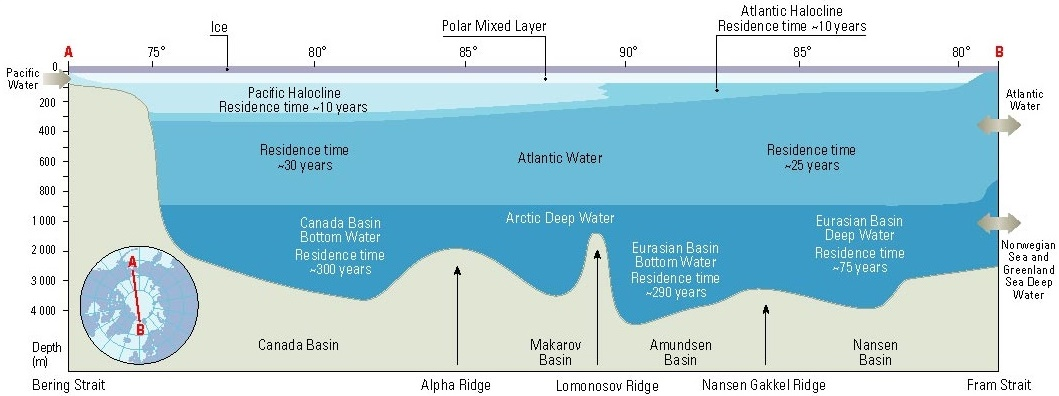
\includegraphics[width=\linewidth]{amap}
	\caption[\cite{wilson1998amap}]{  A schematic representation of the four-layer structure of the Arctic Ocean, with the Mixed Layer and Halocline
		above the Atlantic Water and Arctic Deep Water (\cite{aagaard1989role}). 
		The residence time for the different water masses are also shown (\cite{bonisch1995deep}). \cite{wilson1998amap}.}
	\label{fig:amap}
\end{figure}

Because of the strong stratification, the forcing from the ocean surface 
struggles to penetrate deep into the ocean; and so whether forced directly by wind 
or by sea ice stress, the circulation
directly forced from the surface is contained within the Polar Mixed Layer 
and halocline in the upper ${\sim}200\,\mathrm{m}$ of the Arctic Ocean. 
This surface circulation has been well documented by observations
from cruises and moorings  dropped  from  the  ice  shelf  or  deployed  on 
the  shallower  continental  shelves (\cite{gerdes1997large}, \cite{jones2001circulation}). On the other hand, it is a very different
story for the circulation in the \gls{awl} and lower layers. Observations made
inside the Ocean's basins rarely are able to profile the structure  and
circulation  below 500m  although much progress has been made here in the
past decade. This lack of observations means that  we  still only have  a  sense  of  the circulation 
of the \gls{awl} and the Deep  Waters.  The  observations  we  do 
have  infer stable cyclonic  rim  currents about each of the basins in the
\gls{awl} and it is believed that this trend extends through the Deep Water to the 
ocean floor (\figref{fig:Proshutinsky2005Circulation}).  It is apparent that the surface flows have little correlation with these deep circulations, this is because of the 
strong stratification in the halocline, and hence only leaves a handful of other possibilities for determining the processes that set the deep water circulation.


\begin{figure}
	\centering
	\includegraphics[width=0.9\linewidth]{Proshutinsky2005Circulation}
	\caption[\cite{proshutinsky2005arctic}]{ Two freshwater layer regimes (light 
		blue arrows) overlaying the cyclonic rim currents of the \gls{awl} (red arrows).
		Whilst the Freshwater regimes are vastly different from each other, the
		\gls{awl} is unaffected and remains persistently cyclonic.
		Topography is represented in the background running from 
		shallow water (light blue) to deep water (dark blue).  \cite{proshutinsky2005arctic}.}
	\label{fig:Proshutinsky2005Circulation}
\end{figure}

There has been much discussion
into how the fluxes in and out of the Arctic could influence the circulation,
for example, by a forcing a balance of \gls{pv} within the region by
the fluxes of \gls{pv} though the boundaries. \cite{yang2005arctic} demonstrates how,
in an idealised barotropic model of a basin, controlling the flux 
of \gls{pv} through inflows and outflows
at the boundary, the circulation in the basin could be switched between cyclonic and
anti-cyclonic circulations (\figref{fig:Yang2005}). This principle suggests
that the persistent cyclonic nature of the \gls{awl} is induced by a 
net influx of \gls{pv} via the Arctic Gateways. Fortunately, permanent moorings 
covering the majority of the ocean gateways into the Arctic~Ocean have built
up a detailed picture of the transport in and out of the Arctic Ocean 
(\cite{tsubouchi2012arctic}, \figref{fig:Tsubouchi2012Transport}). The net flux of \gls{pv} is then estimated by summing the distribution of \gls{pv}; given by $ \Pi_{i} = fQ_{i}/H_{i}$,
where $Q_{i}$ is the volume transport and $H_i$ the depth, for location $i$. 
Whilst there is a tendency for total to infer a positive influx of \gls{pv}, the
results are not convincing; \cite{munchow2006observational} shows that by including the
Canadian Archipelago in the \cite{yang2005arctic} calculation the flux can be negated whilst
\cite{tsubouchi2012arctic} demonstrates large variations of transport from the mean over time.
These factors, especially the large variability, make it unconvincing that its the \gls{pv}
 transport, or in fact any properties of the gateway fluxes, that determines the 
cyclonic nature of the \gls{awl}.
Hence, the deep water circulation in the Arctic Ocean is most likely determined by 
internal processes, which are poor understood, especially in an Ocean with such sparse observations.

\begin{figure}
	\centering
	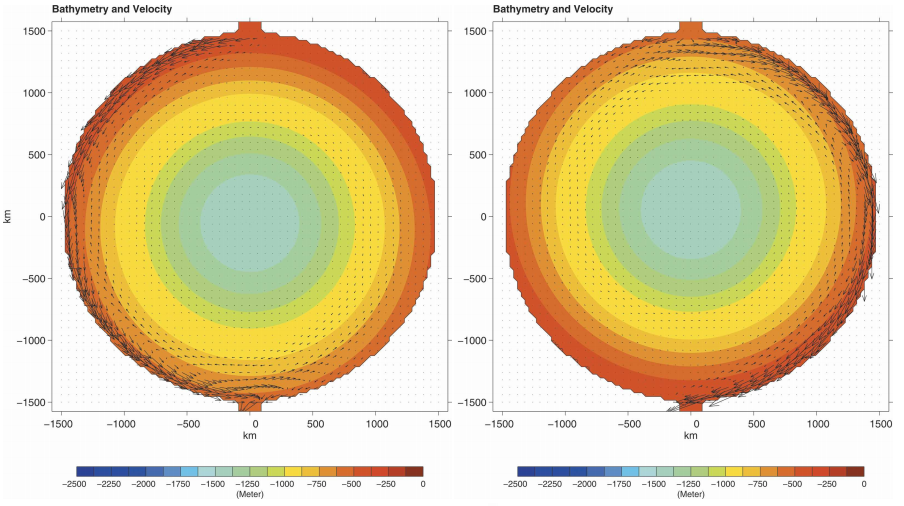
\includegraphics[width=\linewidth]{Yang2005}
	\caption[\cite{yang2005arctic}]{ The circulation of two simple barotropic
		models. The background colour is the model bathymetry. The left plot has
		a net influx of \gls{pv} (the inflow is shallower than the outflow) 
		and a cyclonic circulation whilst the right plot has net outflux of  \gls{pv} 
		and an anti-cyclonic circulation. \cite{yang2005arctic}.}
	\label{fig:Yang2005}
\end{figure}


\begin{figure}
	\centering
	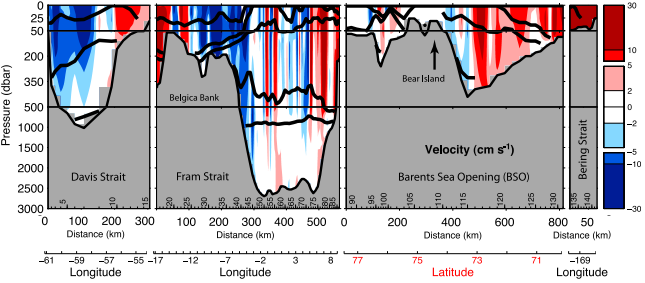
\includegraphics[width=\linewidth]{Tsubouchi2012Transport}
	\caption[Adapted from \cite{tsubouchi2012arctic}]{Velocity
		sections ($\mathrm{cm}\, \mathrm{s}^{-1}$) from Arctic gateway mooring arrays;
		Demonstrates the pathways through the gateways, from which transport 
		in to the Arctic can be calculated.
		Bold black lines show certain isopycnals, and the red (blue) colors show inflow
		into (outflow from) the Arctic.  Adapted from \cite{tsubouchi2012arctic}.}
	\label{fig:Tsubouchi2012Transport}
\end{figure}

A likely candidate for generating a cyclonic circulation in the Northern hemisphere is
geostrophic turbulence. A number of studies have demonstrated how, in an eddying system, 
sloping topography can generate along-topography flows (\cite{treguier1989topographically}, \cite{adcock2000interactions}, \cite{nost2008asymmetry}). Hence, in the absence of stronger
forcing, this effect is likely to become the dominant feature. An obvious question that then
comes to mind is how turbulent is the Arctic Ocean? Over recent years a large amount  of 
effort has been made to observe and catalogue eddies in the Arctic
(\cite{zhao2014characterizing}) and has demonstrated their prevalence in the Arctic Ocean.
Whilst these studies have frequently been focused on the halocline and the surface dynamics
there is good reason to believe that eddies also penetrate deep into the Arctic 
(\figref{fig:Woodgate2001Mooring}, \cite{woodgate2001arctic}).



\begin{figure}
	\centering
	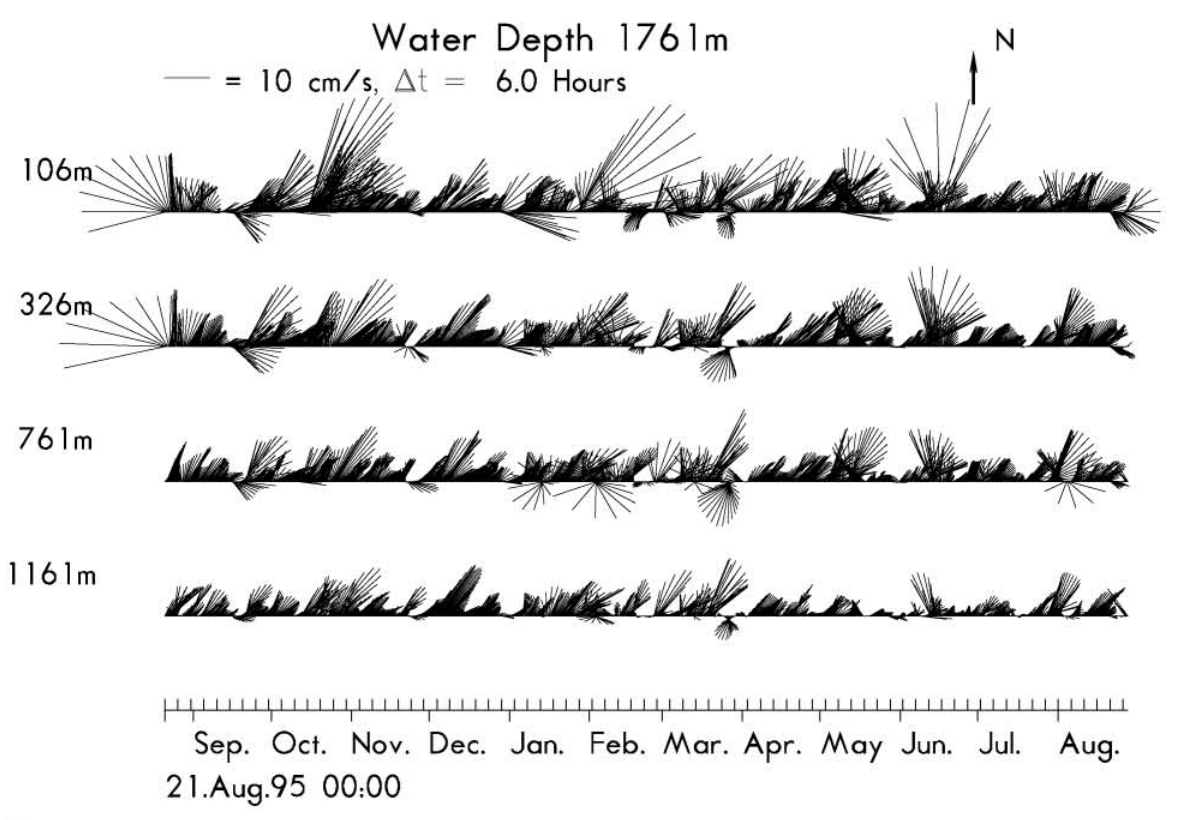
\includegraphics[width=\linewidth]{Woodgate2001Mooring}
	\caption[Adapted from \cite{woodgate2001arctic}]{A Velocity Stickplot 
		from a year-long mooring at \ang{78;30.8;} N, \ang{133;57.7;} E, west of the Lomonosov Ridge.  The plot shows a huge amount of variability over time, with many
		features being persistent throughout the water column. Adapted from \cite{woodgate2001arctic}.}
	\label{fig:Woodgate2001Mooring}
\end{figure}

\section{Mean-Eddy Interaction Theory}

\label{meaneddyinteractiontheory}

 Obviously, whilst observations play a vital role in understanding the Arctic
 Ocean and its role in the global ocean, it is limited by the sparsely available
 observations that only usefully reach back a handful of decades into the past.
 To be able to test possible scenarios and make future predictions it is vital
 that we have reliable simulations of the Arctic Ocean (\cite{proshutinsky2008toward});
 however, due to limitations
 in modern computing power and poor understanding of the unresolved processes 
 in the ocean this is, more often than not, far from reality.
 Due to these computational limits a practical \gls{gcm} is 
 limited to a  resolution of the order of tens of kilometres. This means that with a 
 resolution  cut off at around $10 \textendash 100 \, \mathrm{km}$, 
 \glspl{gcm} are unable to fully resolve a large portion of the mesoscale turbulence that is
 observed in the physical ocean.
 By attempting  to understand the physics behind these unresolved processes 
 and developing parameterisations that mimic their effect on the resolved ocean
 the value of computational models can be improved without dramatically increasing the
 computing power required.  
 
 The turbulent, chaotic nature of the ocean is caused by the non-linearity of its 
 governing equations. Because of this,  the discretisation of the equations generates cross-correlation, or eddy, terms when applying the 
 averaging operator,
 \begin{equation}
 \mean{\phi\psi} = \mean{\phi}\,\mean{\psi} + 
 \mean{\res{\psi}\res{\psi}},
 \label{non-lin average}
 \end{equation}
 where the ${\mean{\phi}}$ is the average of the variable ${\phi}$, used in
 the discretisation and satisfying
 the expected properties of an averaging operator, and the prime denotes the residual, ${\phi^{\prime} = \phi - \mean{\phi}}$.
 The discretised system has no knowledge of the residual terms and hence
 the contributions to the full system by these eddy terms are
 ignored in the discretised system. It is, therefore, this ``sub-grid scale process"
 that is missing from the model dynamics and so it is common practise to try and
 `close' the system by including a parameterisation of the eddy
 term in place of the term itself, which is usually dependent on the averaged 
 variables and some physical assumptions.
 
 \subsection{\cite{gent1990}}
 
 The earliest ocean models (\cite{bryan1969numerical}) had vertical $z$-coordinate, or depth-coordinates, with simple horizontal and vertical Laplacian diffusion to act as 
 the closure. Whether these terms are interpreted as a parameterisation for the effects
 of unresolved turbulence or simply as a numerical tool to avoid noise at 
 the grid scale, the viscosity parameter is tuned such that the turbulent energy cascade is 
 dissipated at the grid scale whilst still allowing as active dynamics as possible. 
 Assuming modern day computing power this implies a horizontal viscosity of around 
 $10^{5} - 10^{7} \mathrm{Pa} \cdot \mathrm{s}$, a viscosity more suited to peanut butter than 
 a the ocean. A second problem with having such a strong horizontal diffusion is
 that it diffuses or mixes tracers horizontally, when applied as
 an eddy parameterisation for tracer mixing. It has long been understood that tracers 
 mix much more along isopycnal surfaces than across them (\cite{iselin1939influence}, \cite{montgomery1940present}), which is a property which allowed for the definition of
 distinct water masses in the global ocean (for example, \cite{emery1986global}).
  Hence, with an excessive horizontal diffusion
 of tracers ocean models are able to break up water masses much quick than
 is observed in the physical ocean creating, for example, the ``Veronis Effect" (\cite{veronis1975role}).
 Hence, a more physically appropriate eddy parameterisation 
 is needed;
  and so, in a way that seems obvious today, eddies need to be
   parameterised in 
 such a way that their effect acts along isopycnal surfaces. 
 The effort to do this in the 80's and early 90's gave birth
 to what is known as the \gls{gm}, first introduced in \cite{gent1990}.
 
 So what is the \gls{gm} parameterisation? Since mixing occurs primarily
 along isopycnal surfaces it make sense to have this discussion in
 isopycnal coordinates, that is in the coordinate space $(x,y,\rho)$,
  where density, $\rho$, has replaced depth, $z$, as the vertical
  coordinate. Whilst the rigorous exploration of this coordinate system
  will be discussed in detail later on, in the \secref{youngtwa}, for our current purposes 
  it is enough to say that this coordinate system produces an equation
  for isopycnal ``thickness",
  \begin{equation}
  \label{cont}
  \frac{\partial z_{\rho}}{\partial t} + \boldsymbol{\nabla}\cdot\left(z_{\rho}\boldsymbol{u}\right) = 0,
  \end{equation}
  where $z_{\rho} = \frac{\partial z}{\partial \rho}$ is defined as the
   isopycnal thickness and $\boldsymbol{u}$ is the horizontal fluid
   velocity. Since it is non-linear, when this equation is discretised
   it produces an eddy covariance term as demonstrated by 
   \equref{non-lin average}; the averaged equation can be written as
     \begin{equation}
     \frac{\partial \mean{z_{\rho}}}{\partial t} + \boldsymbol{\nabla}\cdot\left(\mean{z_{\rho}} \, \mean{\boldsymbol{u}}\right) = - \boldsymbol{\nabla}\cdot\left(\mean{\res{z_{\rho}} \res{\boldsymbol{u}}}\right).
     \label{meancont}
     \end{equation}
   The eddies should therefore be parameterised by some representation
   of $\mean{\res{z_{\rho}} \res{\boldsymbol{u}}}$, say $\boldsymbol{F}$,
   so that the thickness equation becomes
     \begin{equation}
     \frac{\partial z_{\rho}}{\partial t} + \boldsymbol{\nabla}\cdot\left(z_{\rho}\boldsymbol{u}\right) + \boldsymbol{\nabla}\cdot\boldsymbol{F} = 0,
     \label{thicknessgeneralparam}
     \end{equation}
    where the bars have been dropped for convenience. It can also 
    be noted that by defining $\hat{\boldsymbol{u}} = \boldsymbol{F}/z_{\rho}$ the above equation can be interpreted as
    the isopycnal thickness
    being advected by the mean horizontal velocity, $\boldsymbol{u}$, 
    plus an eddy induced
    `bolus velocity', $\hat{\boldsymbol{u}}$. \cite{gent1990} then goes one
    step further and proposes that eddies act to homogenise each
    isopyncal layer via baroclinic instability, hence the 
    \gls{gm} parameterisation is given by $\boldsymbol{F} = - \left(\kappa
    \boldsymbol{\nabla} z \right)_{\rho}$, where $\kappa$ can both be
     spatially and temporally varying parameter. Combining this with  \equref{thicknessgeneralparam} we have
          \begin{equation}
          \frac{\partial z_{\rho}}{\partial t} + \boldsymbol{\nabla}\cdot\left(z_{\rho}\boldsymbol{u}\right) = \boldsymbol{\nabla}\cdot\left(\kappa
              \boldsymbol{\nabla} z \right)_{\rho} .
              \label{contgm}
          \end{equation}
    Similarly, for a tracer, say $\tau$, we can write an equation
    describing it's transport,
            \begin{equation}
              \frac{\partial \tau}{\partial t} + \boldsymbol{u}\cdot\boldsymbol{\nabla}\tau = \boldsymbol{\nabla}\tau\cdot
              \left(\kappa \boldsymbol{\nabla} z \right)_{\rho}/z_{\rho} .
            \end{equation}
            
    There are a few properties of this parameterisation that can be 
    noted to help describe its overall effect of its implementation in
    ocean models. Firstly, by writing $\boldsymbol{u}^{\star} = \boldsymbol{u} -
    \left(\kappa \boldsymbol{\nabla} z \right)_{\rho}/z_{\rho}$ we 
    simply have that $\frac{\partial z_{\rho}}{\partial t} + \boldsymbol{\nabla}\cdot\left(z_{\rho}\boldsymbol{u}^{\star}\right) = 0$ and $\frac{\partial \tau}{\partial t} + \boldsymbol{u}^{\star}\cdot\boldsymbol{\nabla}\tau = 0$ indicating
    that the tracer $\tau$ is effectively advected by a transport velocity, 
     $\boldsymbol{u}^{\star}$. Secondly, an important 
    question is how does \gls{gm} change the energy of the system. 
    The right hand side of \equref{contgm} adds 
    $\phi \boldsymbol{\nabla}\cdot\left(\kappa
                  \boldsymbol{\nabla} z \right)_{\rho} 
                  = \boldsymbol{\nabla}\cdot\left(\phi\kappa
                       \boldsymbol{\nabla} z \right)_{\rho} 
                  -\left(\kappa
              \boldsymbol{\nabla}\phi\cdot \boldsymbol{\nabla} z \right)_{\rho} 
                                -\left(\kappa g
                            \boldsymbol{\nabla}z\cdot \boldsymbol{\nabla} z \right)/{\rho_{0}} 
                $ to the energy tendency. Integrating over an entire domain
                eliminates the first two terms leaving the final term
                as a positive definite sink of energy. These two 
                properties characterise \gls{gm}; the parameterisation
                acts along isopycnal surfaces to flatten isopycnal 
                surfaces whilst dissipating potential energy.
                
        The dissipative nature of \gls{gm} is both an strength and a
         weakness. \gls{gm} is incapable of introducing spurious energy,
         which allows it to be very robust and stable meaning it can be implemented 
         into a \gls{gcm} with little tuning. However, it is also understood that
         ocean turbulence is not purely dissipative.
          \cite{adcock2000interactions} concisely demonstrated that
         in an idealised model, with no external forcing other
         than an initial eddy field, will develop a persistent along
         topography flow and the isopycnals will dome slightly above topography.
          \cite{nost2008asymmetry} showed that these
         flows develop asymmetrically, such that the flow is 
         predominantly cyclonic in
         a basin in the northern hemisphere. For this to occur 
         when the eddy field is unresolved there must be an 
         injection of energy into the system representing the 
         inverse cascade of energy from the eddy scales to the large scale.
         However, this is prohibited by the purely dissipative \gls{gm}
         and so a different parameterisation is required to mimic this
         effect.
         
         
         
         \subsection{\gls{pv} Closure}
         
         To proceed one might wonder what makes the continuity equation
         so special, in truth there is a number of non-linearities that
         crop up when examining the full state equations. Take, for example, the
         absolute vorticity, which can be written in the same form as the continuity equation, i.e.
           \begin{equation}
           \frac{\partial \omega}{\partial t} + \boldsymbol{\nabla}\cdot\left(\omega\boldsymbol{u}\right) = 0,
           \label{vort}
           \end{equation}
           where $\omega=f+\xi$ is the absolute vorticity and
           $\xi = \boldsymbol{k} \cdot\left( \boldsymbol{\nabla}\wedge \boldsymbol{u}\right)$ is the relative vorticity. 
           By applying an average operator to \equref{vort}, we have the same averaged equation as \equref{meancont} but for the mean absolute vorticity, $\mean{\omega}$,
                \begin{equation}
                \frac{\partial \mean{\omega}}{\partial t} + \boldsymbol{\nabla}\cdot\left(\mean{\omega} \, \mean{\boldsymbol{u}}\right) = - \boldsymbol{\nabla}\cdot\left(\mean{\res{\omega} \res{\boldsymbol{u}}}\right),
                \end{equation}
                which to close in a numerical model requires the
                right hand side, $- \boldsymbol{\nabla}\cdot\left(\mean{\res{\omega} \res{\boldsymbol{u}}}\right)$, to be parameterised.
                \cite{greatbatch1998exploring} makes the observation
                here that the mechanism this equation is describing 
                is much clearer if we note the following; if we take
                $\mean{q}$ to be the thickness weighted mean of $q$, i.e.
                $\mean{q}=\mean{z_{\rho}q}/\mean{z}_{\rho}$, then 
                $\mean{\omega}=\mean{q}\,\mean{z}_{\rho}$ and $\res{\omega}=\mean{z}_{\rho}\res{q}+\mean{q}\res{z}_{\rho}$. By 
                combining this with \equref{meancont} we gain a conservative equation 
                for \gls{pv}, 
                \begin{equation}
                \frac{\partial \left(\mean{z}_{\rho} \mean{q}\right)}{\partial t} +
                 \boldsymbol{\nabla}\cdot\left(\mean{z}_{\rho}\,\mean{q}\,\mean{\boldsymbol{u}}+\mean{q}\mean{\res{z}_{\rho} \res{\boldsymbol{u}}}\right)
                 = - \boldsymbol{\nabla}\cdot\left(\mean{z}_{\rho}\,\mean{\res{q} \res{\boldsymbol{u}}}\right) .
                 \label{meanpveq}
                \end{equation}
                This being the form of \gls{pv}, which leads to the impermeability theorems
                of \cite{haynes1987evolution} and \cite{haynes1990conservation}.
                
                Now, by making the same assumption that was made for isopycnal thickness in 
                \gls{gm} for \gls{pv}, that ocean eddies mix PV along isopycnals in the down-gradient direction, \equref{meanpveq} becomes
                \begin{equation}
                \frac{\partial \left(\mean{z}_{\rho} \mean{q}\right)}{\partial t} +
                \boldsymbol{\nabla}\cdot\left(\mean{z}_{\rho}\,\mean{q}\,\mean{\boldsymbol{u}}+\mean{q}\mean{\res{z}_{\rho} \res{\boldsymbol{u}}}\right)
                = \boldsymbol{\nabla}\cdot\left(\kappa \mean{z}_{\rho}\,\boldsymbol{\nabla}\mean{q}\right) ,
                \label{parammeanpveq}
                \end{equation}
                where the small slope approximation has been used, as demonstrated in
                \cite{gent1990}. By using Equations~\ref{meancont}~and~\ref{parammeanpveq} we have exactly the equation for an arbitrary tracer given in Equation 6 of \cite{gent1995parameterizing},
                \begin{equation}
                \frac{D^\star \mean{q}}{D t}\equiv\frac{\partial \mean{q}}{\partial t} + \boldsymbol{u}^\star\cdot\boldsymbol{\nabla}\mean{q} = \boldsymbol{\nabla}\cdot
                \left(\kappa \mean{z}_{\rho}\boldsymbol{\nabla} \mean{q} \right)/\mean{z}_{\rho} ,
                \label{pvclosure}
                \end{equation}
                applied to the mean \gls{pv}, which is advected by the transport velocity $\boldsymbol{u}^\star$ and diffused along isopycnal surfaces. This is now
                the \gls{pv} closure first proposed in \cite{greatbatch1998exploring}.
                
                \equref{pvclosure} represents the interaction of eddies as the
                down-gradient diffusion of \gls{pv}; and hence suggests that eddies
                act to homogenise \gls{pv}. Since \gls{pv} can be approximately written
                as $q=f/\sigma$ for small relative vorticity, the parametrisation acts  to homogenise isopycnal thickness. In the case 
                where there is no topography this is identical to the flattening of isopycnals.
                However, in the presence of topography homogenised isopycnal thickness
                causes the isopycnals to mimic the shape of the topography and hence 
                rise over topography. Unfortunately, to allow this to happen freely
                clearly violates energy conservation, as demonstrated schematically in 
                \figref{fig:Colddoming}. In reality, the ocean attempts to 
                homogenise \gls{pv} but only so far as it can with the available energy;
                the result is the slight ``cold doming" above topography as observed in
                \cite{adcock2000interactions}. 
                
                It isn't all bad news though. Whilst, unlike \gls{gm}, the downgradient
                dissipation of \gls{pv} capable of introducing spurious energy, it does
                control another important quantity: Enstrophy. By multiplying through 
                by $\mean{z}_{\rho} \mean{q}$, \equref{pvclosure} becomes 
                \begin{equation}
                \frac{\partial  }{\partial t}\left(\half z_{\rho}q^{2}\right) + \boldsymbol{\nabla}\cdot\left(z_{\rho}q\boldsymbol{u}^\star-\kappa z_{\rho}q\boldsymbol{\nabla} q
                \right)=-\kappa z_\rho \boldsymbol{\nabla}q\cdot\boldsymbol{\nabla}q
                \end{equation}
                where the bars have been dropped for convenience.
                Integrating over the entire domain eliminates the divergent term
                leaving just a positive definite dissipation.
                Hence, in the same way that \gls{gm} dissipates potential energy, this
                \gls{pv} closure dissipates enstrophy. This suggests the tantalising
                possibility that eddy-mean interactions are \gls{gm}-like when
                there is limited eddy energy available but diffuse \gls{pv} when
                limited by eddy enstrophy.
                
                \begin{figure}
                	\centering
                	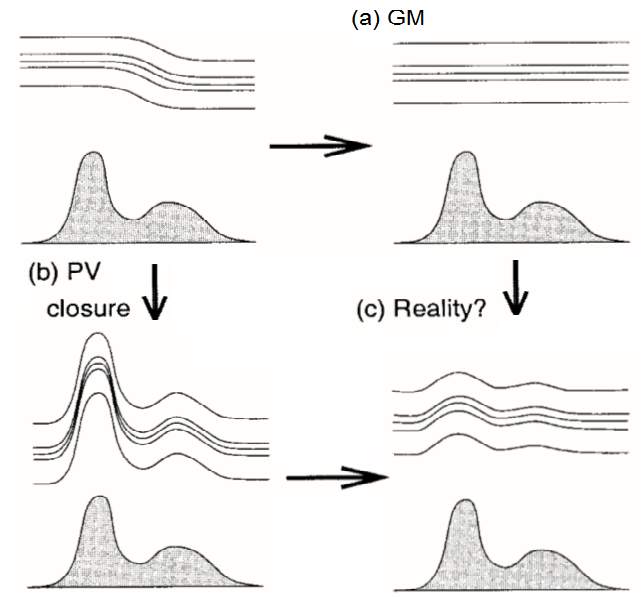
\includegraphics[width=0.6\linewidth]{am00}
                	\caption[Cold-doming]{\hl{I'm going to redraw these for the basin case.}}
                	\label{fig:Colddoming}
                \end{figure}
                
                
                
                \subsection{Eliassen-Palm Flux Tensor}
                
                It is clear from these attempts to parameterise the eddy-mean interaction
                that the only way to proceed is by being able to take into account 
                all eddy correlations that appear in the state equations. Residual-mean theory
                allows the directionally averaged primitive equations to be written such that 
                only diabatic buoyancy
                fluxes only appear in the thermodynamic equation whilst the eddy-mean
                interactions in the momentum equations appear as the divergence of Eliassen-Palm 
                Flux vectors (\cite{eliassen1961transfer}, \cite{andrews1976planetary}). 
                The Eliassen-Palm flux vectors also appear in other descriptions of ocean dynamics.
                In the averaged hydrostatic primitive equations the eddy-mean interactions
                appear as two Eliassen-Palm flux vectors, one for each component of the horizontal velocity
                (\cite{young2012exact}). Similarly, a rank-two Eliassen-Palm flux tensor
                can be derived for the statistically steady quasi-geostrophic equations (\cite{cronin1996eddy}). \cite{maddison2013eliassen} demonstrates
                the geometric relationship between Eliassen-Palm fluxes and how they
                collapse into a single coordinate invariant tensor in the
                quasi-geostrophic limit up to a gauge transformation.
                In this limit the Eliassen-Palm flux tensor can be written as
                \begin{equation}
                \boldsymbol{E} 
                =\left(  \begin{array}{ccc}
                -M+P &
                N & 0 \\
                N &  
                M + P & 0\\
                -S  &  
                R & 0\\
                \end{array} \right) 
                \end{equation}
                (\cite{plumb1986three}), where 
                \begin{equation}
                \begin{array}{ccc}
                M = \frac{\mean{{\res{v}}^{2} - {\res{u}}^{2}}}{2}, & 
                N = \mean{\res{u}\res{v} }, &
                P =  \frac{\mean{{\res{b}}^{2}}}{2\mathcal{N}_{0}^{2}},  \\ 
                R =  \frac{f_{0}}{\mathcal{N}_{0}^{2}}\mean{\res{b}\res{u}}, \, & \rm and  &  
                S = \frac{f_{0}}{\mathcal{N}_{0}^{2}}\mean{\res{b}\res{v}} ;
                \end{array} 
                \end{equation}
                 and where $f_{0}$ is the mean value of the Coriolis parameter and $\mathcal{N}_{0}$ is the buoyancy frequency. \cite{marshall2012framework}
                demonstrates that by taking a weighted Frobenius norm on $\boldsymbol{E} $
                and applying the Cauchy-Schwarz inequality a handful of times the 
                 tensor is bounded by the eddy energy ${\left\|\boldsymbol{E}\right\|\leq\left(K+P\right)\equiv E}$,
                 where $K=\frac{\mean{{\res{u}}^{2} + {\res{v}}^{2}}}{2}$ is the eddy
                 kinetic energy.
                 Without any loss of generality, this bound allows us to rewrite the components of the tensor in the form
                 \begin{equation}
                 \begin{array}{cc}
                 M = -\gamma_{m}E\cos{2\phi_{m}}\cos^{2}{\lambda}, & 
                 N = \gamma_{m}E\sin{2\phi_{m}}\cos^{2}{\lambda}, \\
                 P =  E\sin^{2}{\lambda}, &  K =  E\cos^{2}{\lambda},  \\
                 R =  \gamma_{b}\frac{f_{0}}{\mathcal{N}_{0}^{2}}E\cos{\phi_{b}}\sin{2\lambda}, &
                 S = \gamma_{b}\frac{f_{0}}{\mathcal{N}_{0}^{2}}E\sin{\phi_{b}}\sin{2\lambda} .
                 \end{array} 
                 \end{equation}
                 Here we have introduced two eddy anisotropies, $0\leq\gamma_{m},\gamma_{b}\leq1$, two eddy flux angles $0\leq\phi_{m},\phi_{b}\leq\pi$ and an eddy energy partition angle,
                 $0\leq\lambda\leq\pi/2$. Now the Eliassen-Palm flux tensor
                 is written in terms of five non-dimensional, bounded parameters
                 and $E$, the eddy energy.
                 
                 
                 
                 \subsection{Thickness Weighted Averaging}
                 \label{youngtwa}
                 
                Returning to the Arctic Ocean as discussed in \secref{arcticocean},
                the ocean is a relatively quiescent and highly stratified ocean. 
                With that in mind, an appropriate framework for describing
                the dynamics of the Arctic is the hydrostatic primitive equations
                in isopycnal coordinates. \cite{young2012exact} carefully constructs
                these equations from Cartesian coordinate hydrostatic primitive equations,
                \begin{subequations}
                	\begin{equation}
                	\frac{D u}{D t} -fv + p_{x} = \mathcal{X} \\
                	\end{equation}
                	\begin{equation}
                	\frac{D v}{D t} +fu + p_{y} = \mathcal{Y} \\
                	\end{equation}
                	\begin{equation}
                	p_{z} = b \\
                	\end{equation}
                	\begin{equation}
                	u_{x} + v_{y} + w_{z} = 0 \\
                	\end{equation}
                	\begin{equation}
                	\frac{D b}{D t} = \omega,
                	\end{equation}
                \end{subequations}
                where $b(\boldsymbol{x},t)$ is the buoyancy,
                 $\rho=\rho_{0}\left(1-g^{-1}b\right)$; $\mathcal{X}$, $\mathcal{Y}$
                 denote adiabatic processes and body forces and $\omega$ represents
                 any diabatic forcing. In isopycnal coordinates this becomes
                 \begin{subequations}
                 	\label{isopyceq}
                 	\begin{equation}
                 	\frac{D u}{D t} -fv + m_{x} = \mathcal{X} \\
                 	\end{equation}
                 	\begin{equation}
                 	\frac{D v}{D t} +fu + m_{y} = \mathcal{Y} \\
                 	\end{equation}
                 	\begin{equation}
                 	m_{b} + \eta = 0  \\
                 	\end{equation}
                 	\begin{equation} 
                 	\label{isopyccont}
                 	\frac{\partial \sigma}{\partial t}  + \left( \sigma u\right)_{x} + \left( \sigma v\right)_{y} + \left( \sigma \omega\right)_{b} = 0 .
                 	\end{equation}
                 \end{subequations}
                 Here $z \equiv \eta(x,y,b,t) $, where $\eta$ is used to distinguish 
                 it has a dependent function; $\frac{D}{Dt} \equiv \frac{\partial}{\partial t}
                 + u\frac{\partial}{\partial x} + v\frac{\partial}{\partial y}
                 + \omega\frac{\partial}{\partial b}$ is the
                  convective derivative in isopycnal coordinates; $m \equiv p-b\eta$ is the 
                  Montgomery potential and $\sigma \equiv \eta_{b} = -m_{bb}$.
                  Compare the continuity equation, \equref{isopyccont}, with 
                  \equref{cont}, noting that
                  $\sigma = \eta_{b}$ is equivalent to $-z_{\rho}$. Using Equations~\eqref{isopyceq}, an energy equation can also be derived,
                  \begin{equation}
                  \frac{\partial \sigma K}{\partial t} + \frac{\partial P}{\partial t} = -\boldsymbol{\nabla}\left(\sigma K \boldsymbol{u} +
                  \sigma m \boldsymbol{u}\right) -\left(\frac{\partial \eta}{\partial t} m\right)_{b}, \\
                  \label{isopycenergyeq}
                  \end{equation}
                  taking $\mathcal{X}$, $\mathcal{Y}$ and $\omega$ to be zero and where $K=\half \left| \boldsymbol{u}\right|^{2}$ is kinetic energy and
                  $P=\eta^{2}$ is potential energy, integrating over the entire domain
                  integrates the right hand side to zero. 
                  Now, by defining a thickness weighted average,
                  $\thkmean{\psi}=\nthkmean{\sigma\psi}/\nthkmean{\sigma}$, where
                  $\nthkmean{\psi}$ is the standard average and their residuals,
                  $\thkres{\psi}=\psi-\thkmean{\psi}$ and $\nthkres{\psi}=\psi-\nthkmean{\psi}$,
                  \cite{young2012exact} constructs the Eliassen-Palm flux vectors, 
                  $\boldsymbol{E}^{u}$ and $\boldsymbol{E}^{v}$,  for
                  these equations so that the momentum equations become
                  \begin{subequations}
                  	\label{thkweigheq}
                  	\begin{equation}
                  	\frac{\spec{D} \thkmean{u}}{D t} -f\thkmean{v} + \nthkmean{m}_{x} 
                  	+\nthkmean{\sigma}^{-1}\boldsymbol{\nabla}\cdot\boldsymbol{E}^u= \thkmean{\mathcal{X}} \\
                  	\end{equation}
                  	\begin{equation}
                  	\frac{\spec{D} \thkmean{v}}{D t} +f\thkmean{u} + \nthkmean{m}_{y}
                  	+\nthkmean{\sigma}^{-1}\boldsymbol{\nabla}\cdot\boldsymbol{E}^v = \thkmean{\mathcal{Y}}, \\
                  	\end{equation}
                  	where $\frac{\spec{D} }{D t} = \equiv \frac{\partial}{\partial t}
                  	+ \thkmean{u}\frac{\partial}{\partial x} + \thkmean{v}\frac{\partial}{\partial y}
                  	+ \thkmean{\omega}\frac{\partial}{\partial b}$ is the
                  	mean convective derivative, whilst the continuity equation is just
                  	\begin{equation} 
                  	\frac{\partial \nthkmean{\sigma}}{\partial t}  + \left( \nthkmean{\sigma} \thkmean{u}\right)_{x} + \left( \nthkmean{\sigma} \thkmean{v}\right)_{y} + \left( \nthkmean{\sigma} \thkmean{\omega}\right)_{b} = 0 .
                  	\end{equation}
                   $\boldsymbol{E}^{u}$ and $\boldsymbol{E}^{v}$ are defined as
                   \begin{equation}
                   \label{youngtwaeptensor}
                   \begin{array}{c}
                   \boldsymbol{E}^{u}=\nthkmean{\sigma}\left(
                   \begin{array}{c}
                   \thkmean{\thkres{u}\thkres{u}} \\
                   \thkmean{\thkres{u}\thkres{v}} \\
                    \thkmean{\thkres{u}\thkres{\omega}} \\
                   \end{array}\right)+\left(
                   \begin{array}{c}
                   \half \nthkmean{\nthkres{\eta}\nthkres{\eta}} \\
                   0 \\
                   \nthkmean{\nthkres{\eta}\nthkres{m}_{x}} \\
                   \end{array}\right), \\ \\
                   \boldsymbol{E}^{v}=\nthkmean{\sigma}\left(
                   \begin{array}{c}
                   \thkmean{\thkres{u}\thkres{v}} \\
                   \thkmean{\thkres{v}\thkres{v}} \\
                   \thkmean{\thkres{v}\thkres{\omega}} \\
                   \end{array}\right)+\left(
                   \begin{array}{c}
                   0\\
                   \half \nthkmean{\nthkres{\eta}\nthkres{\eta}} \\
                   \nthkmean{\nthkres{\eta}\nthkres{m}_{y}} \\
                   \end{array}\right). \\
                   \end{array}
                   \end{equation}
                \end{subequations}
                   Crucially, in \cite{young2012exact} the first two components of  $\boldsymbol{E}^{u}$ and $\boldsymbol{E}^{v}$ are directed along 
                   the isopycnals, whilst only  the third component directed through 
                   isopycnal surfaces; hence, in the adiabatic case (i.e. when $\omega=0$)
                   $ \nthkmean{\sigma}^{-1}\nthkmean{\nthkres{\eta}\nthkres{m}_{x}}$ and 
                   $\nthkmean{\sigma}^{-1}\nthkmean{\nthkres{\eta}\nthkres{m}_{y}}$ are
                   precisely the ``inviscid pressure drag"  or ``form drag" identified
                   by \cite{rhines1979theoretical} and represents the transfer of momentum
                   between isopycnal surfaces. One key feature of this formulation
                   is that the eddy stresses are all entirely described in the momentum
                   equations, hence one might wonder what has happened to 
                   the bolus velocity described by \cite{gent1995parameterizing}. 
                   It turns out that the thickness weighted velocity is precisely 
                   the transport velocity, since $\thkmean{\boldsymbol{u}}=\nthkmean{\sigma\boldsymbol{u}}/\nthkmean{\sigma}=\nthkmean{\boldsymbol{u}} + \nthkmean{\nthkres{\sigma}\nthkres{\boldsymbol{u}}}/\nthkmean{\sigma}$
                   and  $\nthkmean{\nthkres{\sigma}\nthkres{\boldsymbol{u}}}/\nthkmean{\sigma}$
                   is the bolus velocity. Hence, this implies that  the equations explicitly
                    represent the mean velocities as the  transport velocities.
                     To retrieve the bounds derived by \cite{marshall2012framework} 
                     we write $\boldsymbol{E} = (\boldsymbol{E}^{u}, \boldsymbol{E}^{v}, 0)$
                     and note that in the geostrophic limit $m_x \sim fv$ and  $m_y \sim -fu$.
                     Then by writing 
                     \begin{equation}
                     \begin{array}{ccc}
                     M = \frac{\thkmean{{\thkres{v}}^{2} - {\thkres{u}}^{2}}}{2}, & 
                     N = \thkmean{\thkres{u}\thkres{v} }, \\
                     K = \frac{\thkmean{{\thkres{u}}^{2} + {\thkres{v}}^{2}}}{2}, & 
                     P =  {\nthkmean{{\nthkres{\eta}}^{2}}}/{\nthkmean{\sigma}},  \\ 
                     R =  f{\nthkmean{\nthkres{\eta}\nthkres{u}}}/{\nthkmean{\sigma}}, \, & \rm and  &  
                     S = f{\nthkmean{\nthkres{b}\nthkres{v}}}/{\nthkmean{\sigma}} ;
                     \end{array} 
                     \end{equation}
                     we have (in the adiabatic case) that
                     \begin{equation}
                     \boldsymbol{E}=\nthkmean{\sigma}\left(
                     \begin{array}{ccc}
                     -M+K+P & N & 0 \\
                     N & M+K+P & 0 \\
                     S & -R & 0 \\
                     \end{array}\right).
                     \end{equation}
                     By applying the Frobenius norm in a similar fashion to 
                     \cite{marshall2012framework} we retain the energy bound on
                      $\boldsymbol{E}$
                      
                      Equations~\equref{thkweigheq} are of the same form as Equations~\ref{isopyceq}.
                      Hence, it's possible to derive an
                      Rossby-Ertel \gls{pv} for the thickness weighted system
                      as
                      \begin{equation}
                      \frac{\spec{D} \spec{q}}{D t} + \nthkmean{m}_{x} 
                      +\nthkmean{\sigma}^{-1}\boldsymbol{\nabla}\cdot\spec{\boldsymbol{F}}
                      +\nthkmean{\sigma}^{-1}\boldsymbol{\nabla}\cdot\spec{\boldsymbol{\Gamma}}=0,
                      \end{equation} 
                      where
                      \begin{equation}
                      \spec{q}\equiv\frac{f+\thkmean{v}_{x}-\thkmean{u}_{y}}{\nthkmean{\sigma}},
                      \end{equation}
                      is the Rossby-Ertel \gls{pv}, $\Gamma$ contains only the diabatic terms involving $\thkmean{\mathcal{X}} $, $\thkmean{\mathcal{Y}} $ and $\thkmean{\omega} $ and 
                      \begin{equation}
                      \spec{\boldsymbol{F}}=\nthkmean{\sigma}^{-1}\left(
                      \begin{array}{c}
                      \boldsymbol{\nabla}\cdot\boldsymbol{E}^v \\
                      -\boldsymbol{\nabla}\cdot\boldsymbol{E}^u\\
                      0 \\
                      \end{array}\right).
                      \end{equation}
                      Hence, the \gls{pv} fluxes can be written in terms of
                      the momentum fluxes, whilst the momentum fluxes, ${\boldsymbol{\nabla}\cdot\boldsymbol{E}^u = -\nthkmean{\sigma} \spec{\boldsymbol{F}}\cdot\boldsymbol{j}}$ and                      ${\boldsymbol{\nabla}\cdot\boldsymbol{E}^v = \nthkmean{\sigma} \spec{\boldsymbol{F}}\cdot\boldsymbol{i}}$,
                      can be written in terms of the \gls{pv} fluxes.
                      Rather than $\spec{q}$, \cite{greatbatch1998exploring} suggest
                      the use of a thickness weighted Rossby-Ertel \gls{pv},
                      \begin{equation}
                      \thkmean{q}=\frac{\nthkmean{\sigma q}}{\nthkmean{\sigma}}=\frac{f+\nthkmean{v}_{x}-\nthkmean{u}_{y}}{\nthkmean{\sigma}},
                      \end{equation}
                      which leads  to
                      \begin{equation}
                      \frac{\spec{D} \left( \thkmean{q}\right)}{D t}
                      + \nthkmean{\sigma}^{-1}\boldsymbol{\nabla}\cdot\left(\nthkmean{\sigma}\thkmean{\thkres{q} \thkres{\boldsymbol{u}}}\right)
                      +\nthkmean{\sigma}^{-1}\boldsymbol{\nabla}\cdot\boldsymbol{\Upsilon}=0 ,
                      \end{equation}
                      where, again, $\boldsymbol{\Upsilon}$ only contains
                      diabatic terms. Compare with \equref{meanpveq}, and by noting that
                       ${\nthkmean{\sigma}\thkmean{\boldsymbol{u}}=\nthkmean{\sigma}\nthkmean{\boldsymbol{u}} + \nthkmean{\nthkres{\sigma}\nthkres{\boldsymbol{u}}}}$, we have the 
                       \cite{greatbatch1998exploring} form of \gls{pv} closure.
                       Using the Cauchy-Schwarz inequality, it is easily noted that
                       the norm of $\thkmean{\thkres{q} \thkres{\boldsymbol{u}}}$ is bounded
                       by $2\sqrt{KQ}$, where $K = \frac{\thkmean{{\thkres{u}}^{2} +
                       	{\thkres{v}}^{2}}}{2}$ is the eddy kinetic energy and $Q =
                        \frac{\thkmean{{\thkres{q}}^{2}}}{2}$ is the eddy enstrophy.
                       Providing $\spec{q} \sim \thkmean{q}$, which is equivalent 
                       to the  curl of the bolus velocities $\left(\nthkmean{\nthkres{\sigma}\nthkres{v}}/\nthkmean{\sigma}\right)_{x}-\left(\nthkmean{\nthkres{\sigma}\nthkres{u}}/\nthkmean{\sigma}\right)_{y}$ 
                       being small, then it can be assumed, in the adiabatic case,
                       that $\boldsymbol{\nabla}\cdot\spec{\boldsymbol{F}} \sim \boldsymbol{\nabla}\cdot\left(\thkmean{\thkres{q} \thkres{\boldsymbol{u}}}\right)$ and so $\spec{\boldsymbol{F}}$,
                       and hence $\boldsymbol{\nabla}\cdot\boldsymbol{E}$
                       is also bounded by  $2\sqrt{KQ}$.
                       
                       
                      
                      
                      
                      
                      
                      \subsection{Entropy  Maximisation}
                      \label{entropy}
                     
                
                \begin{itemize}    
                	
                	\item \hl{Entropy  Maximisation}
                	\begin{itemize}      
                		\item \hl{Rather than trying to discover a dynamical description of eddy stresses, an idea that eddies try to maximise entropy has been developing
                		in parallel.}
                		\item \cite{holloway1987systematic} \hl{demonstrated the principle with the idea that eddies in the ocean are like the jiggling of a box of marbles that randomises them into their highest state of entropy.}
                		\item \hl{This therefore becomes the problem of deriving the maximum
                		entropy state of the Ocean}
                		\begin{itemize}      
                			\item \cite{holloway1992representing} \hl{does this for a
                			 quasi-geostrophic ocean and by making a number of assumptions  
                			 arrives at a maximum entropy state which describes along 
                			 topography flow. Coined ``the Neptune Effect"}
                			\item \hl{other stuff}
                			\item \hl{Maximum Entropy Production. See} \cite{polyakov2001eddy}.
                		\end{itemize}
                		\item \hl{These principles inevitably give a solution for the ocean in 
                		a state of maximum entropy and then attempt to ``nudge" the ocean
                		towards the desired state. }
                		\item \hl{This could be reason if the ocean was subjected to unbounded 
                		energy, or ``jiggling", but in reality it is likely the ocean is never
                		pushed in the direction of maximum entropy production do to
                		a limitation of available energy.}
                	\end{itemize}  
                	
                \end{itemize}


\section{Numerical Models of Arctic}

	It was discussed in \secref{arcticocean} that to understand the circulation of the Arctic
	 Ocean it is necessary to use \glspl{gcm}. However, due to poorly resolved processes or
	  missing key physics, the \glspl{gcm} available show significant variability between
	   models and frequently display behaviour not depicted in observations. 
	A detailed comparison of the major Global Climate Models applied to the Arctic Ocean is
	 being carried out by the \gls{aomip} (see \cite{proshutinsky2008toward} and
	  \cite{proshutinsky2011recent}). In this section we will specifically discuss the skill
	   of these models in reflecting the Arctic circulation and specifically the difficulty
	    these models have in replicating the perceived flow in the Atlantic Water Layer.  

As mentioned in the previous section, the circulation in the freshwater layer is strongly
 governed by effects of surface forcing. To this extent, providing the various models being
  compared are given the same forcing, or equivalent depending on how the model is
   structured, then the resulting circulations are in good agreement
    (\cite{proshutinsky2005arctic}). They have been shown to have a good skill in imitating
     certain regimes which have been observed. However, despite good agreement of the general
      circulation inside the basin there is still some variation between the climate models.
       The first is how the Pacific Water entering via Bering Strait is advected through the
    basin within the freshwater layer. The models, despite showing the same regime for the
     Freshwater layer demonstrate different distributions of the Pacific Water when
      represented as a passive tracer added in Bering Strait (\cite{proshutinsky2011recent}).
       However, without an easy way of determining what water originates from the Pacific
        there are few observations available to determine the legitimacy of the models. The
     most successful attempts at determining the distribution of Pacific Water have been
     done using tracers from other sources, such as radioactive tracers from the Atlantic and
      determining where they?re being blocked by Pacific water such as in \cite{karcher2004dispersion}. More crucially models struggle to coherently and accurately represent
    mechanisms for the release of freshwater from the Arctic Ocean. This is most likely
     due to poor representation of the Arctic Gateways specifically in the Canadian
      Archipelago, where many of the straits and channels are much narrower than can be
   comfortably resolved. However, whilst these discrepancies are important, they are
    not the main focus here due to the overall competence of climate models to
 represent the freshwater layer in the Arctic. The more distressing problem is
  their ability to represent the Atlantic Water Layer. 

Observations suggest that the Atlantic Water Layer circulates counter clockwise around the
 Arctic basins at a depth of $200$ to $800\mathrm{m}$
 (\figref{fig:Proshutinsky2005Circulation}). However, many attempts over the past twenty
 years to model the Atlantic Water Layer have resulted in confusing predictions where the
 circulation seemingly randomly organises into circulations that are cyclonic or
 anti-cyclonic with almost identical frequency. To attempt to diagnose the skill of a model
 to produce cyclonic boundary currents \cite{holloway2007water} introduces ``topostrophy",
 defined as   $\tau=(\boldsymbol{f}\times\boldsymbol{V})\cdot\boldsymbol{\nabla}D$, where
 $\boldsymbol{f}$  is the Coriolis force,  $\boldsymbol{V}$ is velocity and  $D$ is the total
 depth. This so called topostrophy is a measure the strength of along slope flows and gives
 positive values for currents that flow with the upslope to their right (e.g. for cyclonic
 rim currents) and negative values for the opposite.  When calculated for the major
 \gls{aomip} models, most show variable and ambiguous values for $\tau$  whereas models that
 employ the ``Neptune Effect", mentioned in \secref{entropy}, shows a persistent and positive
 value for  $\tau$ (\cite{proshutinsky2011recent}). \cite{holloway2009representing} examine
 simultaneous simulations using the NEMO model run with and without the Neptune Effect and
 show that the addition of this particular parameterisation is the likely cause of this
 tendency (\figref{fig:HolloWang2009}).  


\begin{figure}
	\centering
	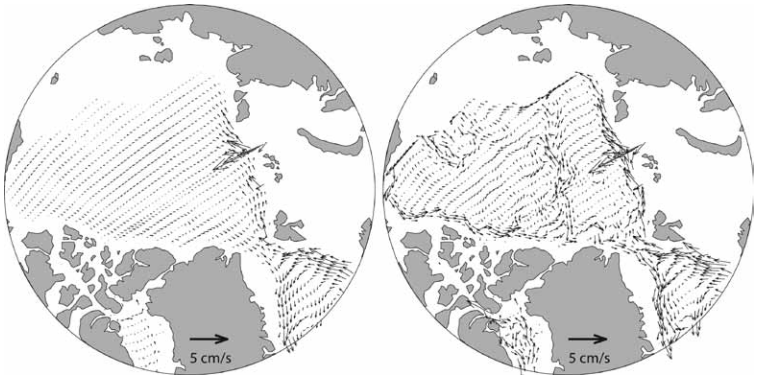
\includegraphics[width=\linewidth]{HolloWang2009}
	\caption[\cite{holloway2009representing}]{Left: The velocity field of the Arctic Ocean at 551m depth as simulated by the Nucleus for European Modeling of the Ocean (NEMO). Right: The velocity field at the same depth after NEMO was modified to include the Neptune Effect. The right panel clearly gives a better representation of the topographically aligned currents observed in the Arctic Ocean.  \cite{holloway2009representing}}
	\label{fig:HolloWang2009}
\end{figure}


\Gls{aomip} has demonstrated that \glspl{gcm} are woefully inadequate for predicting the
accurate circulation \gls{awl}. The evidence seems to suggest that this is because on 
climate time-scales a \gls{gcm} can at best be eddy-permitting and hence
lack the geostrophic turbulence that appears to be critical for setting the 
cyclonic circulation in the \gls{awl}. As discussed in \secref{meaneddyinteractiontheory},
the eddy parameterisations used in modern \glspl{gcm}, namely \gls{gm}, are too 
dissipative and fail to express the driving nature of eddy-topography interactions. 
The models that are more successful either better resolve the eddy fields or apply 
a corrective force, such as the ``Neptune Effect", in irresponsible manner. 

\section{Summary and Hypothesis}

Since the likes of \cite{young1982shear}, \cite{holloway1987systematic} and
\cite{gent1990}, we have seen much development of how to describe the mean-eddy interaction.
Attempting to parameterise this in non-eddy-resolving models has lead to 
continuity and \gls{pv} closure parameterisations such as \cite{gent1990}
and \cite{greatbatch1998exploring} as well maximum entropy principle parameterisations 
such as the ``Neptune Effect" (\cite{holloway1992representing}) and \cite{polyakov2001eddy}.
However, to date these parameterisations are hopeless over topography. Either
they are far to dissipative, like \gls{gm}, and fail to represent the driving nature
of eddies-topographic interactions or they violate energy conservation
by failing to appropriately control the energy injected into the system, as in the cases
of \gls{pv} closure and the ``Neptune Effect". To avoid this models attempting to
use non-dissipative parameterisations often attempt to tune the parameterisation in
an ad-hoc fashion to avoid spurious energy injection. However, by carefully implementing
the framework put forward by \cite{marshall2012framework} and generalised in
\cite{maddison2013eliassen}, one might create a parameterisation which is
inherently bounded by energy and enstrophy constraints.

The discussion in this Section has shown that the mean-eddy interactions 
emerge with competing \gls{gm}-like and ``Neptune Effect''-like natures
\cite{adcock2000interactions}. Meanwhile  it's possible to show that
the Eliassen-Palm flux tensor can be bounded by eddy energy and eddy enstrophy
\cite{marshall2012framework}.
Diagnosis of the contributions to the eddy stress tensor from
the eddy kinetic and potential energy, as well as the Reynolds' stress angle and eddy bouyancy flux angle will allow the investigation of the following:
\begin{itemize} 
		\item How much topographic slope is the controlling factor for the structure of the eddy stresses in eddy-topographic interactions.
		\item How limited energy is likely to inhibit the ability for the eddies the
			generate a mean along-topography flow.
	    \item That $\spec{q} \sim \thkmean{q}$ so that the enstrophy bound hold for $\spec{F}$,
		\item and hence, whether eddy stresses are limited by the available eddy enstrophy in the system.
\end{itemize} 
 

\chapter{Developement of Stacked Shallow Water Equations}
\label{sweq}

With the hope of taking advantage of the invariance demonstrated by 
\cite{maddison2013eliassen}, we need to be able to diagnose the
eddy terms in a controlled and repeatable environment. Hence, we turn our attention to
idealised models as a representation of ocean dynamics. This has an advantage 
over using observational data as well as output from \glspl{gcm} for a number of reasons.
\begin{itemize}
	\item The main limitation is that for this analysis to work, it must be possible to define an
	averaging operator that splits the eddy components of the system from the mean
	components, the most effective way of achieving this is to have a large data sample
	whose average is the mean state. Due to the lack of observational data, especially in the
	Arctic Ocean means that this  technique wouldn't be able to achieve an accurate or complete
	picture. 
	\item Similarly, defining what is meant by the ``mean component" is non-trivial in the physical ocean. Ideally, we would require a mean such that the residual term is precisely the 
	geostrophic turbulence that we are interested in. However, the ocean exhibits a multitude 
	oscillations and variability, such as seasonal and diurnal cycles, tides and many other
	non-linear effects from a combination of these and other processes, hence an average which
	is applied across this variability will include these effects in the residual components.
	\item This problem also applies to \glspl{gcm} which are often the culmination of 
	a number of generations of research and development with respect to ocean processes.
	This means that a \gls{gcm} often has numerous parameterisations and modules, which are
	designed to give a better representation of the ocean but make separating the useful components
	for this study non-trivial. 
	\item Finally, the complex nature of \glspl{gcm} mean that there is potentially a large saving
	of computational power than can be made by simplifying the problem into an idealised situation.
\end{itemize}

Starting from the full primitive equations we need to carefully make assumptions and
simplifications to create a representation of the ocean which is simple enough for our
purposes but still a close enough approximation to the ocean that any results are ultimately
 useful. Hence, we now set out the criteria required for such a model.
 \begin{itemize}
 	\item Firstly, the governing equations obviously must be non-linear or else there will be
 	no turbulence and nothing to diagnose.
 	\item The models must be able to cope with a realistic range of topographic slopes.
 	In the Arctic Ocean the sea floor drops by around $3000$ metres over $10$'s of kilometres
 	in places.
 	\item Baroclinic effects must be represented. It is well understood that a major role
 	of eddies is the baroclinic effect that \gls{gm} attempts to represent.
 	\item The model must be fast. The whole point of making these idealisation is to have model
 	 that can be run at high resolution quickly.
 	 \item As mentioned above, we must be able to define an averaging operator which 
 	 allows for the decomposition into a reasonable ``mean component" and ``eddy component".
 \end{itemize}
In this section we follow the development of such a model 


\section{Stacked Shallow Water Theory}
\label{swtheory}

For our study the equations that will give us the most efficient model whilst capturing the
 processes we would like are the stacked shallow water equations. Whilst this is a common
  simplification it is worth investigating whether it is an appropriate simplification to make
   here. 
   In deriving the shallow water equations we make approximations which are frequently made in
   most GFD analyses. The first of these approximations to make that is made is that the ocean
   incompressible or specifically the Boussinesq approximation. This is reasonable
   given the small size of deviations in density from the mean state
   that occurs in the ocean (\cite{vallis2006atmospheric}).
   The second approximation that is made is that the fluid is hydrostatic. That is to say that the equation $\frac{\partial p}{\partial z} + \rho g=0$ holds, where $p$ is pressure, $\rho$
   is density, $g$ is gravitational acceleration and $z$ is the vertical coordinate. Despite
   the fact that non-hydrostatic effects are likely to affect the vertical velocity, since
   there are only limited areas in the Arctic where dense water could overspill into less
   dense water, it is sensible to assume the hydrostatic approximation by scale arguments:
   the vertical components of velocity will be orders of magnitude smaller than the
   horizontal velocities. This give us the hydrostatic, Boussinesq  primitive equations:
   \begin{subequations}
   \begin{equation}
   \frac{Du}{Dt}-fv = -\frac{1}{\rho}   \frac{\partial p}{\partial x}+F_{u}-D_{u}, \\
   \end{equation}
   \begin{equation}
   \frac{Dv}{Dt}+fu = -\frac{1}{\rho}   \frac{\partial p}{\partial y}+F_{v}-D_{v}, \\
   \end{equation}
   \begin{equation}
   \frac{\partial p}{\partial z} + \rho g=0 \\
   \end{equation}
   \begin{equation}
   \frac{\partial u}{\partial x} + \frac{\partial v}{\partial y} +\frac{\partial w}{\partial z}  = 0 ,
   \end{equation}
   \end{subequations}
   where $(u,v)$ are the horizontal velocities, $w$ the vertical velocity, $f$ is the Coriolis
    parameter, and $F_{u}$, $F_{v}$, $D_{u}$ and  $D_{v}$ are the $u$- and $v$-components of
    the Forcing and  Dissipation.
    
    
    \begin{figure}
    	\centering
    	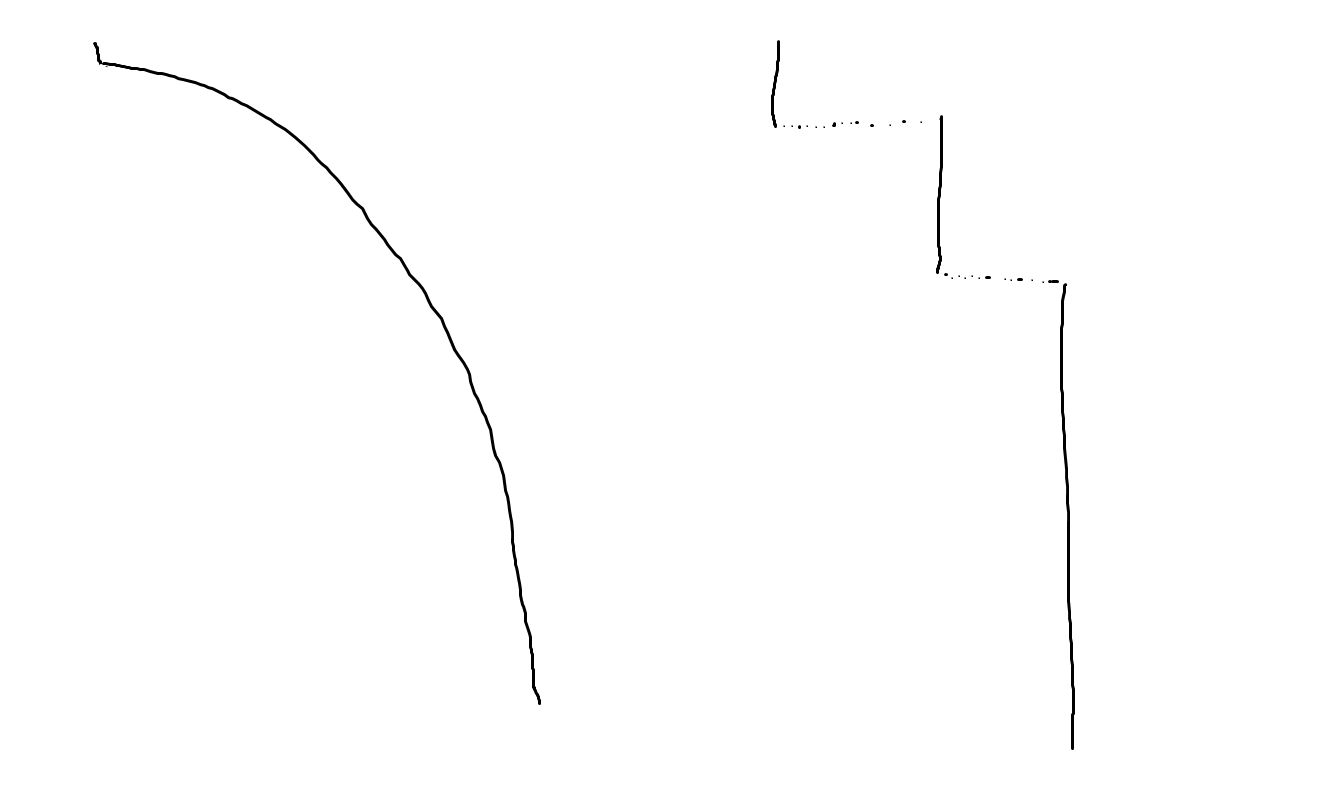
\includegraphics[width=0.5\linewidth]{SWDensity}
    	\caption[Shallow Water Density Profile]{  A more realistic  continuous
    		density profile (left) compared to the discontinuous, piecewise constant 
    		density profile of the stacked shallow water equations with 3 layers (right)}
    	\label{fig:swdensity}
    \end{figure}
    
    The next step is to approximate the vertical density profile as a stack of
    fluids of constant density, as in \figref{fig:swdensity}. 
    This is to allow the shallow
    water approximation to be made whilst allowing for baroclinic effects by 
    deriving the shallow water equations for each layer separately. Formally, 
    the density profile is split into $N$ sections with constant densities 
    $\rho_{1}$ through to $\rho_{N}$, where $n=1$ is the lowest layer and $n=N$
    is the uppermost layer. Integrating the hydrostatic equation, $\frac{\partial p}{\partial z} + \rho g=0$,
    downwards from the surface yields 
    \begin{equation}
    p(x,y,z)=\sum^{N}_{k=n+1}\left(g \rho_{k} h_{k} \right) + g \rho_{n}\left(\eta_{n+\half } - z \right)
    \end{equation}
    for $\eta_{n-\half }\leq z \leq \eta_{n+\half }$, where $\eta_{n+\half }(x,y,t)$,
    $\eta_{n-\half }(x,y,t)$ are the depths of the interfaces above and below layer $n$
    respectively and $h_{n} = \eta_{n+\half } -\eta_{n-\half }$ is the vertical
     thickness  of layer $n$. Similarly, by integrating the continuity equation over a layer
     we have
     \begin{equation}
     \begin{split}
     0 &=\int^{\eta_{n+\half }}_{\eta_{n-\half }}\left(\frac{\partial u}{\partial x} + \frac{\partial v}{\partial y} +\frac{\partial w}{\partial z} \right){\rm d} z \\
     &=\frac{\partial }{\partial x}\int^{\eta_{n+\half }}_{\eta_{n-\half }} u{\rm d} z +
     \frac{\partial }{\partial y}\int^{\eta_{n+\half }}_{\eta_{n-\half }} v{\rm d} z
      -  \left[ u   \frac{\partial z}{\partial x} \right]^{\eta_{n+\half }}_{\eta_{n-\half }} 
      -  \left[ v  \frac{\partial z}{\partial y}\right]^{\eta_{n+\half }}_{\eta_{n-\half }}  +
      \left[ w \right]^{\eta_{n+\half }}_{\eta_{n-\half }} \\
     &=\frac{\partial h_{n} }{\partial t} +\frac{\partial h_{n} u_{n}}{\partial x}+
     \frac{\partial h_{n} v_{n} }{\partial y},      \\
     \end{split}
     \end{equation}
   using that $w =  \frac{\partial z }{\partial t} + u \frac{\partial z}{\partial x} 
   + v \frac{\partial z}{\partial y}$ at $z = \eta_{n+\half } , \eta_{n-\half }$; $u_{n} =\frac{1}{h_{n}}\int^{\eta_{n+\half }}_{\eta_{n-\half }} u{\rm d} z$ and $v_{n} =\frac{1}{h_{n}}\int^{\eta_{n+\half }}_{\eta_{n-\half }} v{\rm d} z$. By also defining 
   the Montgomery potential as
   $m_{n}(x,y,t)=p+g \rho_{n} z=\sum^{N}_{k=n}\left(\rho_{N} g_{k+\half } \eta_{k+\half } \right) $ where 
   $g_{n+\half } =  \frac{\rho_{n} - \rho_{n+1}}{\rho_{N}}$, we have the stacked shallow water
   equations as derived in \cite{vallis2006atmospheric} and \cite{cushman2011introduction}, 
   \begin{subequations}
   	\label{sweqs}
   \begin{equation}
   \label{swumomeq}
   \frac{Du_{n}}{Dt}-fv_{n} = -\frac{1}{\rho_{n}}   \frac{\partial m_{n}}{\partial x}+F_{u_{n}}-D_{u_{n}}, \\
   \end{equation}
   \begin{equation}
   \label{swvmomeq}
   \frac{Dv_{n}}{Dt}+fu_{n} = -\frac{1}{\rho_{n}}   \frac{\partial m_{n}}{\partial y}+F_{v_{n}}-D_{v_{n}}, \\
   \end{equation}
   \begin{equation}
   \label{swthkeq}
   0 =\frac{\partial h_{n} }{\partial t} +\frac{\partial h_{n} u_{n}}{\partial x}+
   \frac{\partial h_{n} v_{n} }{\partial y}.\\
   \end{equation}
\end{subequations}
 We have three equations and the unknowns, $h_{n}$, $u_{n}$ and $v_{n}$, for each layer $n$. 
 
   It is worth noticing, here, the similarity between these equations and the isopycnal
    primitive    equations set out by \cite{young2012exact}, and repeated in  \secref{meaneddyinteractiontheory}, but one should be aware that
    the two sets of equations describe different realities; $h_{n}$, for example, is not
    equivalent to $\sigma = \frac{\partial z}{\partial \rho}$ since in the shallow water
    equations $\frac{\partial z}{\partial \rho}$ is not well-defined due to  $\rho$ being
    constant. This distinction is critical when considering the interfaces between each
    layer. In the isopycnal primitive equations the velocities, the Montgomery potential, 
    the energetics are all continuous throughout the water column, whereas in shallow 
    water there is a discontinuous jump between the layers. This causes problems when
    considering the transfer of information between different layers. To demonstrate this
    let us derive conservation of energy. By dotting the momentum equations, \ref{swumomeq}
    and \ref{swvmomeq}, with $h_{n}\boldsymbol{u}_{n}$ we gain an equation for the kinetic 
    energy, $K_{n}=\half \left|\boldsymbol{u}_{n}\right|^{2}$,
    \begin{equation}
    \label{swkeeq}
    \frac{\partial h_{n} K_{n}}{\partial t} + \frac{\partial h_{n} K_{n} u_{n}}{\partial x}+
    \frac{\partial h_{n} K_{n} v_{n} }{\partial y} = - h_{n} u_{n}\frac{1}{\rho_{n}}   \frac{\partial m_{n}}{\partial x} - h_{n} v_{n}\frac{1}{\rho_{n}}   \frac{\partial m_{n}}{\partial y},
    \end{equation}
    or in non-conservative form, 
    \begin{equation}
    \frac{D  K_{n}}{D t}  = - u_{n}\frac{1}{\rho_{n}}   \frac{\partial m_{n}}{\partial x} - v_{n}\frac{1}{\rho_{n}}   \frac{\partial m_{n}}{\partial y},
    \end{equation}
    where the forcing and dissipation terms have been ignored. Now, since the
    each layer has constant density, the total potential energy in a column
    of water is easily calculated as $\sum_{n=1}^{N} \rho_{n} g h_{n}\eta_{n}$ where
    $\eta_{n}=\half  \left(\eta_{n-\half }+\eta_{n+\half }\right)$ is
    the centre of mass of each layer in the water column. By using that $h_{n} = \eta_{n+\half }-\eta_{n-\half }$ and manipulating the summation
    indices, we can also write $\sum_{n=1}^{N} \rho_{n} g h_{n}\eta_{n}$ as
    $\sum_{n=1}^{N}\half  \rho_{n} g \left(\eta_{n+\half }^{2}-\eta_{n-\half }^{2}\right)$
    and as $\sum_{n=1}^{N}\half  \rho_{N} g_{n+\half } \eta_{n+\half }^{2}-\rho_{1}g\eta_{\half }^{2}$, where we 
    note that $\eta_{\half }$ is the bottom topography and so it constant
    in time. The total energy in the
    water column must therefore be $\sum_{n=1}^{N} \rho_{n}\left(h_{n} K_{n}+ g h_{n}\eta_{n}\right)$. Combining this with \equref{swkeeq} we
    can write down an equation for the evolution of this energy,
    \begin{equation}
    \begin{split}
    \frac{\partial}{\partial t}\sum_{n=1}^{N} \rho_{n}\left(h_{n} K_{n}+ g h_{n}\eta_{n}\right) 
    =& -\sum_{n=1}^{N} \boldsymbol{\nabla} \left(\rho_{n} h_{n} K_{n} \boldsymbol{u}_{n}\right) 
    -\sum_{n=1}^{N}  h_{n} \boldsymbol{u}_{n}  \boldsymbol{\nabla} m_{n}
    +\sum_{n=1}^{N}\half  \rho_{N} g_{n+\half } \frac{\partial}{\partial t}\eta_{n+\half }^{2} \\
    =& -\sum_{n=1}^{N} \boldsymbol{\nabla} \left[h_{n}  \left(\rho_{n}K_{n}+ m_{n}\right) \boldsymbol{u}_{n}\right]  \\
    &-\sum_{n=1}^{N} \frac{\partial}{\partial t}\left(h_{n}\right)   m_{n}
    +\sum_{n=1}^{N}\half  \rho_{N} g_{n+\half } \frac{\partial}{\partial t}\eta_{n+\half }^{2} \\
    =& -\sum_{n=1}^{N} \boldsymbol{\nabla} \left[h_{n} \left(\rho_{n}K_{n}+m_{n}\right) \boldsymbol{u}_{n}\right]  \\
    &-\sum_{n=1}^{N} \frac{\partial}{\partial t}\left(\eta_{n+\half }\right)\left(   m_{n}- \rho_{N}g_{n+\half } \eta_{n+\half }\right) 
    +\sum_{n=1}^{N} \frac{\partial}{\partial t}\left(\eta_{n-\half }\right)   m_{n} \\
    =& -\sum_{n=1}^{N} \boldsymbol{\nabla} \left[h_{n} \left(\rho_{n}K_{n}+m_{n}\right) \boldsymbol{u}_{n}\right] \\
    &-\sum_{n=1}^{N} \frac{\partial}{\partial t}\left(\eta_{n+\half }\right)    m_{n+1} +\sum_{n=1}^{N} \frac{\partial}{\partial t}\left(\eta_{n-\half }\right) m_{n}\\
    =& -\sum_{n=1}^{N} \boldsymbol{\nabla} \left[h_{n} \left(\rho_{n}K_{n}+m_{n}\right) \boldsymbol{u}_{n}\right] 
    - \frac{\partial}{\partial t}\left(\eta_{N+\half }\right)    m_{N+1} + \frac{\partial}{\partial t}\left(\eta_{\half }\right) m_{1},
    \end{split}
    \end{equation}
    where we have used the continuity equation, \equref{swthkeq}, to get the second line.
    Integrating over the entire domain makes the right hand side equal to zero since
    $m_{n+1} = 0$ and $\eta_{\half }$ is the bottom topography and so is constant in
    time. No problems so far! One would then expect to be able to write down
    an equation for the energy of a water column in a single layer, i.e. for 
    $\rho_{n}\left(h_{n} K_{n}+ g h_{n}\eta_{n}\right)$, however this is not
    so simple because now the transfer of energy between layers which cancelled neatly
    in through the full water column need to be taken accounted for:
    \begin{equation}
    \label{swlayerenergycalc}
    \begin{split}
    \frac{\partial}{\partial t}\rho_{n}\left(h_{n} K_{n}+ g h_{n}\eta_{n}\right) 
    =& - \boldsymbol{\nabla} \left(\rho_{n} h_{n} K_{n} \boldsymbol{u}_{n}\right) 
    - h_{n} \boldsymbol{u}_{n}  \boldsymbol{\nabla} m_{n}
    +\half  \rho_{n} g \frac{\partial}{\partial t}\left(\eta_{n+\half }^{2} -\eta_{n-\half }^{2}\right) \\
    =& - \boldsymbol{\nabla} \left[h_{n}  \left(\rho_{n}K_{n}+ m_{n}\right) \boldsymbol{u}_{n}\right] \\
    &- \frac{\partial}{\partial t}\left(h_{n}\right)   m_{n}
    +\half  \rho_{n} g \frac{\partial}{\partial t}\left(\eta_{n+\half }^{2} -\eta_{n-\half }^{2}\right) \\
    =& -\boldsymbol{\nabla} \left[h_{n} \left(\rho_{n}K_{n}+m_{n}\right) \boldsymbol{u}_{n}\right] \\
    &- \frac{\partial}{\partial t}\left(\eta_{n+\half }\right)\left(   m_{n}- \rho_{n}g \eta_{n+\half }\right) 
    + \frac{\partial}{\partial t}\left(\eta_{n-\half }\right)\left(   m_{n}- \rho_{n}g \eta_{n-\half }\right) \\
    =& -\boldsymbol{\nabla} \left[h_{n} \left(\rho_{n}K_{n}+m_{n}\right) \boldsymbol{u}_{n}\right] \\
    &- \frac{\partial}{\partial t}\left(\eta_{n+\half }\right)\left(   m_{n+1} - \rho_{n+1}g \eta_{n+\half }\right) 
    + \frac{\partial}{\partial t}\left(\eta_{n-\half }\right)\left(   m_{n}- \rho_{n}g \eta_{n-\half }\right).
    \end{split}
    \end{equation}
    Since $m_{n+1} - \rho_{n+1}g \eta_{n+\half }=p\rvert_{z=\eta_{n+\half }}$ and
    $m_{n} - \rho_{n}g \eta_{n-\half }=p\rvert_{z=\eta_{n-\half }}$ then the last
    two terms represent the transfer of energy to the layer above and from the layer below
    respectively. But \equref{swlayerenergycalc}
    can be rearranged both as
    \begin{equation}
    \frac{\partial}{\partial t}\left(\rho_{n} h_{n} K_{n}+ 
    \half \rho_{N} g_{n+\half }\eta_{n+\half }^{2} \right) 
    = -\boldsymbol{\nabla} \left[h_{n} \left(\rho_{n}K_{n}+m_{n}\right) \boldsymbol{u}_{n}\right] 
    - \frac{\partial}{\partial t}\left(\eta_{n+\half }\right)   m_{n+1}
    + \frac{\partial}{\partial t}\left(\eta_{n-\half }\right) m_{n}
    \label{swlayercorrectenergy}
    \end{equation}
    or
    \begin{equation}
    \frac{\partial}{\partial t}\left(\rho_{n}h_{n} K_{n}+ 
    \half \rho_{N} g_{n-\half }\eta_{n-\half }^{2} \right) 
    = -\boldsymbol{\nabla} \left[h_{n} \left(\rho_{n}K_{n}+m_{n}\right) \boldsymbol{u}_{n}\right] 
    - \frac{\partial}{\partial t}\left(\eta_{n+\half }\right)   m_{n}
    + \frac{\partial}{\partial t}\left(\eta_{n-\half }\right) m_{n-1};
    \end{equation}
    or in fact, any combination of the two
    \begin{equation}
    \begin{split}
    \frac{\partial}{\partial t}\left(\rho_{n}h_{n} K_{n}+ 
    \half \lambda\rho_{N} g_{n+\half }\eta_{n+\half }^{2}  +
    \half \left(1-\lambda\right)\rho_{N} g_{n-\half }\eta_{n-\half }^{2} \right) 
    = -\boldsymbol{\nabla} \left[h_{n} \left(\rho_{n}K_{n}+m_{n}\right) \boldsymbol{u}_{n}\right] \\
    \begin{split}
    &- \lambda\frac{\partial}{\partial t}\left(\eta_{n+\half }\right)   m_{n+1}
    + \lambda\frac{\partial}{\partial t}\left(\eta_{n-\half }\right) m_{n} \\
    &- \left(1-\lambda\right)\frac{\partial}{\partial t}\left(\eta_{n+\half }\right)   m_{n}
    + \left(1-\lambda\right)\frac{\partial}{\partial t}\left(\eta_{n-\half }\right) m_{n-1}, \\
    \end{split}
    \end{split}
    \end{equation}
    where $0 \leq \lambda \leq 1$. The reason for this is that the Montgomery potential,
    $m_{n}$, is constant in the vertical in the layers and discontinuous across the interfaces between the layers. Compare with \equref{isopycenergyeq} where the 
    vertical transfer of energy is given by 
    $\left(\frac{\partial \eta}{\partial t} m \right)_{b}$ and recall that since density is
     constant within a layer, $\frac{\partial }{\partial b}$ is not well-defined, and so for
      these equations the idea of potential energy is a degenerative one. However,
      for the sake of making progress with this discussion we will take the
      appropriate definition of potential energy as the term which appears in \equref{swlayercorrectenergy}.
    
    
    \section{Eddy Stresses}
    
    \label{eddymeantheory}
    
    In a similar fashion to the thickness weighted average  formulation for the primitive equations
    derived by \cite{young2012exact} (see \secref{youngtwa}), we can derive 
    mean equations for \equref{sweqs} using a thickness weighted averaging operator. 
    First we define the operator to be
    $\thkmean{\psi}=\nthkmean{h_{n}\psi}/\nthkmean{h_{n}}$, for a variable
    $\psi$ living in layer $n$, where
    $\nthkmean{\psi}$ is a standard average operator, satisfying the standard
    axioms of an averaging operator (for a more precise definition see \cite{maddison2013eliassen}); and their residuals,
    $\thkres{\psi}=\psi-\thkmean{\psi}$ and $\nthkres{\psi}=\psi-\nthkmean{\psi}$.
    By multiplying Equations~\eqref{swumomeq}~and~\eqref{swvmomeq} by $h_{n}$
    and using \equref{swthkeq} we have that
    \begin{subequations}
    	\begin{equation}
    	\frac{\partial }{\partial t}\left(h_{n} u_{n}\right) +\frac{\partial }{\partial x}\left(h_{n}u_{n}u_{n}\right)
    	+\frac{\partial }{\partial y}\left(h_{n}u_{n}v_{n}\right) - fh_{n}v_{n} = -\frac{1}{\rho_{n}}   h_{n}\frac{\partial m_{n}}{\partial x}+h_{n}F_{u_{n}}-h_{n}D_{u_{n}}, \\
    	\end{equation}
    	\begin{equation}
    	\frac{\partial }{\partial t}\left(h_{n}v_{n}\right) +\frac{\partial }{\partial x}\left(h_{n}u_{n}v_{n}\right)
    	+\frac{\partial }{\partial y}\left(h_{n}v_{n}v_{n}\right) +fh_{n}u_{n} = -\frac{1}{\rho_{n}}   h_{n}\frac{\partial m_{n}}{\partial y}+h_{n}F_{v_{n}}-h_{n}D_{v_{n}}, \\
    	\end{equation}
    	\begin{equation}
    	0 =\frac{\partial h_{n} }{\partial t} +\frac{\partial }{\partial x}\left(h_{n} u_{n}\right)+
    	\frac{\partial  }{\partial y}\left(h_{n} v_{n}\right).\\
    	\end{equation}
    \end{subequations}
    Applying the non-thickness weighted averaging operator to these equations then gives
    us
    \begin{subequations}
    	\label{swundecconsequ}
    	\begin{equation}
    	\frac{\partial }{\partial t}\left(\nthkmean{h_{n}}\thkmean{u_{n}}\right) +\frac{\partial }{\partial x}\left(\nthkmean{h_{n}}\thkmean{u_{n}u_{n}}\right)
    	+\frac{\partial }{\partial y}\left(\nthkmean{h_{n}}\thkmean{u_{n}v_{n}}\right) - f\nthkmean{h_{n}}\thkmean{v_{n}} = -\frac{1}{\rho_{n}}   \nthkmean{h_{n}\frac{\partial m_{n}}{\partial x}}+\nthkmean{h_{n}}\thkmean{F}_{u_{n}}-\nthkmean{h_{n}}\thkmean{D}_{u_{n}}, \\
    	\end{equation}
    	\begin{equation}
    	\frac{\partial }{\partial t}\left(\nthkmean{h_{n}}\thkmean{v_{n}}\right) +\frac{\partial }{\partial x}\left(\nthkmean{h_{n}}\thkmean{u_{n}v_{n}}\right)
    	+\frac{\partial }{\partial y}\left(\nthkmean{h_{n}}\thkmean{v_{n}v_{n}}\right) +f\nthkmean{h_{n}}\thkmean{u_{n}} = -\frac{1}{\rho_{n}}   \nthkmean{h_{n}\frac{\partial m_{n}}{\partial y}}+\nthkmean{h_{n}}\thkmean{F}_{v_{n}}-\nthkmean{h_{n}}\thkmean{D}_{v_{n}}, \\
    	\end{equation}
    	\begin{equation}
    	0 =\frac{\partial \nthkmean{h_{n}} }{\partial t} +\frac{\partial }{\partial x}\left(\nthkmean{h_{n}}\thkmean{ u_{n}}\right)+
    	\frac{\partial  }{\partial y}\left(\nthkmean{h_{n}}\thkmean{ v_{n}}\right).\\
    	\end{equation}
    \end{subequations}
    Applying Reynold's decomposition it is clear that the advection terms will
    supply Reynold's stresses, however the Montgomery potential term is more complicated.
    Recall that $h_{n}=\eta_{n+\half}-\eta_{n-\half}$ and that, by the definition of $m_{n}$,
    we have that $m_{n}=m_{n+1}+\rho_{N}g_{n+\half}\eta_{n+\half}$; hence,
   \begin{equation}
   \begin{split}
    h_{n}\frac{\partial m_{n}}{\partial x}
    &=\eta_{n+\half}\frac{\partial m_{n}}{\partial x}
    -\eta_{n-\half}\frac{\partial m_{n}}{\partial x}\\
    &=\eta_{n+\half}\frac{\partial }{\partial x}\left(m_{n+1}+\rho_{N}g_{n+\half}\eta_{n+\half}\right)
    -\eta_{n-\half}\frac{\partial m_{n}}{\partial x}\\
    &=\left(\eta_{n+\half}\frac{\partial m_{n+1}}{\partial x}
    -\eta_{n-\half}\frac{\partial m_{n}}{\partial x}\right)
    +\half\rho_{N}g_{n+\half}\frac{\partial }{\partial x}\left(\eta_{n+\half}^{2}\right),\\
    \end{split}
    \end{equation}
    and the equivalent for the $y$-component. Comparing this with the second 
    terms in \equref{youngtwaeptensor} and it is easy to identify these terms as being
    the form stress between layer $n$ and the layers above and below plus the potential
    energy. This also means that there is the same degeneracy as we had when 
    deriving the energy equations in \secref{swtheory} meaning that 
    \begin{equation}
    \begin{split}
    h_{n}\frac{\partial m_{n}}{\partial x}
    =&\lambda\left[\left(\eta_{n+\half}\frac{\partial m_{n+1}}{\partial x}
    -\eta_{n-\half}\frac{\partial m_{n}}{\partial x}\right)
    +\half\rho_{N}g_{n+\half}\frac{\partial }{\partial x}\left(\eta_{n+\half}^{2}\right)\right]\\
    &+\left(1-\lambda\right)\left[\left(\eta_{n+\half}\frac{\partial m_{n}}{\partial x}
    -\eta_{n-\half}\frac{\partial m_{n-1}}{\partial x}\right)
    +\half\rho_{N}g_{n-\half}\frac{\partial }{\partial x}\left(\eta_{n-\half}^{2}\right)\right]\\
    \end{split}
    \end{equation}
    for $0\leq\lambda\leq1$. However, for the sake of simplicity, let us just consider
    the case $\lambda = 1$. By decomposing \equref{swundecconsequ} and dividing 
    through by $\nthkmean{h_{n}}$ we have that 
    \begin{subequations}
    	\label{swtwaeqs}
    	\begin{equation}
    	\label{swtwaumomeq}
    	\frac{\spec{D}\thkmean{u}_{n}}{Dt}-f\thkmean{v}_{n} 
    	= -\frac{1}{\rho_{n}}   \frac{\partial \nthkmean{m}_{n}}{\partial x}
    	-\nthkmean{h_{n}}^{-1}\boldsymbol{\nabla}_{3}\cdot\boldsymbol{E}^{u}
    	+\thkmean{F}_{u_{n}}-\thkmean{D}_{u_{n}}, \\
    	\end{equation}
    	\begin{equation}
    	\label{swtwavmomeq}
    	\frac{\spec{D}\thkmean{v}_{n}}{Dt}+f\thkmean{u}_{n} 
    	= -\frac{1}{\rho_{n}}   \frac{\partial \nthkmean{m}_{n}}{\partial y}
    	-\nthkmean{h_{n}}^{-1}\boldsymbol{\nabla}_{3}\cdot\boldsymbol{E}^{v}
    	+\thkmean{F}_{v_{n}}-\thkmean{D}_{v_{n}}, \\
    	\end{equation}
    	\begin{equation}
    	\label{swtwathkeq}
    	0 =\frac{\partial \nthkmean{h_{n}} }{\partial t} +\frac{\partial }{\partial x}\left(\nthkmean{h_{n}}\thkmean{ u_{n}}\right)+
    	\frac{\partial  }{\partial y}\left(\nthkmean{h_{n}}\thkmean{ v_{n}}\right).\\
    	\end{equation}
    	where $\frac{\spec{D}\thkmean{v}_{n}}{Dt}=\frac{\partial }{\partial t}+\thkmean{u}_{n}\frac{\partial }{\partial x}+\thkmean{v}_{n}\frac{\partial }{\partial y}$ is the
    	mean convective derivative in layer $n$; $\boldsymbol{\nabla}_{3}$ is a special operator defined as
    	$\boldsymbol{\nabla}_{3}=\left(\frac{\partial  }{\partial x},
    	\frac{\partial }{\partial y},
    	\frac{\partial  }{\partial b}\right)$ such that $\frac{\partial  \psi}{\partial b}
    	= \left(\psi_{n+\half}-\psi_{n-\half}\right)$ where $\psi_{n+\half}$ and $\psi_{n-\half}$ are the values of $\psi$ on the interfaces above and below
    	layer $n$ respectively; and $\boldsymbol{E}^{u}$, $\boldsymbol{E}^{v}$ are the
    	eddy stresses
    	\begin{equation}
    	\label{swtwaeptensor}
    	\begin{array}{c}
    	\boldsymbol{E}^{u}=\nthkmean{h_{n}}\left(
    	\begin{array}{c}
    	\thkmean{\thkres{u}_{n}\thkres{u}_{n}} \\
    	\thkmean{\thkres{u}_{n}\thkres{v}_{n}} \\
    	0 \\
    	\end{array}\right)+\left(
    	\begin{array}{c}
    	\half\rho_{N}g_{n+\half} \nthkmean{\nthkres{\eta}_{n+\half}\nthkres{\eta}_{n+\half}} \\
    	0 \\
    	\nthkmean{\nthkres{\eta}\nthkres{m}_{x}} \\
    	\end{array}\right), \\ \\
    	\boldsymbol{E}^{v}=\nthkmean{h_{n}}\left(
    	\begin{array}{c}
    	\thkmean{\thkres{u}_{n}\thkres{v}_{n}} \\
    	\thkmean{\thkres{v}_{n}\thkres{v}_{n}} \\
    	0 \\
    	\end{array}\right)+\left(
    	\begin{array}{c}
    	0\\
    	\half\rho_{N}g_{n+\half} \nthkmean{\nthkres{\eta}_{n+\half}\nthkres{\eta}_{n+\half}} \\
    	\nthkmean{\nthkres{\eta}\nthkres{m}_{y}} \\
    	\end{array}\right). \\
    	\end{array}
    	\end{equation}
    As before, this can be written as a tensor,
    \begin{equation}
    \boldsymbol{E}=\left(\begin{array}{ccc}
    -M + K + P & N & 0 \\
    N & M + N + P& 0 \\
    R & S & 0 \\
    \end{array}\right)
    \end{equation}
    \end{subequations}
    where 
    \begin{equation*}
    \begin{array}{ccc}
    M=\frac{\nthkmean{h_{n}}}{2}
    \left(\thkmean{\thkres{v}_{n}\thkres{v}_{n}}-\thkmean{\thkres{u}_{n}\thkres{u}_{n}}\right),& K=\frac{\nthkmean{h_{n}}}{2}
    \left(\thkmean{\thkres{u}_{n}\thkres{u}_{n}}+\thkmean{\thkres{v}_{n}\thkres{v}_{n}}\right),& N=\nthkmean{h_{n}}
    \thkmean{\thkres{u}_{n}\thkres{v}_{n}},\\ P=\half\rho_{N}g_{n+\half} \nthkmean{\nthkres{\eta}_{n+\half}\nthkres{\eta}_{n+\half}}, &
    R=\nthkmean{\nthkres{\eta}\nthkres{m}_{x}} \, \mathrm{and} & 
    S=\nthkmean{\nthkres{\eta}\nthkres{m}_{y}} ;\\
    \end{array}
    \end{equation*} 
    once again this
    can be bounded by the eddy energy.
    
    With this we have a formulation for the 
    averaged system which is equivalent to the
    unaveraged system but with the addition of an
    eddy stress term in the momentum equation.
    This means that one can derive an equation for \gls{pv} using the averaged system
    in an identical way to the unaveraged 
    system. Hence we have that the \gls{pv} for
    the averaged system is given by 
    \begin{equation}
    \spec{q}_{n} =
    \frac{f+\partialdiff[\thkmean{v}_{n}]{x}-\partialdiff[\thkmean{u}_{n}]{y}}
    {\nthkmean{h_{n}}},
    \end{equation} 
    satisfying
    \begin{equation}
    \frac{\spec{D}\spec{q}_{n}}{D t} 
    =   -\nthkmean{h_{n}}^{-1}
    \boldsymbol{\nabla}
    \cdot\boldsymbol{\spec{F}},
    \label{avpveq}
    \end{equation} 
    where $
    \boldsymbol{\spec{F}}
    =   \nthkmean{h_{n}}^{-1}\left( \,
    \boldsymbol{\nabla}_{3}
    \cdot(\nthkmean{h_{n}}
    \boldsymbol{E}^{v}) \, , \,
    - \boldsymbol{\nabla}_{3}
    \cdot(\nthkmean{h_{n}}
    \boldsymbol{E}^{u}) \, \right)^{T}  $ and $\boldsymbol{E}^{u}$,  $\boldsymbol{E}^{v}$ are the
    columns of  $\boldsymbol{E}$. Here the forcing and dissipation terms, $\thkmean{
    	\boldsymbol{F}}$ and $\thkmean{
    	\boldsymbol{D}}$, have been ignored, but
    would be inherited from the momentum
    equation in the natural way. It should be noted that whilst $\thkmean{\spec{q}_{n}} = \spec{q}_{n}$, $\spec{q}_{n} \neq \thkmean{q}_{n}$.  However,
    $\spec{q}_{n}$ is 
    more useful than the averaged \gls{pv}, $\thkmean{q}_{n}$, because the eddy flux $
    \boldsymbol{\spec{F}} $ is directly related to the Eliassen-Palm tensor, whilst  $\spec{q}_{n}$ involves
    the weighted mean velocities and so is precisely the \gls{pv} for the averaged system. 
    Despite this, it is worth discussing $\thkmean{q}_{n}$ for 
    comparison. By applying the thickness weighted averaging operator to the 
    definition of $q_{n}$ we get 
    \begin{equation}
    \thkmean{q}_{n} =
    \frac{f+\partialdiff[\nthkmean{v}_{n}]{x}-\partialdiff[\nthkmean{u}_{n}]{y}}
    {\nthkmean{h_{n}}}.
    \end{equation} 
    Then we can derive the dynamical equation for
    $ \thkmean{q}$,
    \begin{equation}
    \begin{split}
    0&=\nthkmean{ h_{n} \left(\partialdiff[q_{n}]{t} + \boldsymbol{u}_{n} \cdot\boldsymbol{\nabla}q_{n} \right) } =
    \nthkmean{  \partialdiff{t}\left(h_{n}q_{n}\right) +  \boldsymbol{\nabla}\cdot\left(h_{n}\boldsymbol{u}_{n}q_{n} \right)}  \\
    &= \partialdiff{t} \left(\nthkmean{ h_{n} } \thkmean{q}_{n}\right)
    +  \boldsymbol{\nabla}\cdot\left( \nthkmean{ h_{n}}\thkmean{\boldsymbol{u}_{n}q_{n}} \right) \\
    &= \partialdiff{t} \left(\nthkmean{h_{n}} \thkmean{q}_{n}\right) +  \boldsymbol{\nabla}\cdot\left( \nthkmean{h_{n}} \thkmean{\boldsymbol{u}}_{n} \, \thkmean{q}_{n} \right) +  \boldsymbol{\nabla}\cdot\left( \nthkmean{h_{n}} \thkmean{\thkres{\boldsymbol{u}}_{n}\thkres{q}_{n}} \right) \\
    &= \nthkmean{h_{n}} \left(\partialdiff[q_{n}]{t}+  \thkmean{\boldsymbol{u}}_{n}\cdot \boldsymbol{\nabla}\thkmean{q}_{n} \right) +  \boldsymbol{\nabla}\cdot\left( \nthkmean{h_{n}} \thkmean{\thkres{\boldsymbol{u}}_{n}\thkres{q}_{n}} \right)
    \end{split}
    \end{equation}
    as used by \cite{greatbatch1998exploring} and \cite{smith1999primitive}.
    
    Similarly we can take the unweighted average of the
    conservative energy equation, \equref{swlayercorrectenergy}, and 
    enstrophy equation, 
    \begin{equation*}
    \partialdiff{t}\left(h_{n}Q_{n}\right)+\boldsymbol{\nabla}\left(h_{n}\boldsymbol{u}_{n}Q_{n}\right) = 0
    \end{equation*}
    where $Q_{n} = \half q_{n}^{2}$, we have an energy and 
    enstrophy budget for the mean state. For the mean of the
    energy equation we have
    \begin{equation}
    \begin{split}
        \frac{\partial}{\partial t}\left(\rho_{n} \nthkmean{h_{n}} \thkmean{K_{n}}+ 
        \half \rho_{N} g_{n+\half }\nthkmean{\eta_{n+\half }^{2}} \right)
        &+\boldsymbol{\nabla} \left[\nthkmean{h_{n}} \thkmean{\left(\rho_{n}K_{n}+m_{n}\right) \boldsymbol{u}_{n}}\right] \\
        =- \nthkmean{\frac{\partial}{\partial t}\left(\eta_{n+\half }\right)   m_{n+1}}
        &+ \nthkmean{\frac{\partial}{\partial t}\left(\eta_{n-\half }\right) m_{n}}.
      \end{split}
                    \label{swtwameaneqenergy}
    \end{equation}
    But because we also have an equation for the mean dynamics, we
    can also write down the equation for the mean energy as
    \begin{equation}
        \begin{split}
        \frac{\partial}{\partial t}\left(\rho_{n} \nthkmean{h_{n}} \half \left|\thkmean{\boldsymbol{u}}_{n}\right|^{2}+ 
        \half \rho_{N} g_{n+\half }\nthkmean{\eta_{n+\half }}^{2} \right) &+\boldsymbol{\nabla} \left[\nthkmean{h_{n}} \left(\rho_{n}\half \left|\thkmean{\boldsymbol{u}}_{n}\right|^{2}+\nthkmean{m_{n}}\right) \thkmean{\boldsymbol{u}}_{n}\right] \\
        =-\thkmean{\boldsymbol{u}}_{n} \cdot \left(\boldsymbol{\nabla}_{3}\cdot \boldsymbol{E}\right)&- \frac{\partial}{\partial t}\left(\nthkmean{\eta_{n+\half }}\right)   \nthkmean{m_{n+1}}
        + \frac{\partial}{\partial t}\left(\nthkmean{\eta_{n-\half }}\right) \nthkmean{m_{n}},
              \end{split}
              \label{swtwaeqmeanenergy}
    \end{equation}
    where we note that this equation differs from \equref{swlayercorrectenergy} by simply the eddy stress
    term $\thkmean{\boldsymbol{u}}_{n} \cdot \left(\boldsymbol{\nabla}_{3}\cdot \boldsymbol{E}\right)$.
    We can therefore difference \equref{swtwaeqmeanenergy} from
    \equref{swtwameaneqenergy} to retrieve an equation
    for the eddy energy.
        \begin{equation}
        \begin{split}
            \frac{\partial}{\partial t}\left(\rho_{n} \nthkmean{h_{n}} \half\thkmean{ \left|\thkres{\boldsymbol{u}}_{n}\right|^{2}}+ 
            \half \rho_{N} g_{n+\half }\nthkmean{\nthkres{\eta_{n+\half ^{2}}}} \right)
            &\\
            +\boldsymbol{\nabla} \left[\nthkmean{h_{n}} \thkmean{\left(\rho_{n}K_{n}+m_{n}\right) \boldsymbol{u}_{n}}\right] &-\boldsymbol{\nabla} \left[\nthkmean{h_{n}} \left(\rho_{n}\half \left|\thkmean{\boldsymbol{u}}_{n}\right|^{2}+\nthkmean{m_{n}}\right) \thkmean{\boldsymbol{u}}_{n}\right]\\
            =\thkmean{\boldsymbol{u}}_{n} \cdot \left(\boldsymbol{\nabla}_{3}\cdot \boldsymbol{E}\right)
            &- \nthkmean{\frac{\partial}{\partial t}\left(\nthkres{\eta}_{n+\half }\right)   \nthkres{m}_{n+1}}
            + \nthkmean{\frac{\partial}{\partial t}\left(\nthkres{\eta}_{n-\half }\right) \nthkres{m}_{n}}.
          \end{split}
        \end{equation}
        Unfortunately, this equation is not entirely helpful as it
        introduces some triple correlations, or eddy-eddy interactions,
        namely $\thkmean{K_{n} \boldsymbol{u}_{n}}
        -\half \left|\thkmean{\boldsymbol{u}}_{n}\right|^{2}
        \thkmean{\boldsymbol{u}}_{n}$ and 
        $\nthkmean{h_{n}}\thkmean{m_{n}\boldsymbol{u}_{n}}
        -\nthkmean{h_{n}} \nthkmean{m_{n}}\thkmean{\boldsymbol{u}}_{n}
         = \nthkmean{h_{n}m_{n}\boldsymbol{u}_{n}}
        -\nthkmean{h_{n}}\nthkmean{m_{n}}\thkmean{\boldsymbol{u}}_{n}$.
            
    \hl{Eddy energy and eddy enstrophy. State equations with 
    possible application in terms of carrying them in the system.}
    
    \hl{Time averaged diagnostics. Explain that this 
    requires steady state dynamics. Need configurations
    with a unique mean steady state.}
    

\section{Model Discretisation}

Now that we have our governing equations, we need to solve them. To do this we
discretise the equations onto an Arakawa C-grid and then solve for future times
using the 3rd-Order Adams-Bashforth scheme. Next, to satisfy the Courant-Friedrichs-Lewy
 condition (\cite{courant1928partiellen}), the time-step and grid spacing must satisfy $\frac{\Delta x}{\Delta t} \leq c_{\max}$ where $\Delta x$ is the smallest grid spacing, $\Delta t$ is
 the time-step and $c_{\max}$ is the fastest speed at which information is propagated at. 
 In our equations this speed the gravity wave speed which is $\sqrt{g H}$, where $H$ is the
 maximum fluid depth. However, since the next fastest speeds, which are the internal gravity
  wave speeds $\left(\mathrm{approximately} \, \sqrt{g_{n+\half} H}\right)$, are much smaller than the surface
  wave speed since $g_{n+\half} \sim g/1000$, it makes sense to suppress the surface 
  wave speed. To do this in such a way that is consistent with mass, momentum and energy 
  conservation we impose the rigid-lid approximation. By imagining a flat plate 
  placed across the surface, we can re-imagine the pressure fluctuations from a free
  surface as the fluid pushing or pulling on the plate and the resulting force 
  applied to the fluid in reaction. 
  
  In practise, to apply the rigid-lid approximation we add a barotropic pressure
  gradient to the momentum equations. This corrects the time-stepped velocities 
  to ensure that conservation of mass is satisfied. Since the rigid-lid imposes a
  boundary above the fluid whilst the topography imposes a similar one below 
  we have that 
  \begin{equation}
  0=\frac{  \partial}{\partial t} \sum^{N}_{n=1} h_{n} = -
  \sum^{N}_{n=1} \left( \frac{\partial }{\partial x} (u_{n}h_{n} )+ 
  \frac{\partial }{\partial y} (v_{n}h_{n} ) \right) ,
  \end{equation}
  where $\left(u_n,v_n\right)=\left(u_n^{*},v^{*}_n\right)-\Delta t \boldsymbol{\nabla}p$
  is the corrected velocities, $p$ is the barotropic pressure correction,
  $\Delta t$~is~the time-step and
  $\left(u_n^{*},v^{*}_n\right)$ are the time-stepped velocities. This implies that to
  calculate $p$ we need to solve 
  \begin{equation}
  \frac{  \partial}{\partial x} \left( H \frac{  \partial p}{\partial x} \right) +
  \frac{  \partial}{\partial y} \left( H \frac{  \partial p}{\partial y} \right) =
  \sum^{N}_{n=1} \left( \frac{\partial }{\partial x} (u^{*}_{n}h_{n} )+ 
  \frac{\partial }{\partial y} (v^{*}_{n}h_{n} ) \right)
  \label{swbaropressureeq}
  \end{equation}
  where $H= \sum^{N}_{n=1} h_{n}$. The right hand side is known after time-stepping 
  and so \equref{swbaropressureeq} is simply an elliptic equation. This is solved using
  the conjugate gradient method to within a small tolerance. Since
  the discretised left hand side of \equref{swbaropressureeq} is sparse, the speed of the 
  conjugate gradient method can be improved by choosing an appropriate matrix.
  A choice that appears to make a reasonable improvement is the operation
  \begin{equation}
  \overline{\left(\overline{1/H}^{x} p\right) }^{x} + \overline{\left(\overline{1/H}^{y} p\right) }^{y}
  \end{equation}
  applied to $p$, where bars denote averaging in the $x$ and $y$ directions respectively.
  
  Typical scales in the ocean are $10 - 100 \mathrm{km}$ for mesoscale eddies,
  in the kilometres for ocean depth, whilst typical speeds are in
  $\mathrm{cm}\,\mathrm{s}^{-1}$, because of this we shall rescale the 
  dimensions so that the model is not operating with values of vastly different magnitudes
  and hence reducing the chance for floating point errors. Firstly, the layer thicknesses,
  $h_{n}$, are scaled by the mean depth of the topography so that 
  $ \int_{D} \left(\sum_{n=1}^{N} h_{n}\right)  \mathrm{ d A} / \int_{D} \mathrm{ d A} \equiv 1 $, 
  where $D$  is the domain, $N$ the number of layers and
  $ \mathrm{ d A} = \mathrm{ d x}\, \mathrm{ d y}$. 
  The first baroclinic deformation radius is approximately $L_{D}=\sqrt{g^{\prime}H}/f_{0}$,
  where ${g^{\prime}=g\left(\rho_{1}-\rho_{N}\right)}/\rho_{N}$ and $f_{0}$ is 
  the local Coriolis parameter, and sets the scale of the mesoscale eddies.
  Hence, we take ${g\left(\rho_{1}-\rho_{N}\right)}/\rho_{N} = 1 $
  and $f_{0}=1$ so that time is scaled by $1/f_{0}$ and the horizontal velocities and distances are scaled by the wave speed, $\sqrt{g^{\prime}H}$ and deformation radius, $L_{D}=\sqrt{g^{\prime}H}/f_{0}$.

  In order to have well resolved eddies, we choose a grid resolution of $\frac{1}{20} L_{D}$
  meanwhile we want a domain that is at least around $10$ or $20$ times the 
  mesoscale. This immediately give around a hundred thousand degrees of freedom,
  since we are limited by available computation resources it is not sensible
  to have a large domain or finer grid that this. To cheat this limitation
  we use a doubly re-entrant domain rather than a basin with boundaries, exploiting
  the fact we would expect the ocean to be statistically similar across a symmetric 
  domain and avoiding the large domain required to incorporate an entire ocean basin's
  dynamics. This choice does have some obvious drawbacks. Firstly, the symmetry is
  incredibly unrealistic, the ocean is not divided into identical cubes and so the 
  fact that a piece of dynamics will have an identical neighbour nearby may cause some
  unrealistic properties. However, this will hopefully only be a problem on the largest 
  scales. Secondly, this requires a constant Coriolis force which may loose
  us some important dynamics such as rossby waves, but at high latitudes $f_{0}$
  dominates the higher order terms of the Coriolis parameter expansion.
  Finally, there is a similar issue with topography, any choice must be
  zonally and meridionally translationally symmetric. This limits the choices to sea mounts and ridges.  
    
  Now, to generate dynamically interesting system we manipulate the system using 
  the forcing and
  dissipation terms, $\boldsymbol{F}_{\boldsymbol{u}} = \left(F_{u}, F_{v}\right)$ and $\boldsymbol{D}_{\boldsymbol{u}} = \left(D_{u}, D_{v}\right)$, in \equref{sweqs}.
  This is typically achieved by applying parameterisations for wind stress
  and bottom friction. An appropriate way to parameterise wind stress in terms of  
  relative velocity between the atmospheric velocity at $10 \mathrm{m}$ above sea-level
  and the sea surface velocity, for example as the quadratic stress
  \begin{equation}
  \boldsymbol{\tau}=\rho_{a} c_{d} \left|\boldsymbol{U}_{10}-\boldsymbol{u}_{a}\right|
  \left(\boldsymbol{U}_{10}-\boldsymbol{u}_{a}\right),
  \end{equation}
  where $\boldsymbol{\tau}$ is the surface wind stress, $\rho_{a}$ is the density of
  air at sea level, $c_{d}$ is the drag coefficient, $\boldsymbol{u}_{a}$ is the ocean
  surface velocity and $\boldsymbol{U}_{10}$ is the wind velocity.
  Whilst the importance of using the relative velocities is well established
  (\cite{duhaut2006wind}, \cite{zhai2007wind}, \cite{hughes2008wind}, \cite{zhai2012wind}), 
  however due to the idealised framework in which we are working in, it's enough
  to assume that $\left|\boldsymbol{u}_{a}\right| \ll \left|\boldsymbol{U}_{10}\right|$
  and $\boldsymbol{\tau}=\rho_{a} c_{d} \left|\boldsymbol{U}_{10}\right|
  \boldsymbol{U}_{10}$, which is simply a vector set by the 
  magnitude of $\rho_{a} c_{d} \left|\boldsymbol{U}_{10}\right|^{2}$ and the
  direction of $\boldsymbol{U}_{10}$. Since the momentum within each layer
  is defined to be constant with in each layer, the input of momentum from the wind
  is distributed through the layer giving $\left(F_{u_{N}},F_{v_{N}}\right)=\boldsymbol{\tau}/\left(\rho_{N}h_{N}\right) \equiv
  \left(\tau_{u},\tau_{v}\right)/\left(\rho_{N}h_{N}\right) $ in the
  upper most layer, $n=N$. 
  
  Now that we have a mechanism to force the system we need a way of dissipating the 
  energy input from the winds. The most physically reasonable way to do this would be to
   introduce bottom friction to the model. Bottom friction is a drag intended to represent 
  the shear stress felt by the ocean as it flows over the ocean floor, however
  because this operates on a vertical scale much smaller then the layer thicknesses, $h_{n} \sim H$, of  the model it is a term that needs to be 
  parameterised. Since we want the bottom friction to remove momentum
  from the system, it seems sensible for it to be of the form $\boldsymbol{\tau} \propto
  - \boldsymbol{u}_{1}$, where $\boldsymbol{u}_{1}$ is the horizontal velocity
  in the bottom layer. A first guess might be a linear drag, similar to the wind stress,
  given by  $h_{1}\boldsymbol{D}_{\boldsymbol{u}_{1}} = - r \boldsymbol{u}_{1}$ for
  some parameter $r$. However, studies have shown (for example \cite{grianik2004effects} and
  \cite{arbic2008quadratic})
  that a straight forward linear
  bottom friction gives rise to large, unrealistic eddies and that using a higher order
  polynomial gives more realistic results.
  One advantage of an $n$-polynomial bottom  friction rather than 
  a linear bottom friction is that it can be scale selective. By taking the 
  drag to have the form $\boldsymbol{D}_{\boldsymbol{u}_{1}} = 
  - r \left( \frac{ \left|\boldsymbol{u}_{1}\right| }
  {\left|\boldsymbol{u}^{\ast}\right|}\right)^{n}
  \boldsymbol{u}_{1}/h_{1}$ for some typical velocity $\boldsymbol{u}^{\ast}$, 
  natural number $n$ and friction coefficient $r$. Now for $n \geq 1$ (note that for $n=0$, this is 
  just linear bottom friction), $\boldsymbol{D}_{\boldsymbol{u}_{1}}$
  is stronger when $\left|\boldsymbol{u}_{1}\right| > \left|\boldsymbol{u}^{\ast}\right|$
  and weaker when $\left|\boldsymbol{u}_{1}\right| < \left|\boldsymbol{u}^{\ast}\right|$
  than in the linear case. Hence, the higher order polynomials limit the flows from 
  becoming too strong by selectively limiting the stronger currents.
  This means it is possible that, by tuning $r$, $\left|\boldsymbol{u}^{\ast}\right|$ and 
  $n$, a bottom friction can be chosen that limits the along-topography flow with
  minimal effect on the eddy field. In order to tune these parameters, we begin by 
  introducing topostrophy, a term coined by \cite{holloway2007water}, which is defined as
  $\tau = \left(\boldsymbol{ f } \wedge
  \boldsymbol{ u } \right) \cdot \boldsymbol{\nabla} D $,
  where $\boldsymbol{f}$ is the Coriolis force, $\boldsymbol{u}$ is velocity and $D$
  is topographic depth. Topostrophy is a correlation between the flow velocity
  and contours of topography and hence, is a measure of how much the flow is
  following topography. With this tool we can explore the sensitivity of the models
  ability to generate along-topography flow to the choice of bottom friction. 
  Figure \ref{fig:topostrophy} shows the mean topostrophy for the
  initial spin up of several models with a topographic ridge similar to
  the schematics in \figref{fig:TopographySchem} and
	\figref{fig:TopographyCross}. The first thing to note is how damped the 
  topostrophy is in the linear
  bottom friction case. It is clear that the bottom friction is inhibiting the 
  eddies greatly and so stopping the formation of along-topography flows. In
  the quadratic cases, there is a lot more variability in the topostrophy, indicating
  that there is a much more active eddy field. However again, there is no obvious
  along-topography flow, meaning the bottom friction is still too broadly dissipative.
  It should however be noted that the lower layers have more positive topostrophy than
  the upper layers, indicating that there is some along topography flow in the lower 
  layers but that it's not being precipitated  through the water column
  The cubic models are much more interesting. The flow appears to have much more
  freedom to generate flows, whilst still being capped by $\left|\boldsymbol{u}^{\ast}\right|$. $\left|f\right| = 1$, $\boldsymbol{\nabla} D \sim 0.1$ and so $\left|\boldsymbol{u}\right| \sim 0.01 < \left|\boldsymbol{u}^{\ast}\right|$.
  Given these results it seems sensible to use the cubic parameterisation for bottom 
  friction. It's worth noticing that there is little physical rational for choosing
  one parameterisation over another, other than one might produce more physically 
  appealing results. Finally, we also require grid-scale dissipation. This is to dissipate the
  numerical noise which develops at the grid-scale from the cascade of enstophy.
  In these models we use biharmonic diffusion with the Smagorinsky viscosity (\cite{smagorinsky1963general}). 
  
  
  \begin{figure}
  	\centering
  	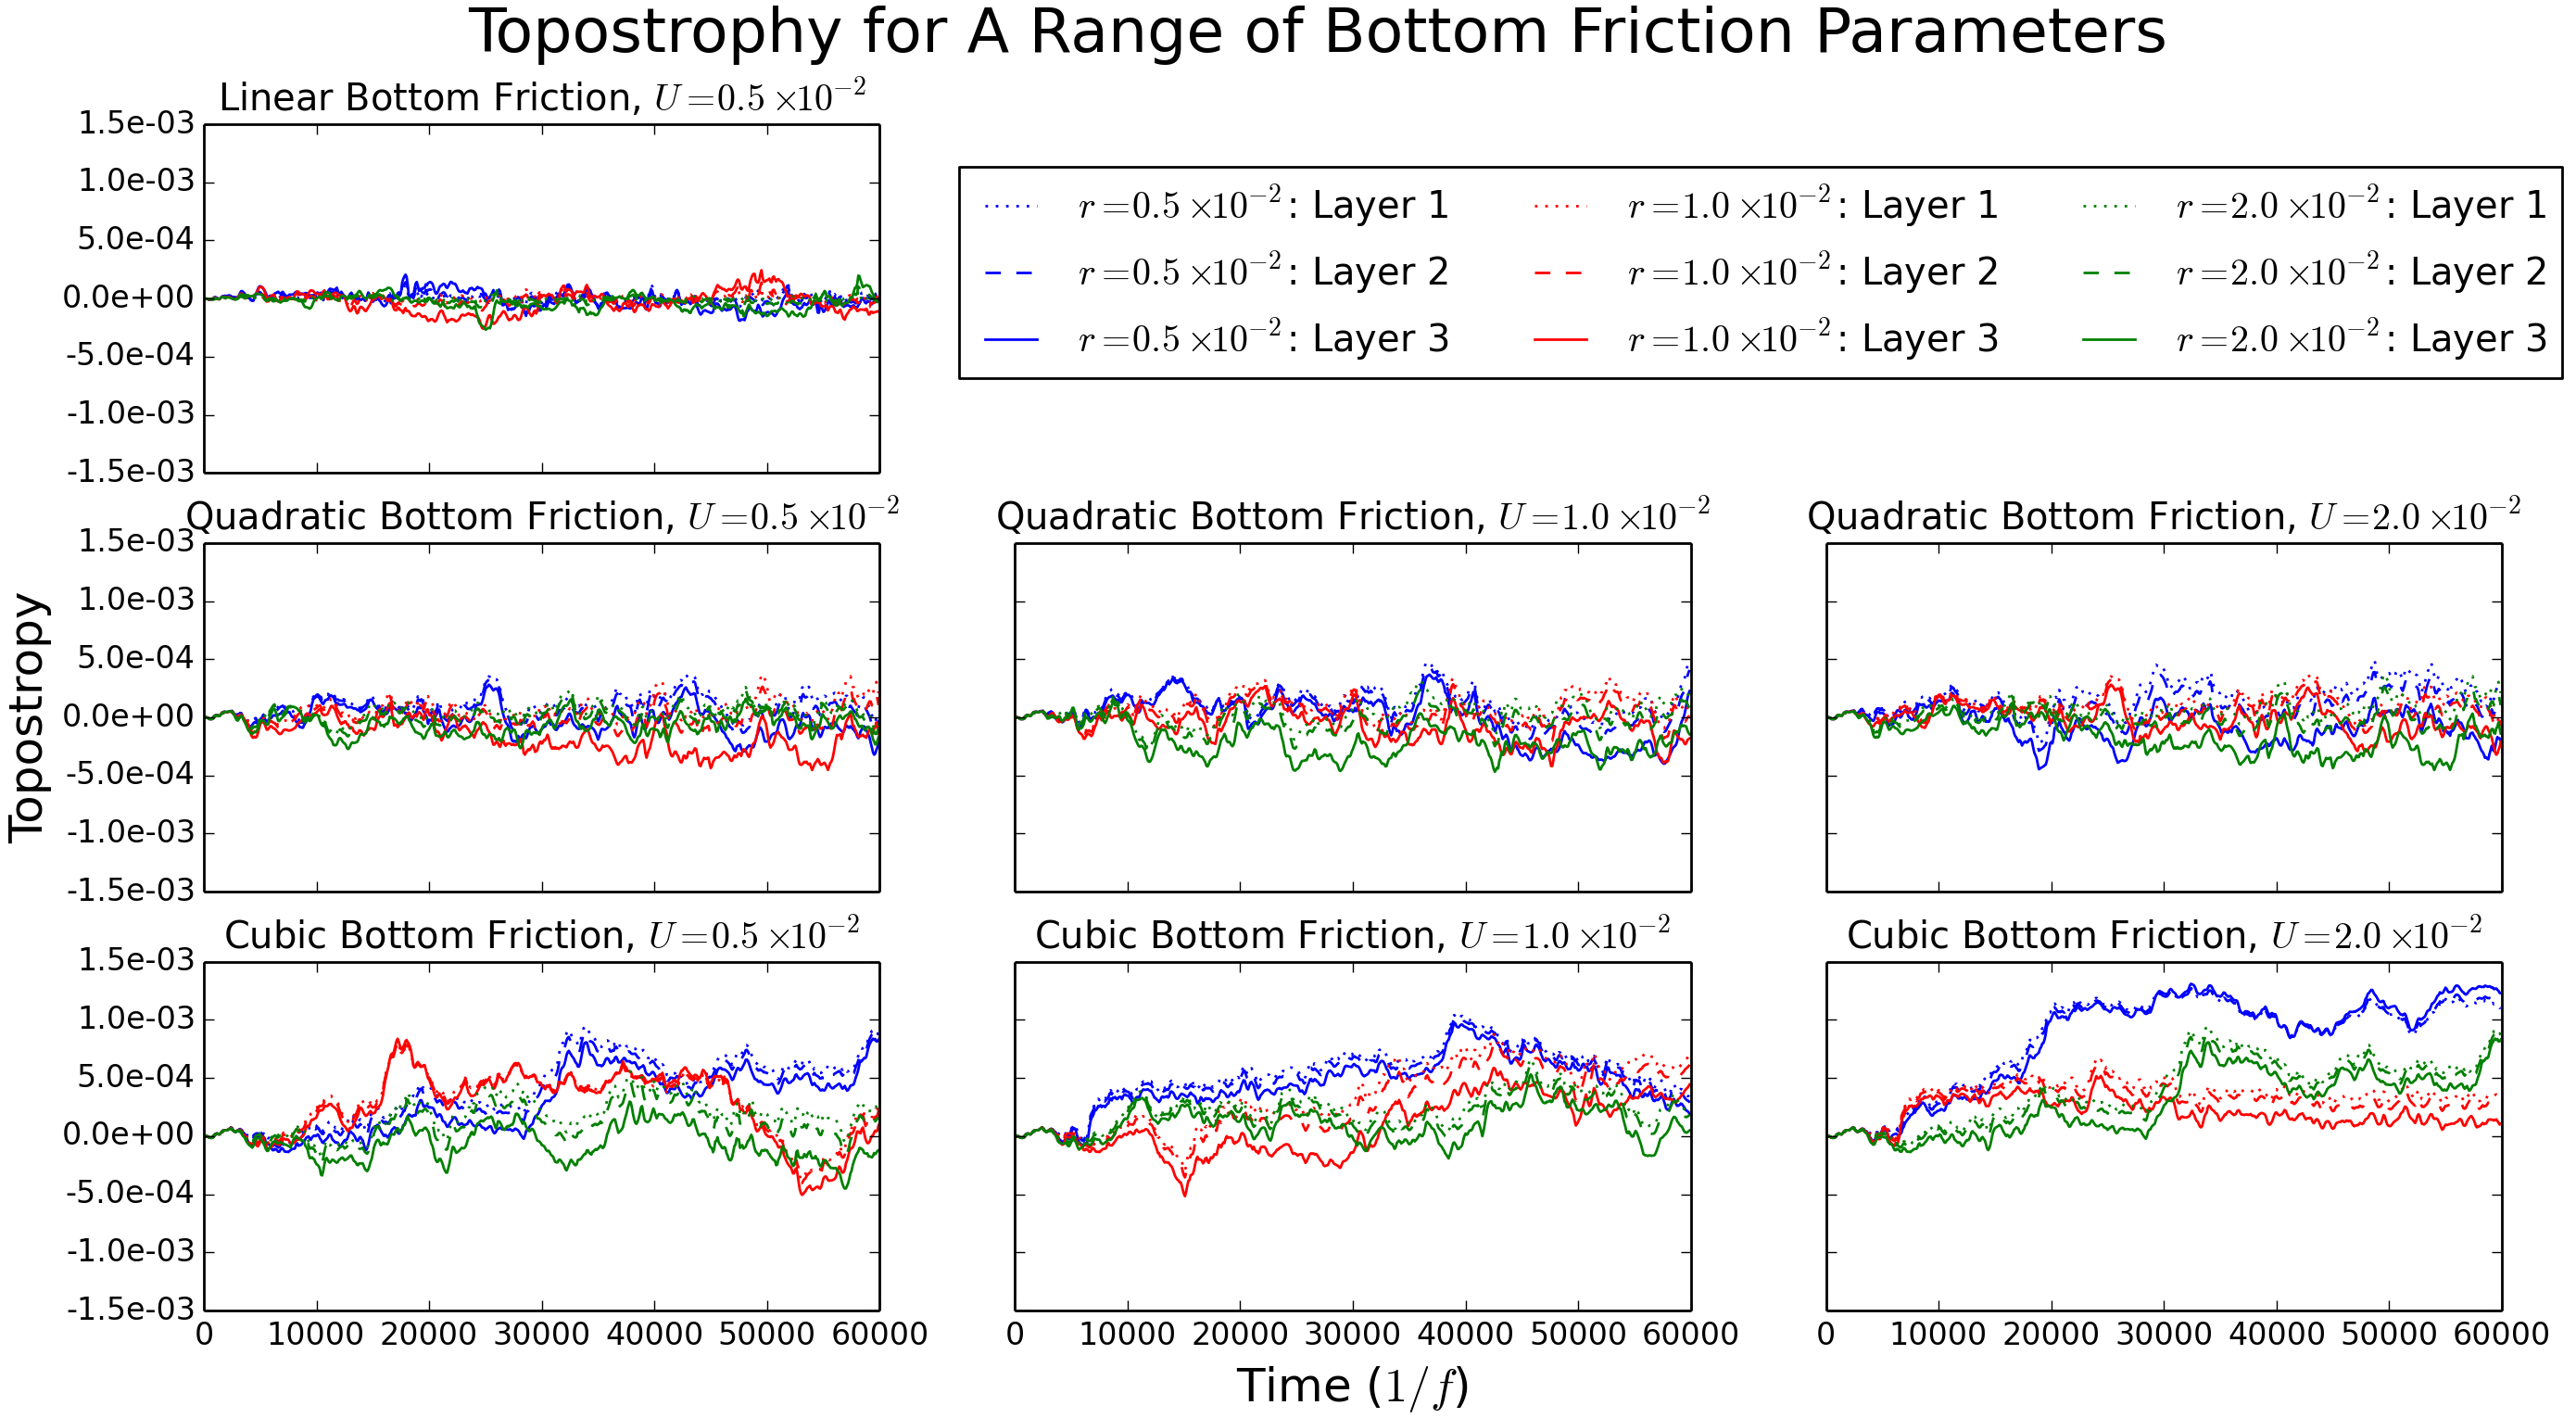
\includegraphics[width=\linewidth]{topostrophy}
  	\caption{Topostrophy for a range of different bottom friction parameters.
  		Each plot shows a certain choice of  $\left|\boldsymbol{u}^{\ast}\right|$
  		and $n$, with three different friction coefficients shown in red, green and blue.
  		The topostrophies calculated from the velocities in layers 1, 2 and 3 in each model
  		are shown by dotted, dashed and solid line respectively. Since 
  		$\left|\boldsymbol{u}^{\ast}\right|$ is non-existent in the linear case only
  		one plot is needed. }
  	\label{fig:topostrophy}
  \end{figure}
  
  In summary, we have created a model that is simple and quick, but still is a
  reasonable representation of the ocean. Using this model, we can apply 
  averaging operators to diagnose eddy-mean interactions in the 
  presence of topography using the theory developed
  in \secref{eddymeantheory}. However, before we get to topography, let us convince
  ourselves that we have a model that is consistent the equations derived in
  Chapter~\ref{sweq} and our conception of ocean dynamics. 
  Using the wind stress that we will discuss in detail in \secref{stochwind} in
  a three-layered domain without topography we spin up a model to examine the 
  resulting eddy field and momentum and energy balances. 
  \equref{swlayercorrectenergy} demonstrates a definition of energy that is conserved 
  except for forcing and dissipation, in this case this is the wind stress, bottom 
  friction and viscosity. \figref{fig:notopenergy} demonstrates that 
  the bottom friction balances the energy input from the wind over a large time
  window beyond the initial spin up. \figref{fig:notoppv} shows a snapshot of the \gls{pv}
  field around $40 \times 10^{3}/f$ into the run. The surface layer shows a strong eddy
  field with eddies around the scale of the deformation radius and some filamentation.
  The middle layer has basically uniform \gls{pv} as one would expect since 
  the only non-conservative term in the \gls{pv} equation for this layer is the
  viscosity, which is small. In the lowest layer the eddy field is mostly dissipated
  by the bottom friction, which is scale selective for strong flows leaving only shallow
  \gls{pv} gradients. This means there is slow and large scale barotropic flow
  present in all layers which whose magnitude is set by the bottom friction and spacial
  scale appears to be set by the domain size, whilst in there is a strong eddying 
  baroclinic flow whose spatial scale is set by the first baroclinic deformation radius
  and strength is set by the wind. In the time averaged mean, the variations of the
   \gls{pv} from the mean $f/h_{n}$ are vanishingly small, as shown in \figref{fig:notopmeanpv}, where with an averaging window of around $30 \times 10^{3}/f$
   the time-mean \gls{pv} varies by around $10 \%$ of the variability of the snapshot 
   \gls{pv} in \figref{fig:notoppv} whilst the time-mean flow speed is around $5 \%$.
  
  
  
  \begin{figure}
  	\centering
  	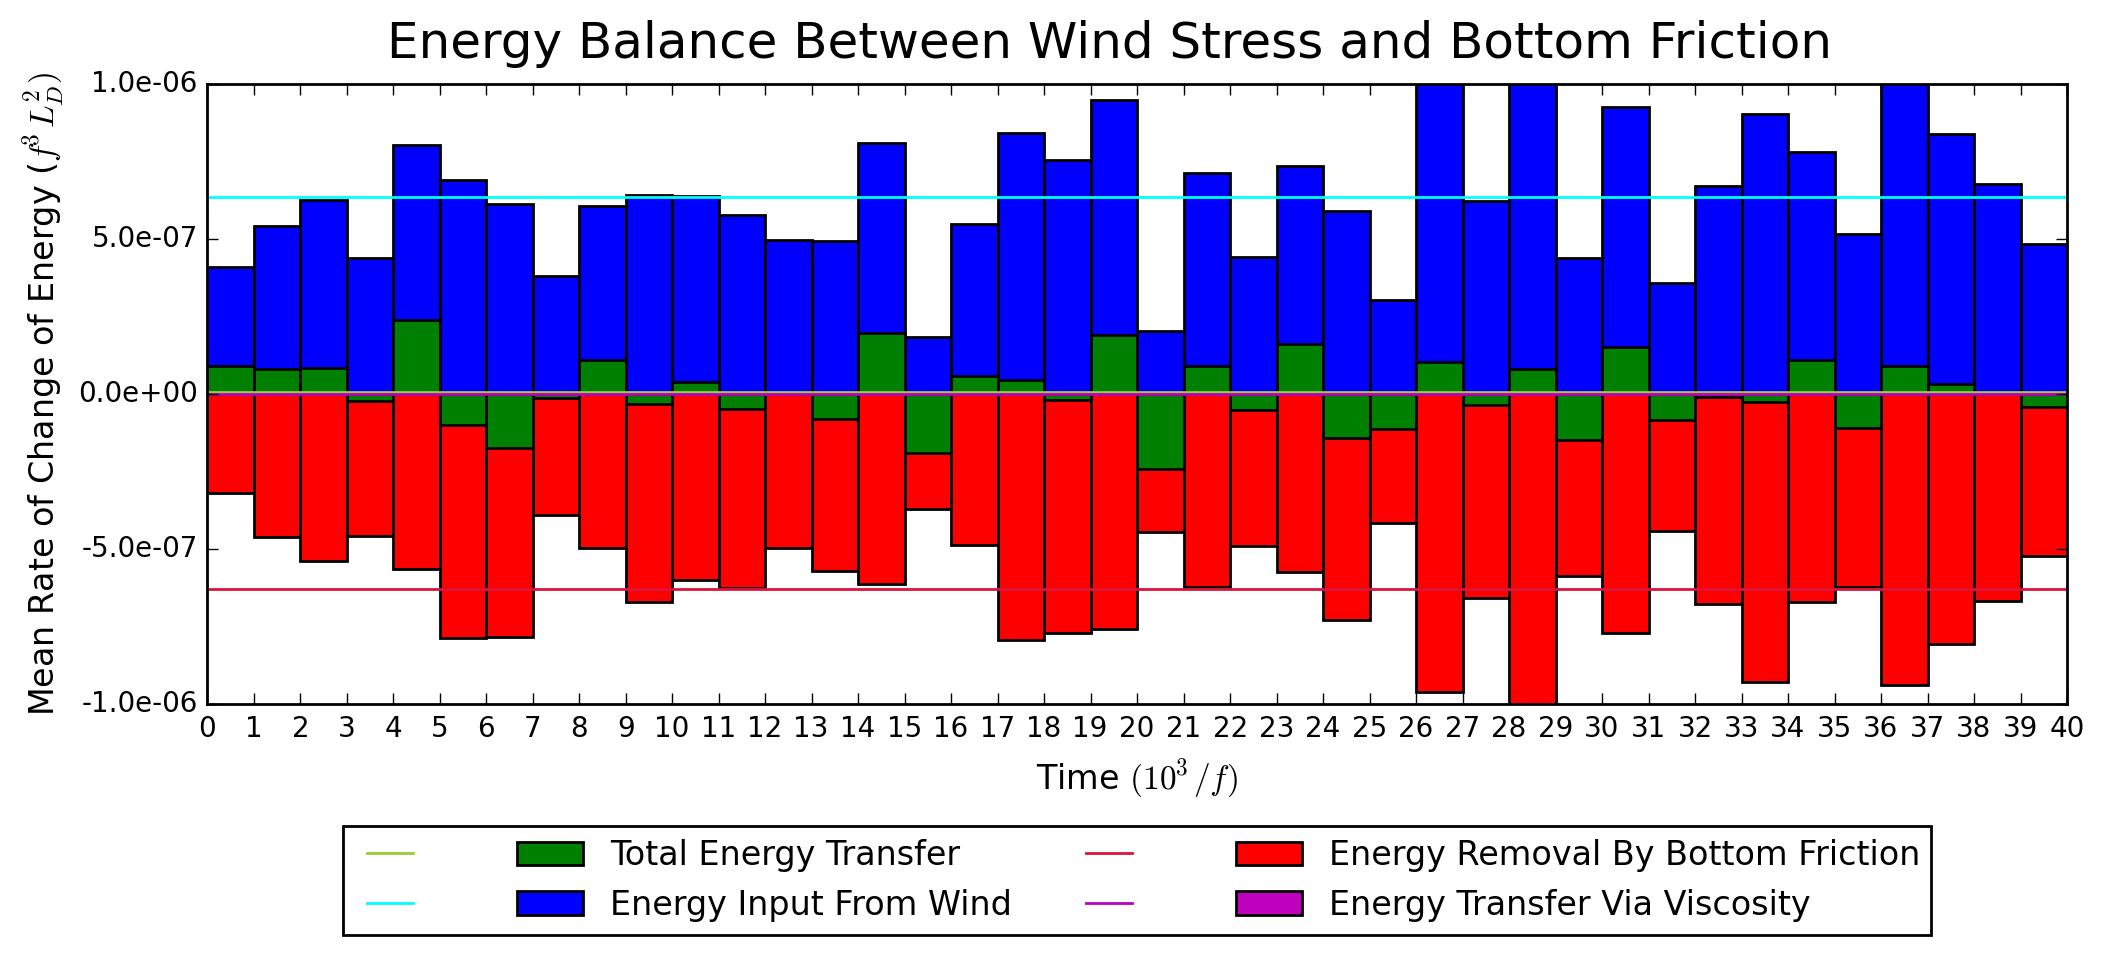
\includegraphics[width=\linewidth]{notopenergy}
  	\caption{Energy change in topography-less model represented by mean rate of change of energy per unit column over $10^{3}/f$ time window. Energy transfer is split into 
  		energy input by wind stress (\textcolor{blue}{blue}), dissipation through bottom friction (\textcolor{red}{red}) and transfer to small scale through the viscosity
  		(\textcolor{magenta}{magenta}), where the viscosity is negligible. The sum of these
  		is are the \textcolor{green}{green} bars. The lines are the mean transfers over the whole time window for wind stress, bottom friction, viscosity and total (\textcolor{blue}{blue}, \textcolor{red}{red}, \textcolor{magenta}{magenta} and \textcolor{green}{green} respectively). The overall energy transfer is about $1\%$
  		of the wind input and friction dissipation but is vanishingly small when the first
  		few averaging windows are excluded, i.e. the spin up period.}
  	\label{fig:notopenergy}
  \end{figure}
  
  
  
  \begin{figure}
  	\centering
  	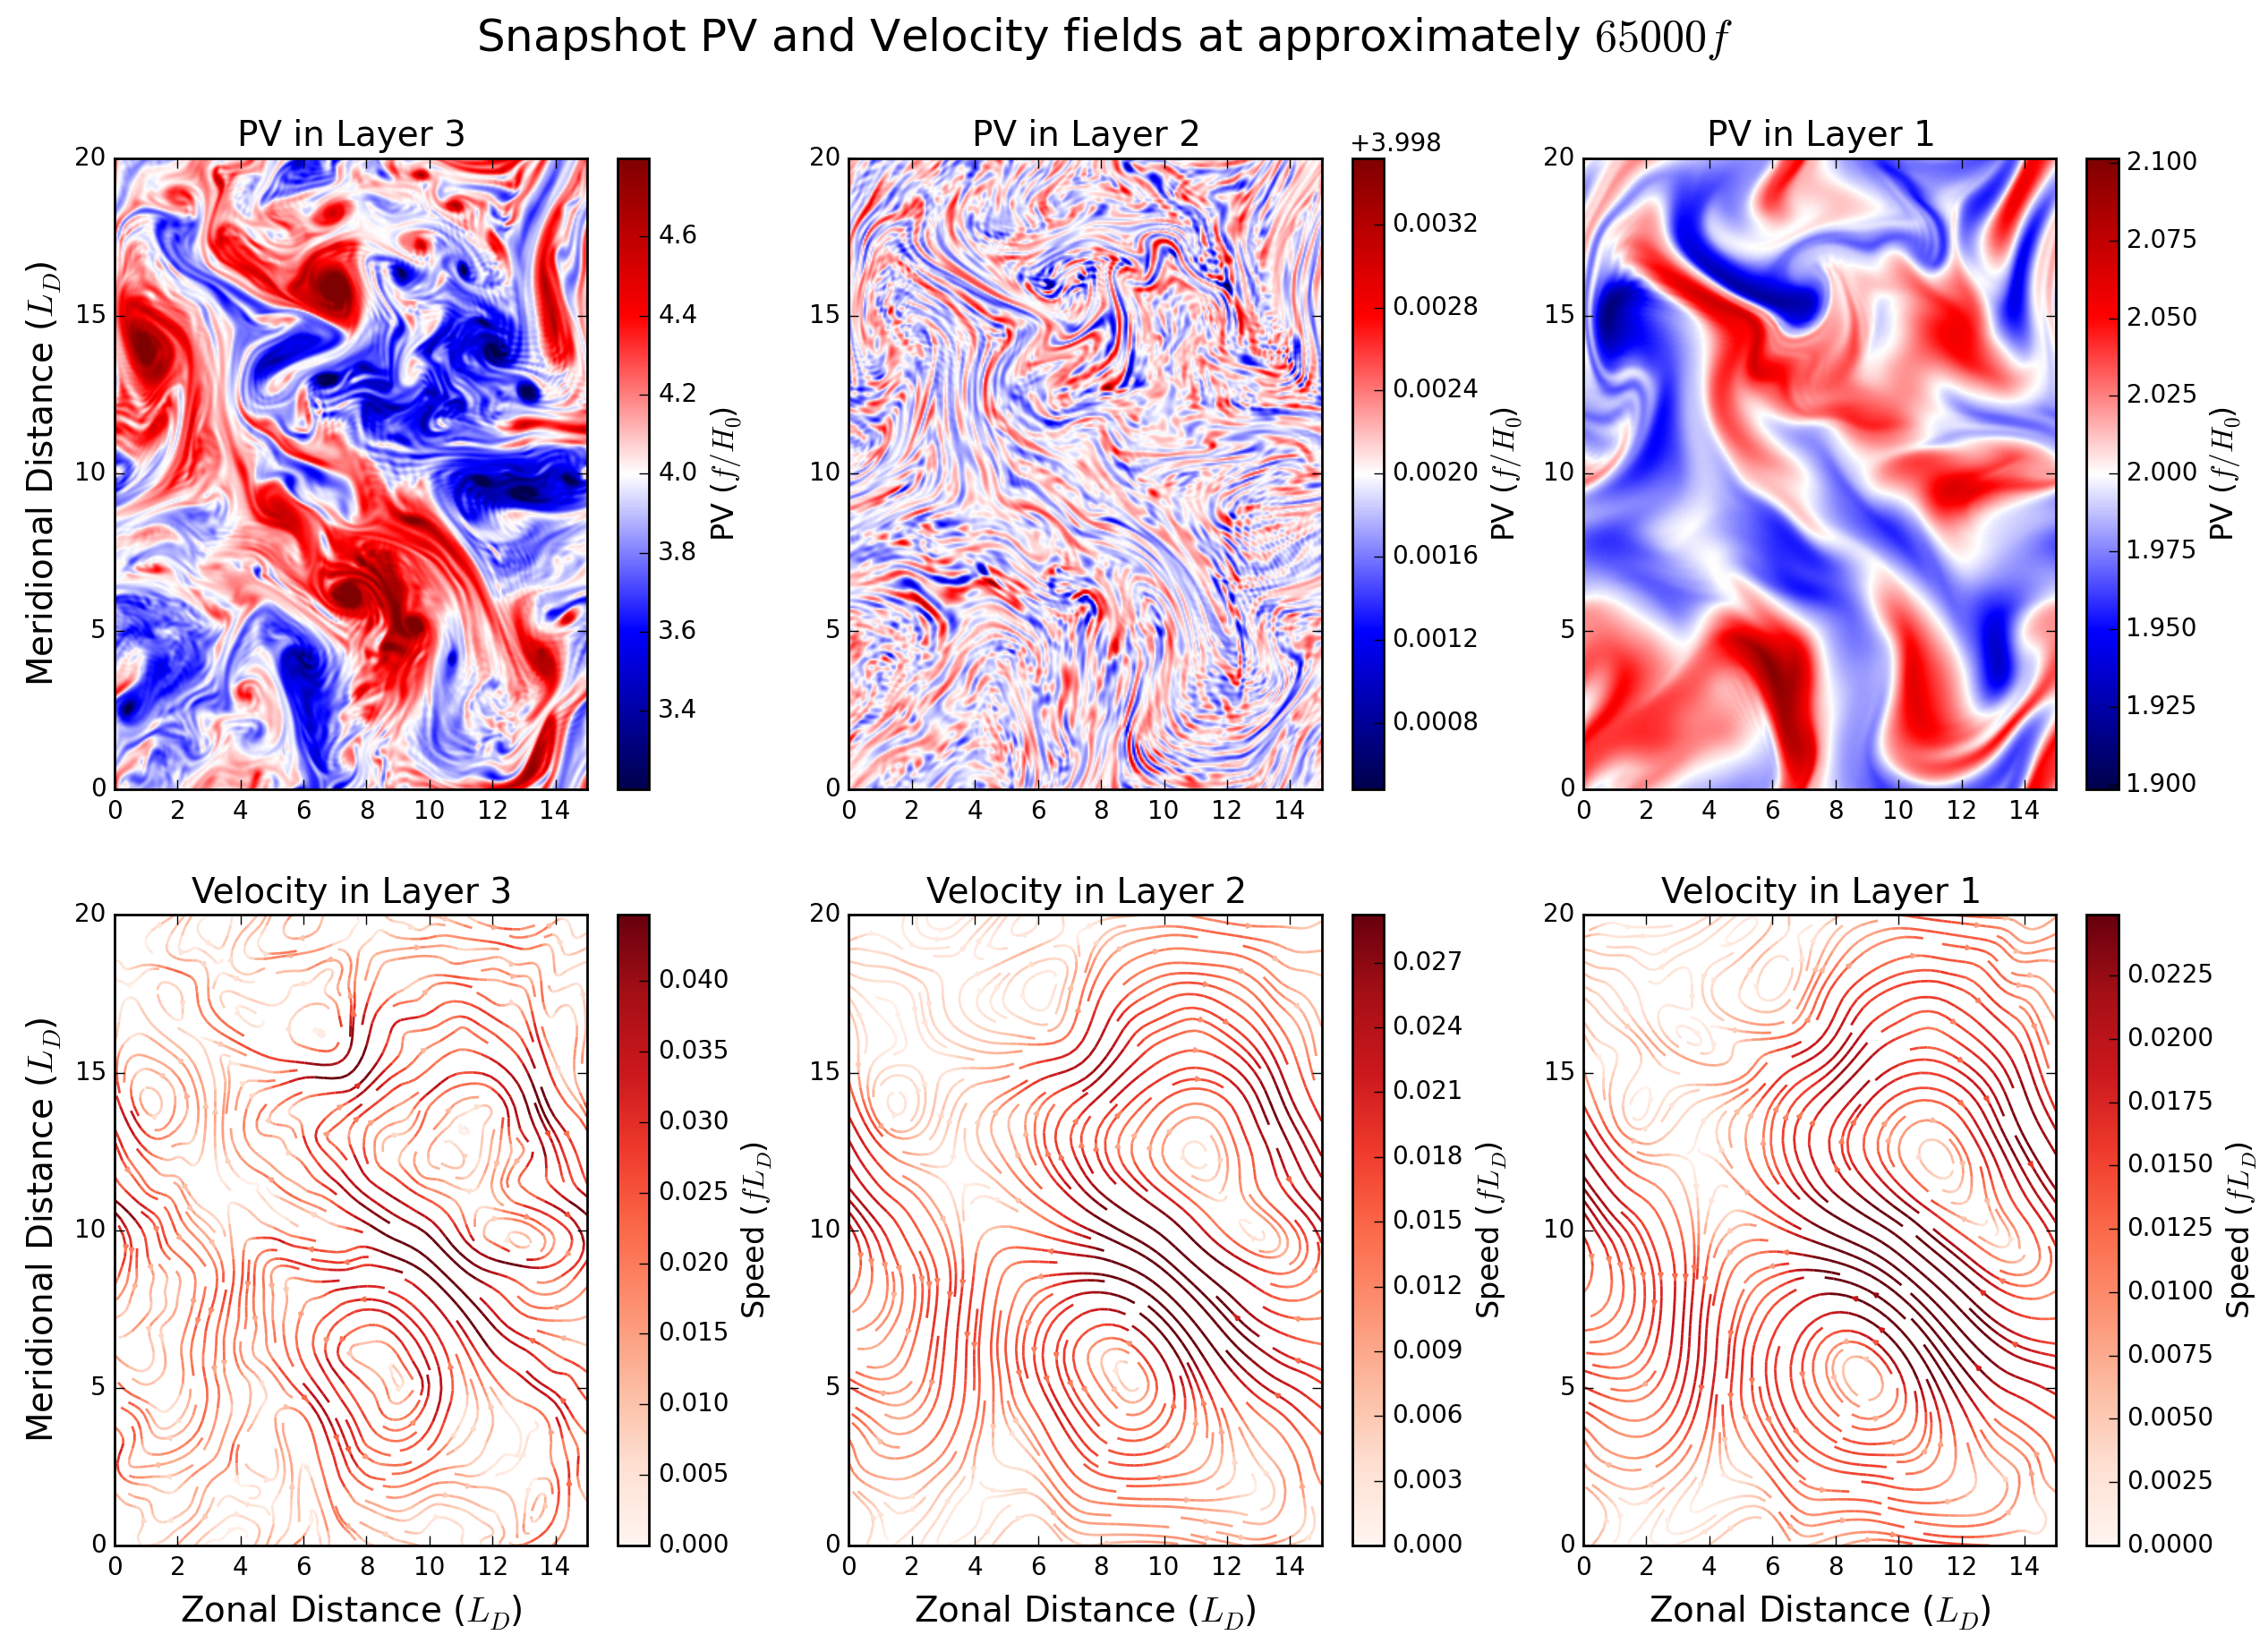
\includegraphics[width=0.8\linewidth]{notoppv}
  	\caption{}
  	\label{fig:notoppv}
  \end{figure}
  
  
  \begin{figure}
  	\centering
  	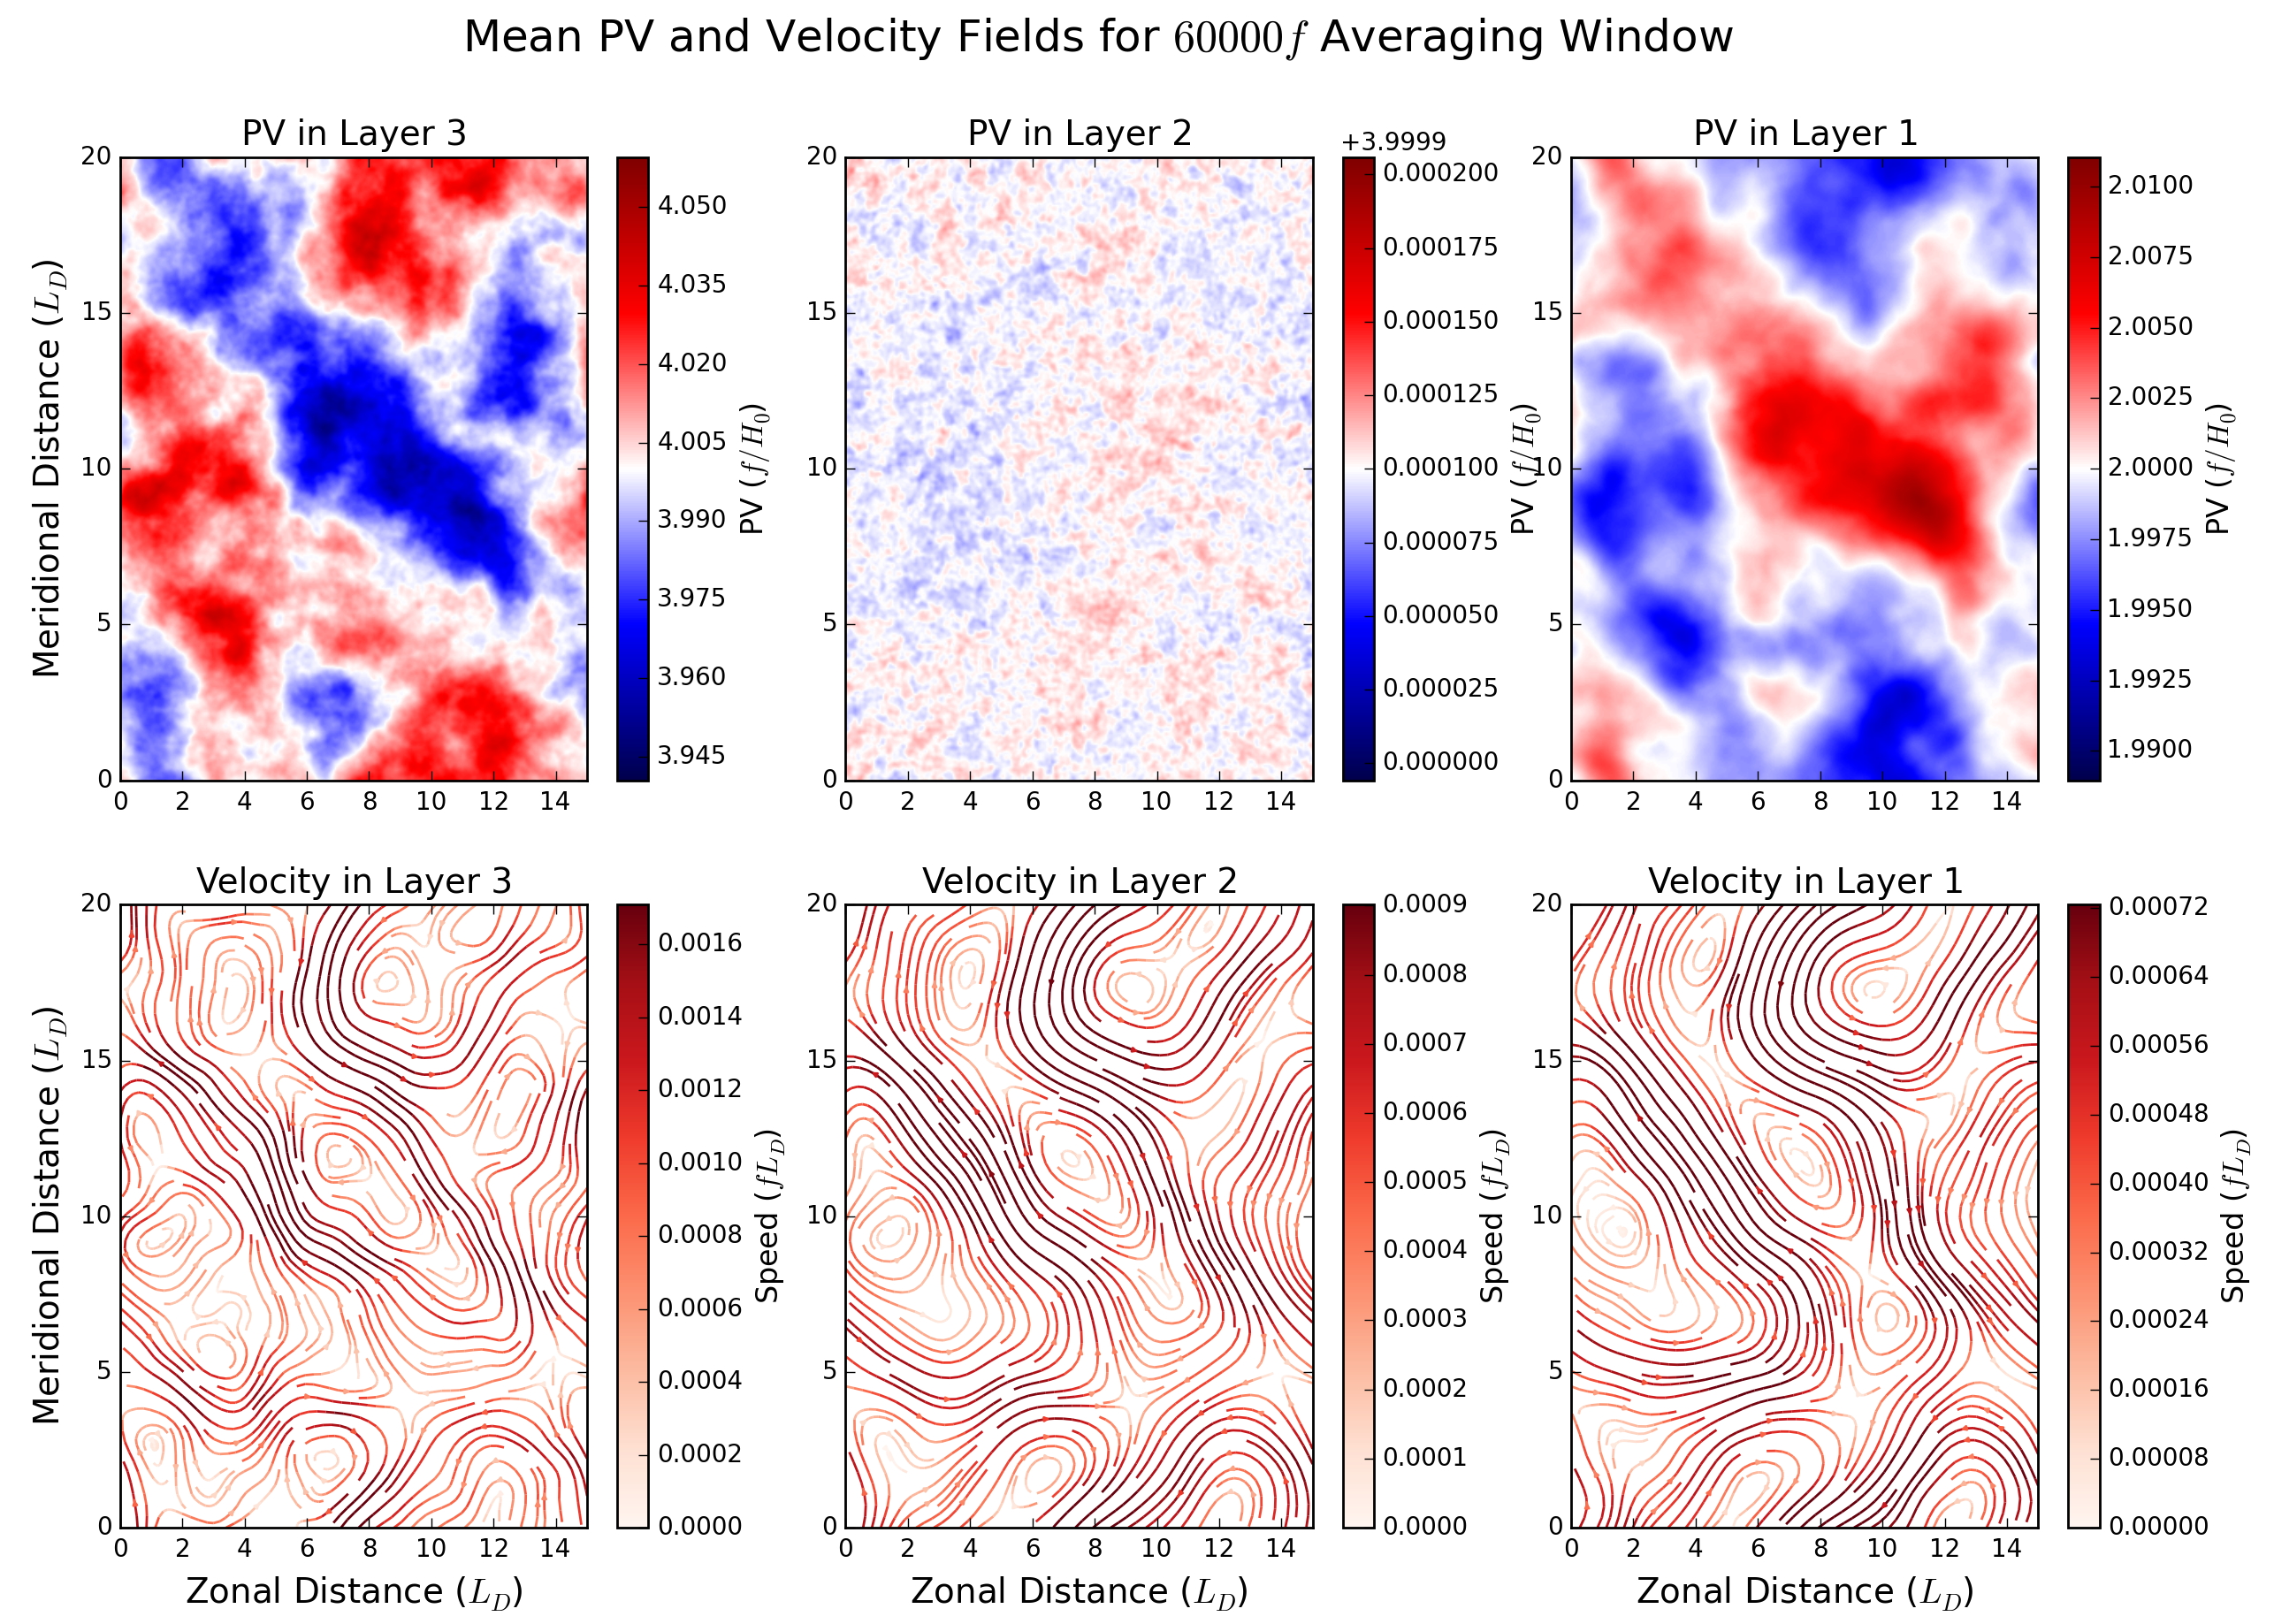
\includegraphics[width=0.8\linewidth]{notopmeanpv}
  	\caption{}
  	\label{fig:notopmeanpv}
  \end{figure}


\chapter{Analysis of a hierarchy of models}

Now that we have system that suits the needs that we outlined in the
introduction of Chapter~\ref{sweq} we can proceed with investigating the
role of mean-eddy flow interaction in the presence of topography.
As mentioned in the previous section, due choosing to have a doubly re-entrant
domain the choice of topography must be zonally and meridionally translationally symmetric.
Hence, we choose to have a zonal ridge as shown in the schematics
 \figref{fig:TopographySchem} as well as \figref{fig:TopographyCross}, which
 depicts a cross-section of the initial configuration of the domain where
 the layer thicknesses are chosen in such a way as to attempt reduce the chance of a
 layer outcropping by evenly distributing the layers above shallowest topography. Our
 understanding of eddy-topography interactions build from observational 
 data and experiments that were outlined in Chapter~\ref{intro} would lead us
 to expect an along topography flow to develop with an westward flow on the south side of
 the ridge, and an eastward flow on the north side of the ridge for a positive $f_{0}$.



\begin{figure}
	\centering
	\begin{minipage}[b]{0.45\linewidth}
		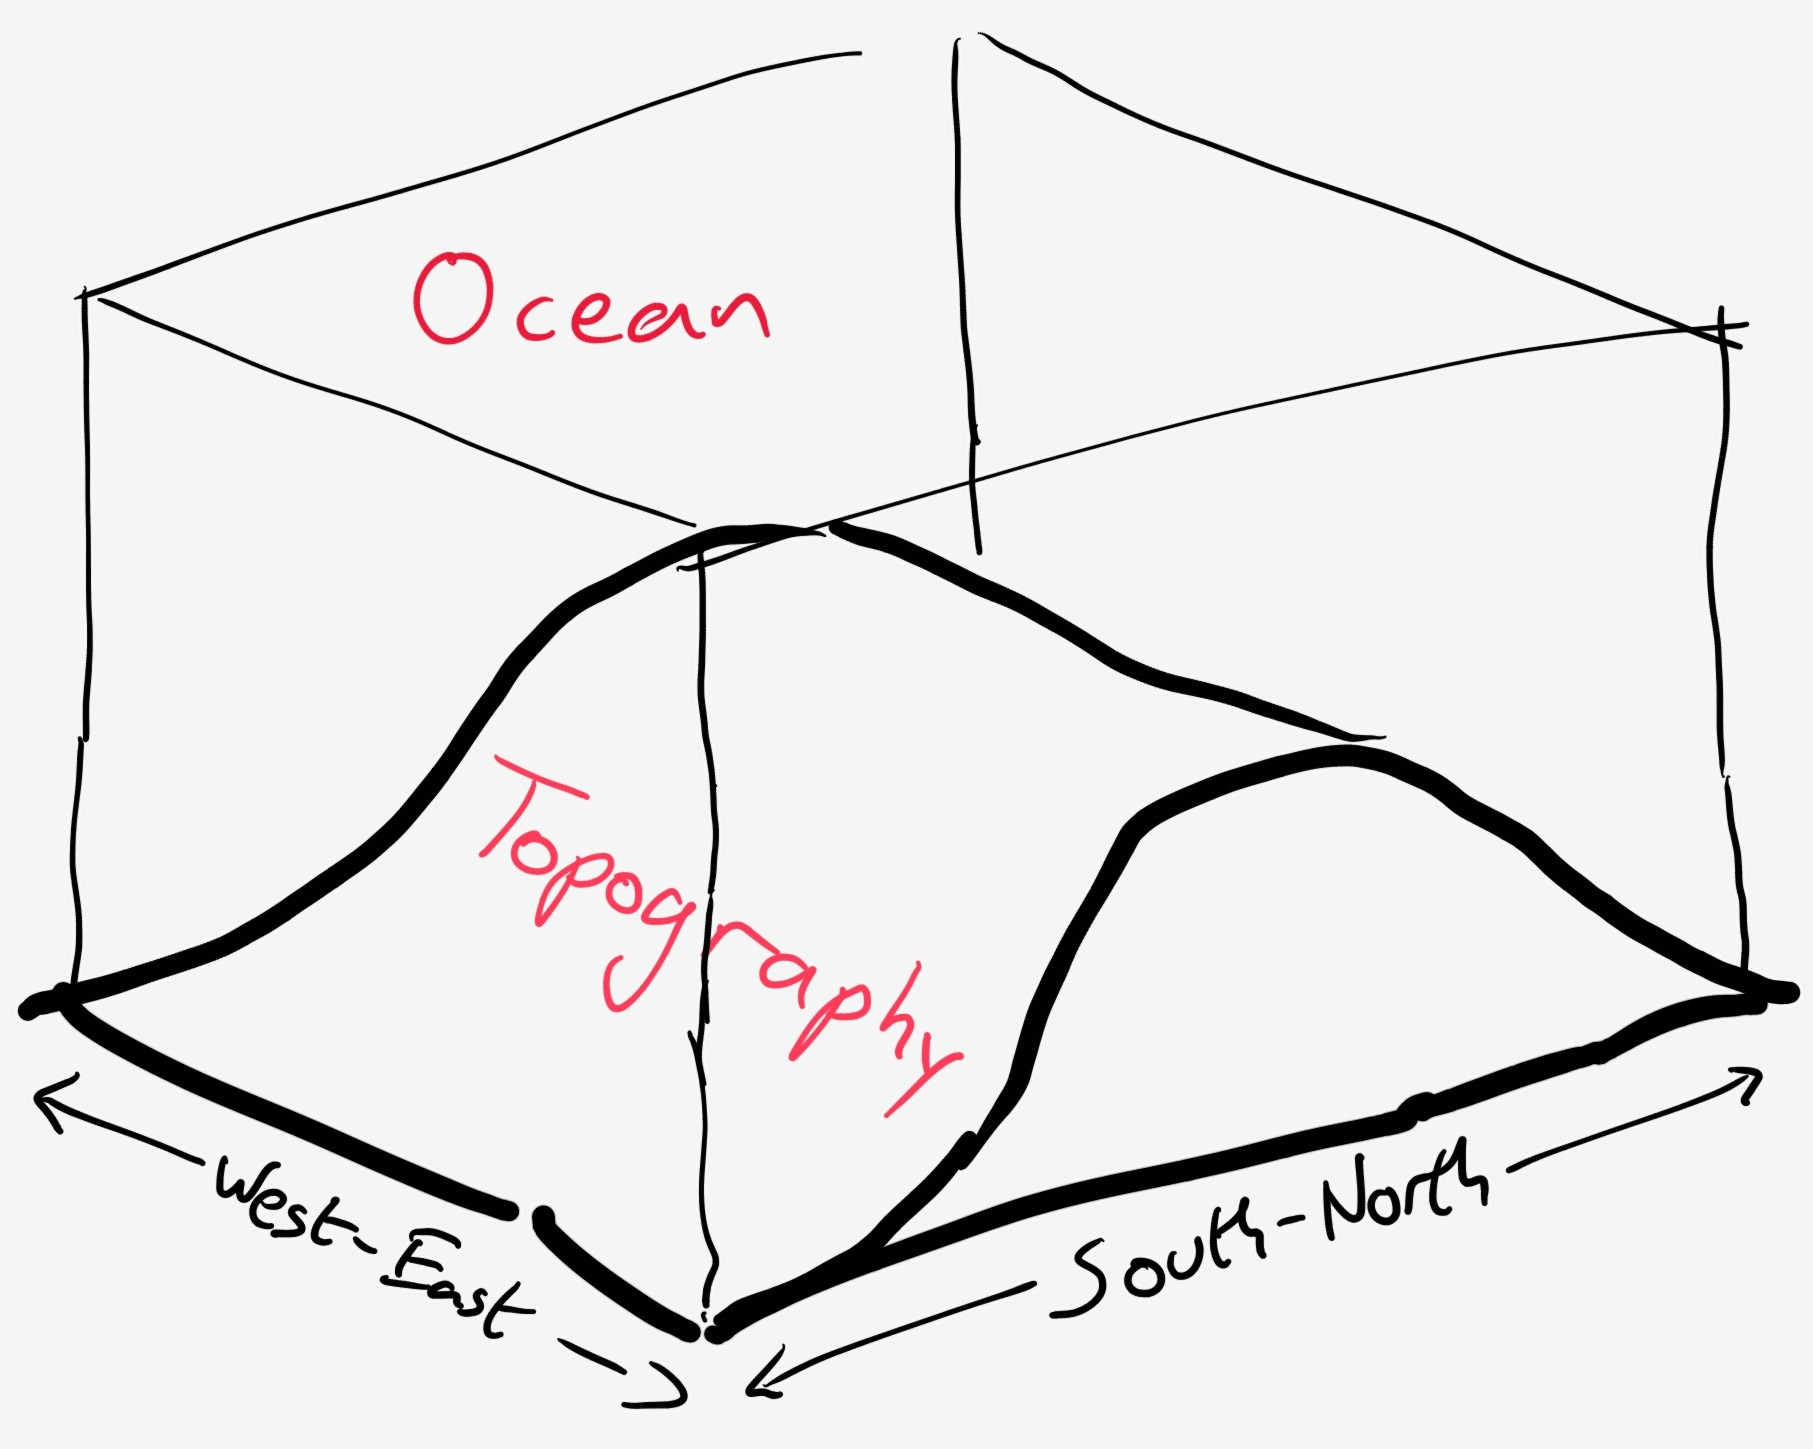
\includegraphics[width=\linewidth]{Topography}
		\caption{Schematic of the topography. The dimensions of the domain
			are $10 L_{D}$ in the direction along the 
			ridge, where $L_{D}$ the deformation
			radius defined in the text, and $15 L_{D}$ 
			in the perpendicular direction. }
		\label{fig:TopographySchem}
	\end{minipage}
	\quad
	\begin{minipage}[b]{0.45\linewidth}
		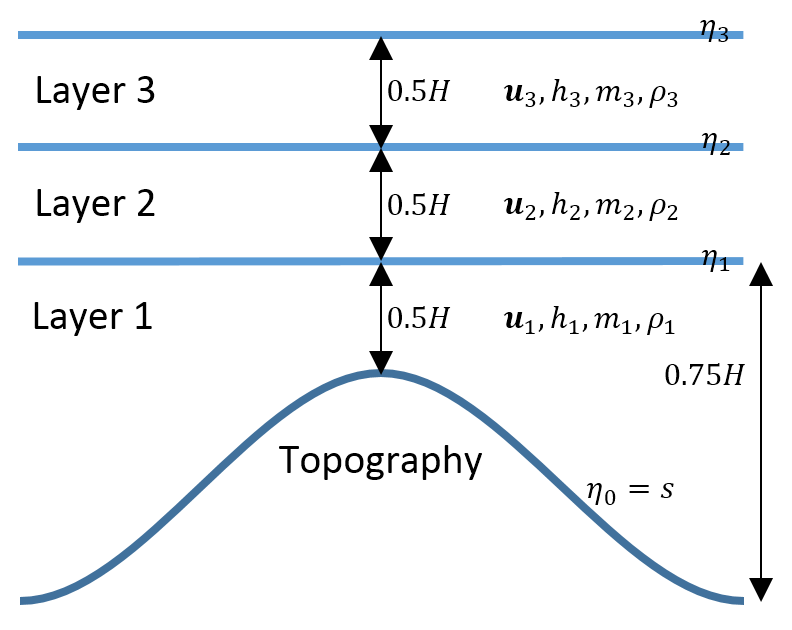
\includegraphics[width=\linewidth]{TopographyCross}
		\caption{ Cross-sectional schematic of the topography. 
			Shows three layers of fluid, with densities 
			$\rho_{1}$, $\rho_{2}$ and $\rho_{3}$, above the 
			topography, $s$. Interfaces between individual
			layers, the surface and topography are labelled $\eta_{i}$ for
			the interface above layer '$i$' and  $\eta_{0}=s$. }
		\label{fig:TopographyCross}
	\end{minipage}
\end{figure}

%A description of the different dynamics that evolve
%in the models by using the forcings and 
%dissipations described above. Different forcings
%such as different wind stresses or regional heating
%and cooling. Different dissipation from
%linear bottom friction to higher order bottom
%friction.

%Break down of the tendency terms for the mean
%dynamics. A look at how the eddy stresses are 
%in balancing the mean states (usually through
%balancing the ageostropic component of the
%momentum tendency).

%A closer look at the eddy stress, their bounds 
%and the available eddy budgets.

\section{Zero-Mean Wind Stress}

\label{stochwind}

To begin, it seems most sensible to investigate the 
system with the simplest possible mean dynamics.
That is to say a system where the dynamical equations 
for the mean variables (for example \equref{swtwaeqs}) is 
only forced by the eddy-mean interaction and dissipation,
for example bottom friction. Of course, if the mean system is
only forced by the eddy-mean interactions and dissipative forces
then they only way interesting dynamics can occur
is through the eddy-mean interactions. Hence, we try to
generate an eddy field from some kind of forcing such that in the mean 
dynamics there is no contribution from the forcing, that is to say
that for forcing, $\boldsymbol{\tau}$, we have $\thkmean{\boldsymbol{\tau}}\equiv0$.


To achieve such a system we introduce a spatially and temporally 
varying wind stress. There are a few  way this can be done, a common method
is to generate a superposition of sine waves at various frequencies and 
phases as the stream function for the wind stress, this method is discussed at
length in \cite{brannigan2015seasonal} and \cite{koszalka2009dynamics}. 
Instead we populate the domain
with a collection of cyclones and       anticyclones. These, we define
in such a way that they each  independently give a circular wind
stress of a curtain maximum amplitude and that is vanishing small far from its centre,
with a continuous stream function      and curl. The profile shown in 
Figure~\ref{fig:WindEg}
satisfies these conditions. It has five properties which can be altered to 
create a stress field which can be implemented in the model; these are it's
amplitude, radius, position, duration and orientation (i.e. whether it is cyclonic
or anticyclonic). By periodically generating these vortices with randomised properties
we can sum them together to create a wind stress which varies in time, and in the limit
of a long run time, the time-mean sums to zero. Each individual cyclone or anticyclone
has the form $\frac{1}{2\pi r}(1-e^{-r^{2}})e^{-r^{2}/2}\boldsymbol{e}_{\theta}$, where
at the wrap around points half the domain away from the vortex centre the vortex is tapered
rapidly to zero to avoid a discontinuity; here $r$ is the distance from the centre of the vortex, normalised by the
radius of the vortex, and $\boldsymbol{e}_{\theta}$ is the unit vector in the 
rotational direction. The vortexes are also given a certain random duration, $t_{0}$, contained a minimum and maximum duration; the vortexes then
grow and decline over this period in proportion to a sign wave in the range $[0,\pi]$.
Examples of how the full wind stress field looks at different
time steps are shown in Figure~\ref{fig:StochWind}. To further ensure a vanishing
mean wind stress over a long time averaging window we introduce the vortexes in cyclonic
and anti-cyclonic pairs of equal size and duration to ensure that the spatial mean
of the wind stress is precisely zero. 

Now we must check that this wind stress satisfies our needs. 
The upper bound of momentum contribution from
this wind stress to the time-averaged mean system is straight forward to calculate
and is dependent on ratio between the longest $t_{0}$, or vortex duration, 
and the averaging window. So for similar wind stresses the contribution to the mean system
is vanishingly small for longer averaging windows. The energy input is a little more
complicated; the mean and eddy energy equations described in \secref{eddymeantheory} 
shows that applying the thickness weighted averaging operator to 
\hl{the energy equation (eq ref)} gives
$\nthkmean{\boldsymbol{\tau}}\cdot\nthkmean{\boldsymbol{u}}$ and  $\nthkmean{\nthkres{\boldsymbol{\tau}}\cdot\nthkres{\boldsymbol{u}}}$
as the energy input into the mean and eddy components of the system.
Taking averaging windows of $10^{3}/f$, \figref{fig:meaneddywind} shows
that the contribution to the mean component is vanishingly small 
and hence the wind stress suits our purpose by almost exclusively 
inputting energy and momentum into the eddy component of the system.

\begin{figure}
	\centering
	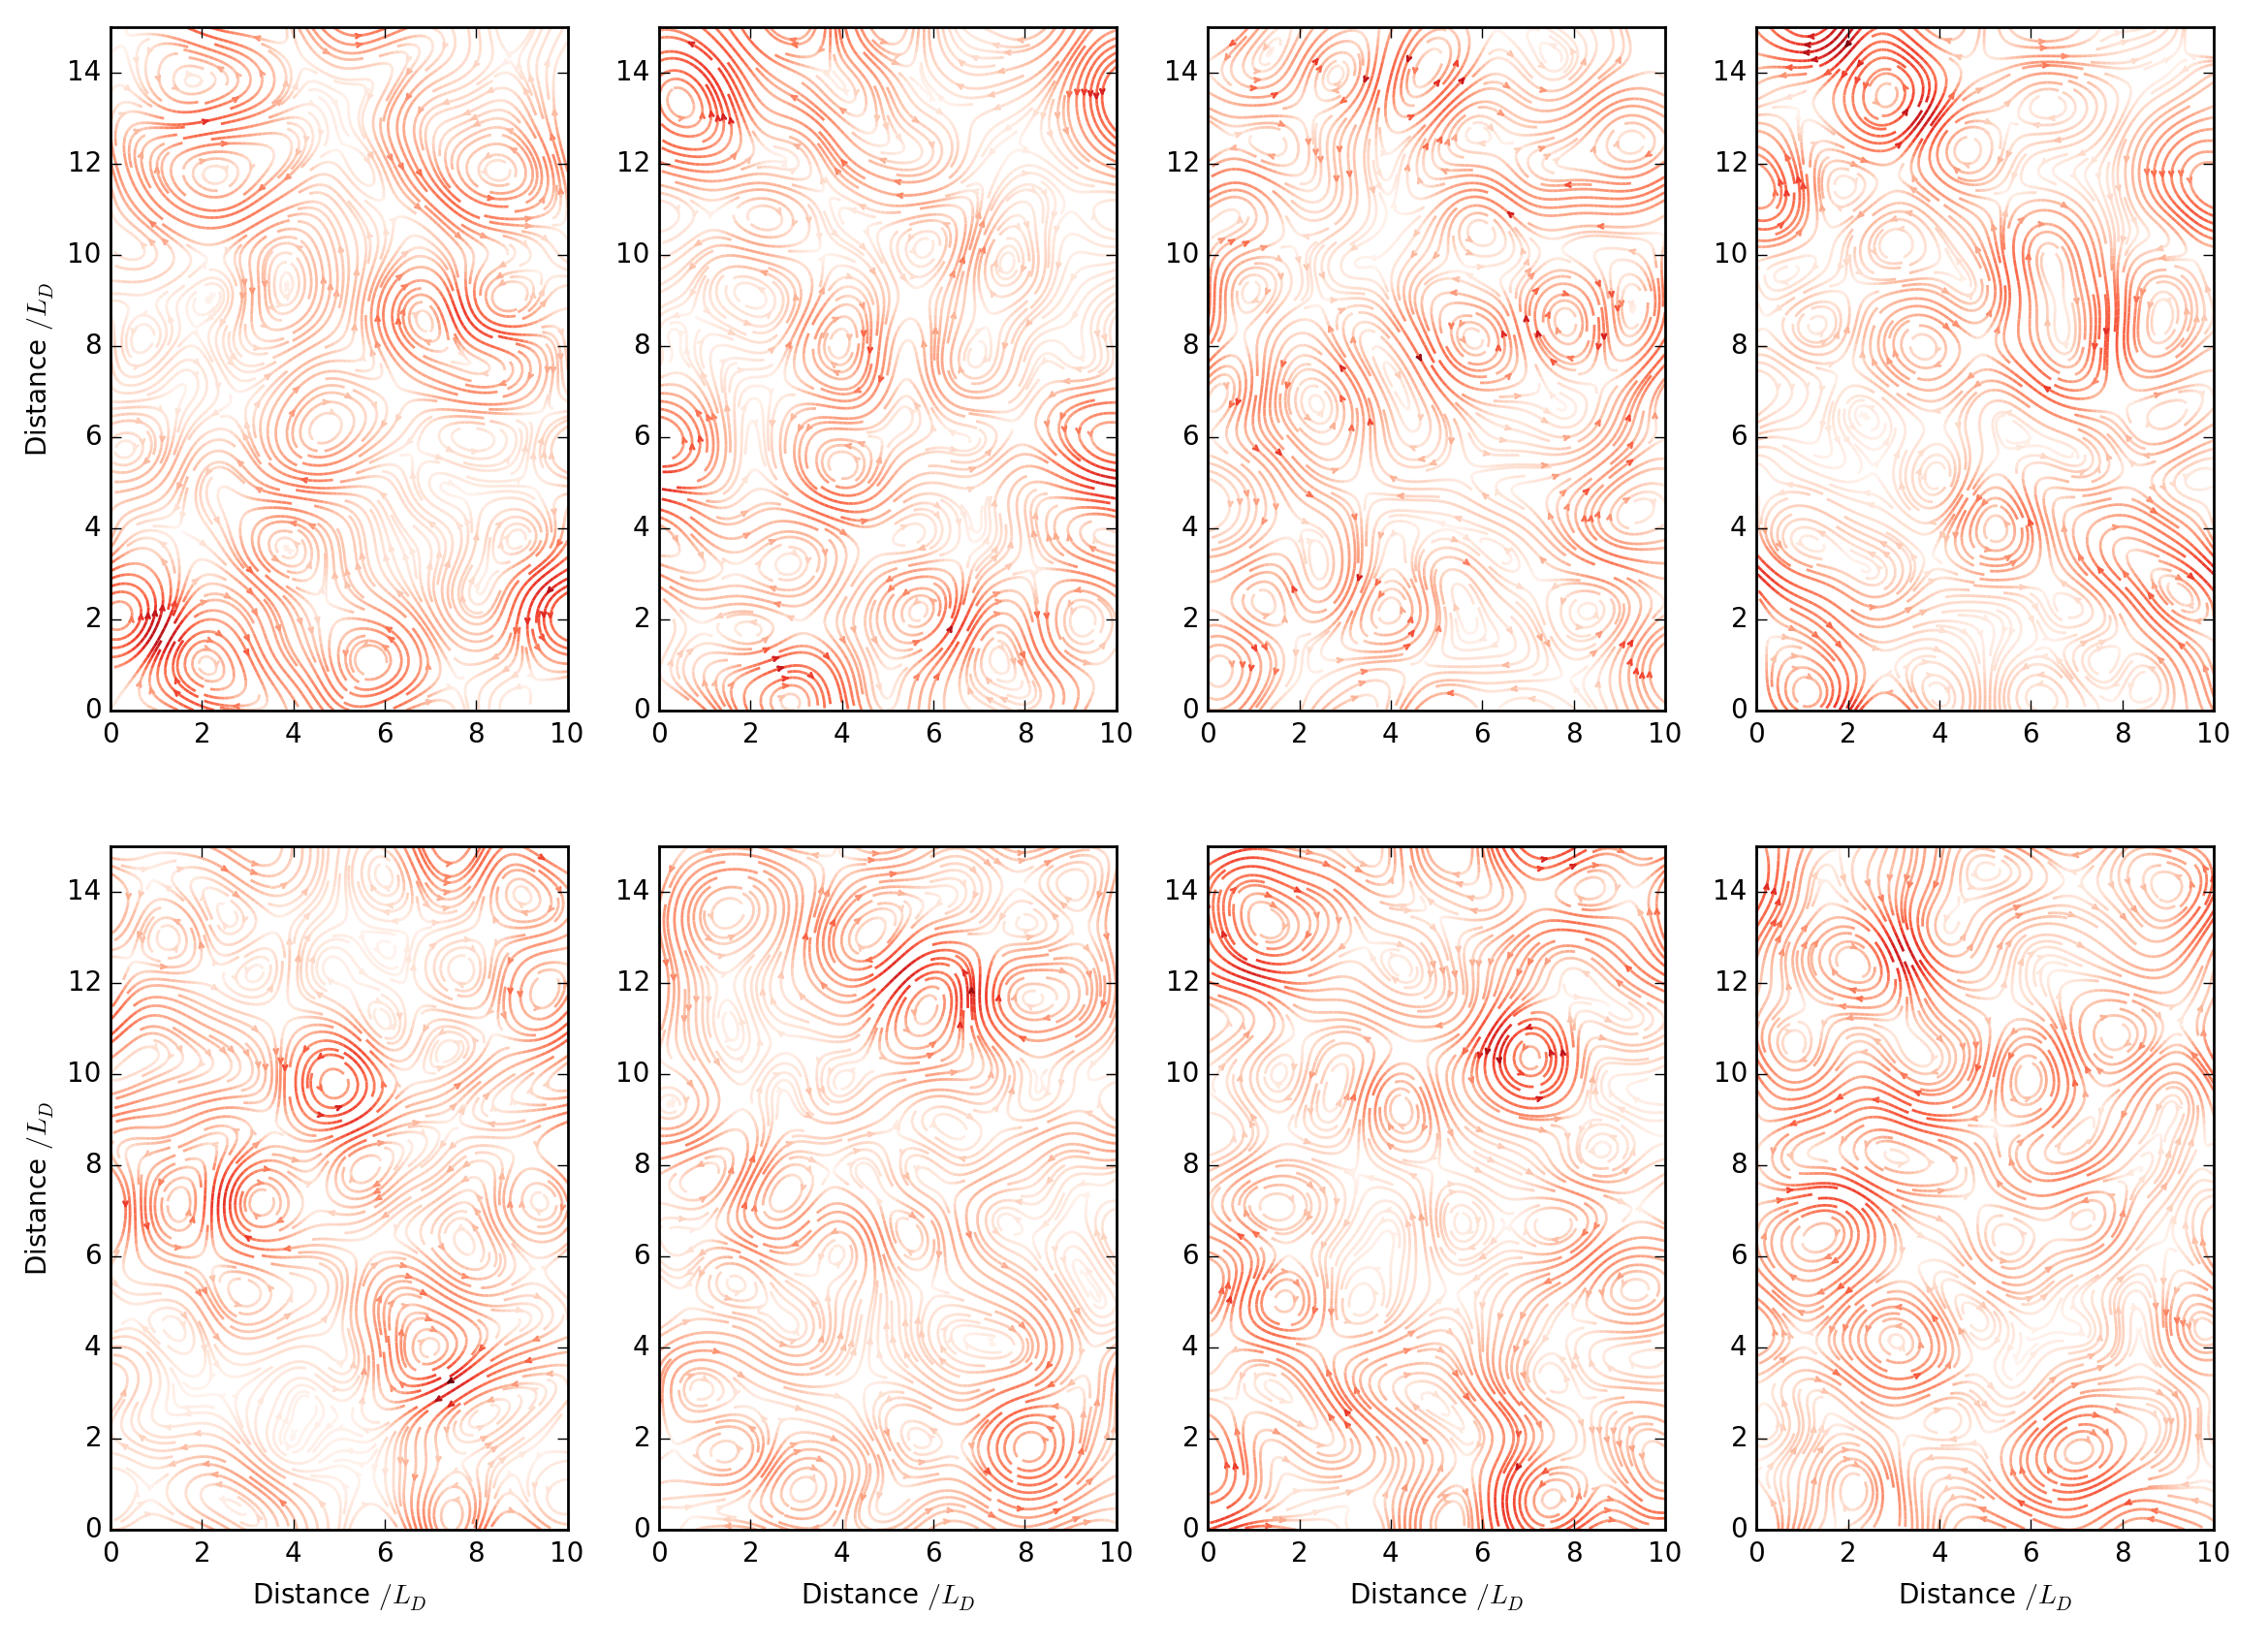
\includegraphics[width=\linewidth]{StochWind}
	\caption{\hl{not the actual snapshots, need to do redo this (notice the radii are wrong)} Eight different snapshots of the wind forcing
		generated by randomly seeding vortexes
		across the domain.
		These cyclones and anticyclones have a typical radii of between $5$ times
		the Deformation Radius and half the domain size, and have a lifespan of a couple of weeks}
	\label{fig:StochWind}
\end{figure}

\begin{figure}
	\centering
	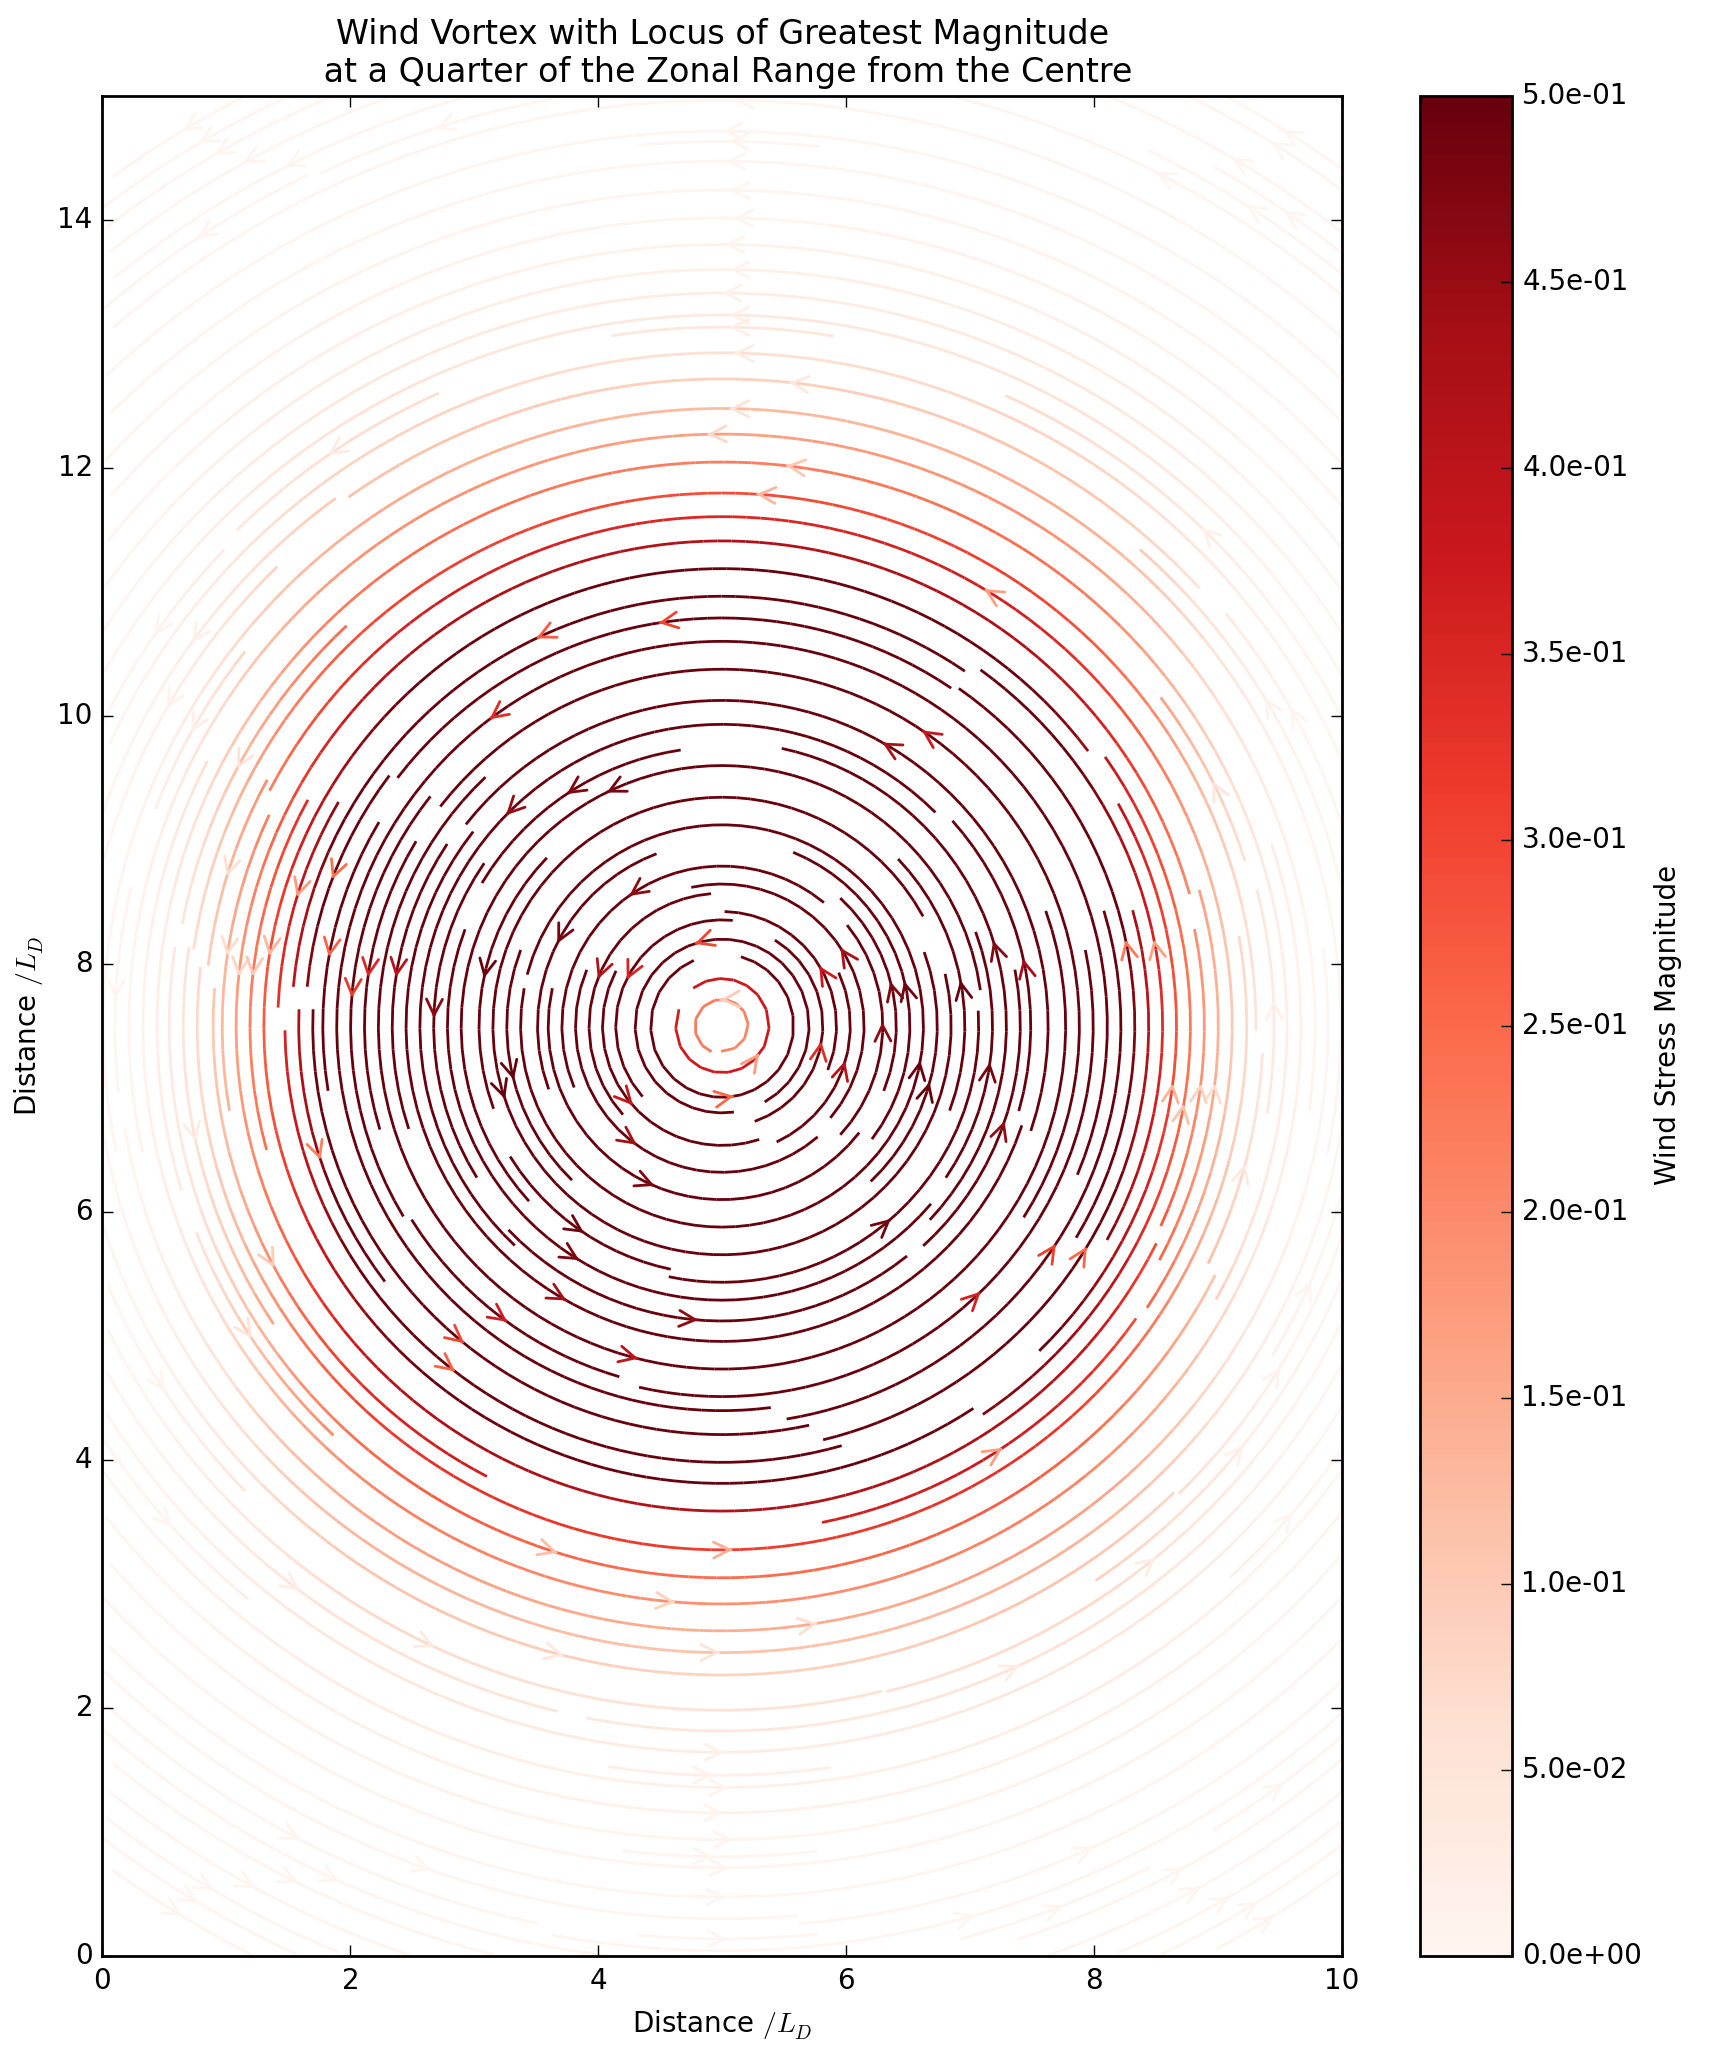
\includegraphics[width=\linewidth]{WindStressEg}
	\caption{\hl{also am going to redraw} An example of the wind stress given by a cyclone with
		radius a quarter of the zonal width of the domain. 
		The heat-map shows the strength of the stresses, 
		The  stresses are tapered away from the centre of the vortex to
		avoid discontinuities as the domain wraps around. }
	\label{fig:WindEg}
\end{figure}

\begin{figure}
	\centering
	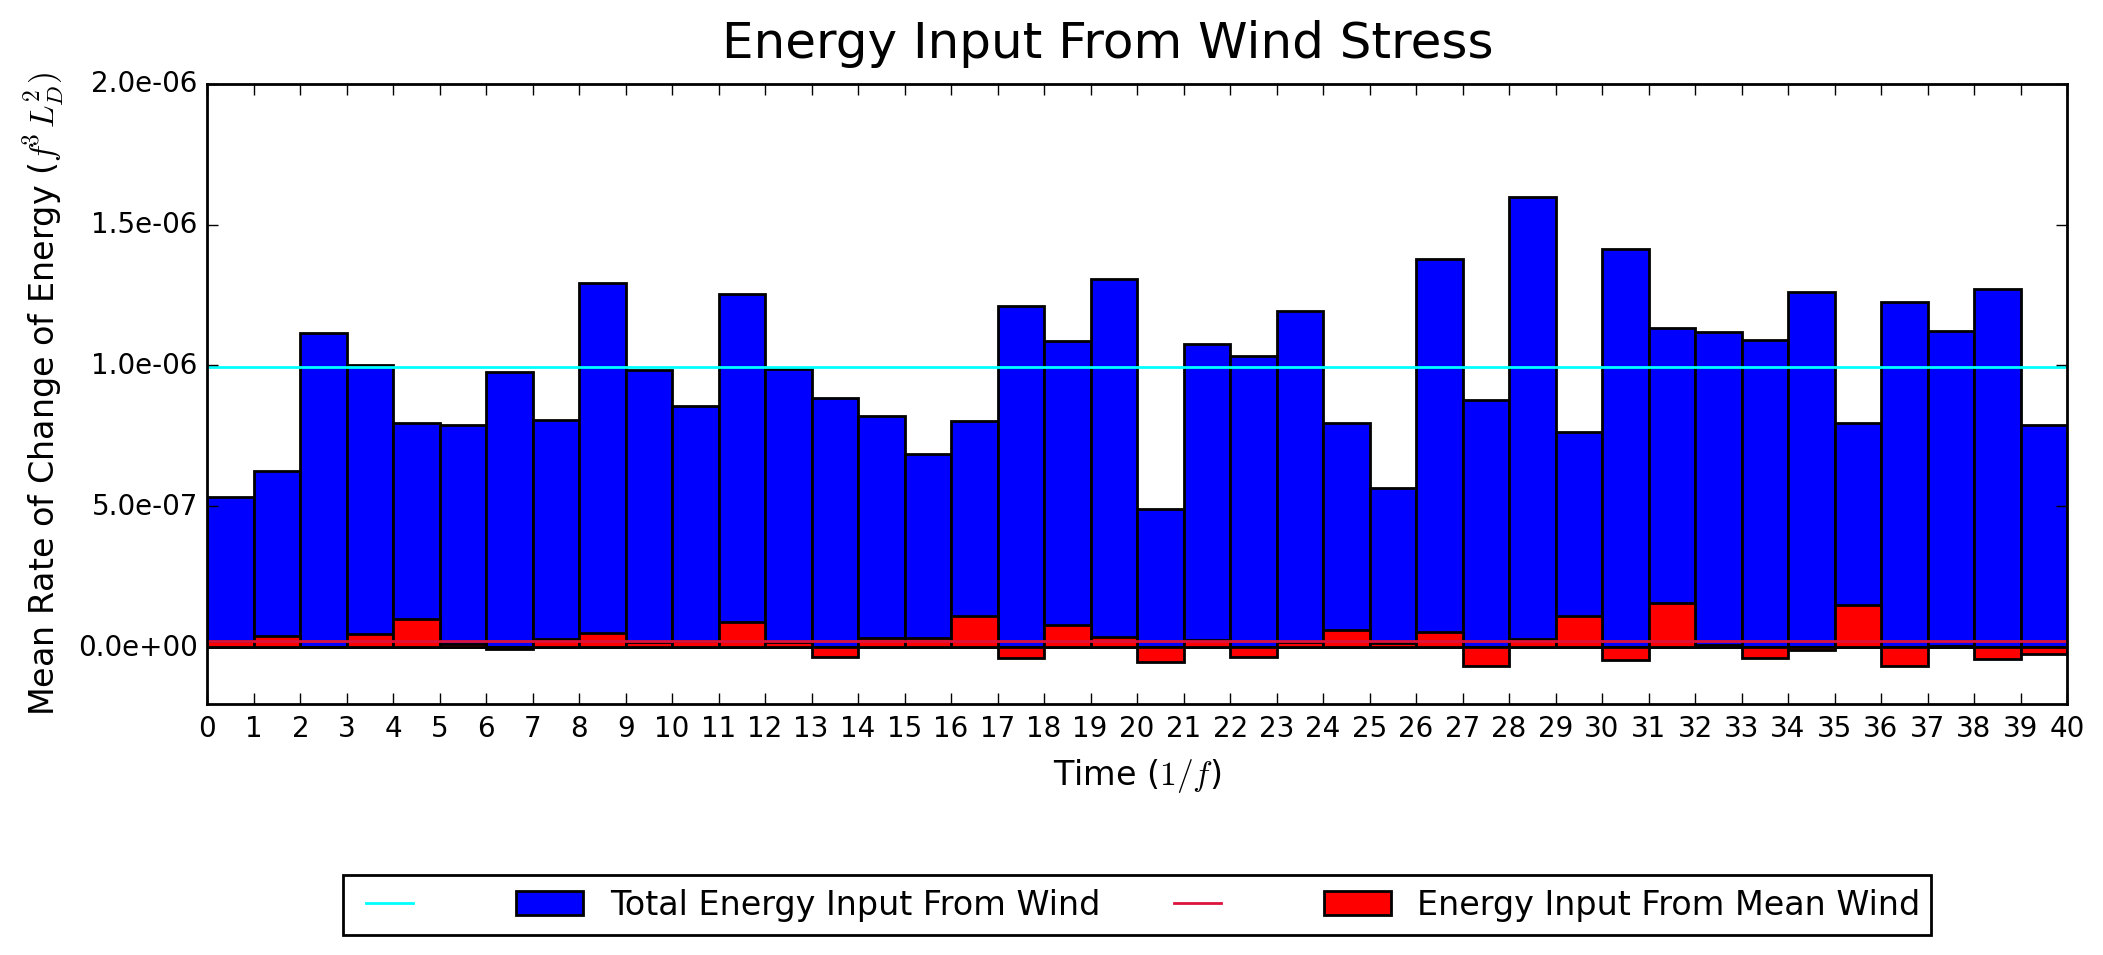
\includegraphics[width=\linewidth]{meaneddywind}
	\caption{ Energy input from the wind stress over each $10^{3}/f$ window. 
		The \textcolor{red}{red} bars show the energy input into the mean system,
		$\nthkmean{\boldsymbol{\tau}}\cdot\nthkmean{\boldsymbol{u}}$, in comparison
		to the total (mean + eddy) input (\textcolor{blue}{blue}), $\nthkmean{\boldsymbol{\tau}\cdot\boldsymbol{u}}
		=\nthkmean{\boldsymbol{\tau}}\cdot\nthkmean{\boldsymbol{u}}+\nthkmean{\nthkres{\boldsymbol{\tau}}\cdot\nthkres{\boldsymbol{u}}}$. The input into the mean system is around $2\%$ of
		the total input.}
	\label{fig:meaneddywind}
\end{figure}



\section{Momentum and Energy Conservation}

Exploiting the symmetry of the ridge, we can average in the zonal direction 
as well as in time. This allows us to decompose the flow into mean field 
varying only in the meridional direction and an eddy field. 

\hl{Model where the mean forcing is effectively zero. 
Hence the model is forced by a wind stress which is
absent from the mean system and hence forces the
system by 
invoking a turbulent cascade. Hence Eddy-Mean
interaction is entirely from the eddy to the mean.}

\section{\gls{pv} Conservation and Comparison of Mean \glspl{pv}}

\hl{An examination of the similarities and differences
of the two definitions of potential vorticity. 
A discussion of whether the thickness
weighted and tracer decomposition forms of the
PV eddy stresses can be used interchangeably.
This will be done by examining models with
different structures of potential vorticity.}


%\section{Strong Flow Models}

%more interesting situations, such as, models
%with a strong mean state, which hence
%generate there own eddy fields. E.g. Jets in
%channels or double gyres. Hopefully allowing 
%for the investigation of configurations where 
%Eddy Enstrophy is the constraining bound.


\chapter{Diagnostic Summary and Eddy-Mean Interaction Predictions}

Na\"{\i}ve attempt to parameterise eddies using the 
results from the previous chapters, depending
on what can be said about how the eddy stress can
be characterised and constrained by the topography,
eddy energy, eddy enstrophy etc. 

Likely will need to carry the time and spatial
evolution of eddy energy and eddy enstrophy and have
some sort of step function to turn on and off the
``GM like" and ``holloway like" parts of the parametrisation at appropriate moments.


\chapter{conclusions and discussions}

Summary of results.
Future work (keep this as unexplored possible ideas for now)

	 \printbibliography



\end{document}